\documentclass[12pt,a4paper,twoside]{book}
%\bfseries\scshape
%LINUX 
%\usepackage{isolatin1}
%WINDOWS
\usepackage[utf8]{inputenc}
\usepackage[spanish]{babel}
\selectlanguage{spanish}
\usepackage[sort&compress]{natbib}
\usepackage[T1]{fontenc} % fuente con codifiaci'on t1 para que el guinoado funcione bien
\usepackage{lmodern}
\usepackage{graphicx} % sirve para eps, ps y pdf (poner imagenes sin extension)
\usepackage{amsmath}
\usepackage{amssymb}
\usepackage{amsthm}
\usepackage{fancyhdr,fancybox}
\usepackage[nottoc]{tocbibind}
\usepackage[rigidchapters]{titlesec}
\usepackage{courier}

%\mtcselectlanguage{spanish}
%\setcounter{tocdepth}{1}
%\setcounter{parttocdepth}{1}

%\usepackage{times}
%\usepackage{helvet}

\decimalpoint % cambiar comas a puntos en los decimales
\usepackage[linktocpage]{hyperref}
\usepackage{breakurl} 
\usepackage{delarray}
%\usepackage{psfrag}
% \usepackage{subfigure}
\usepackage{subfig}
\usepackage{floatrow}
\usepackage{xspace}
\usepackage{float}
\usepackage{ifthen}
%\usepackage{moreverb}
%\usepackage{hyphenat}
%\usepackage{longtable}
\usepackage{pstricks,pst-plot,pst-node}
\usepackage{placeins}
\usepackage{booktabs}
\usepackage{indentfirst}
%\usepackage[spanish,ruled,vlined,figure]{algorithm2e}
% % % % % % % % % % % % % % % % % % % % % % % % % % % % % % % % % % % % 
\usepackage{url}
\usepackage{slashbox}
\usepackage{longtable}
\usepackage{multirow}
\usepackage{colortbl}
\usepackage{color}
\usepackage{lineno}
%\usepackage{tikz}
\usepackage{fancybox}
\usepackage{hyperref}
%\usepackage{bigfoot} %for split long footnotes
\usepackage{textcomp}
% 
% \usepackage{babel}
%box frame algorithm:
% \usepackage[charter]{mathdesign}
%\usepackage{eulervm}
\usepackage{enumitem}
\usepackage{xcolor}
%end box frame algorithm
%\usepackage{tabularx}
\usepackage{listings} %for c++ code
\definecolor{dkgreen}{rgb}{0,0.6,0}
\definecolor{gray}{rgb}{0.5,0.5,0.5}
\definecolor{mauve}{rgb}{0.58,0,0.82}

\lstset{ %
  language=C++,                % the language of the code
  basicstyle=\footnotesize,           % the size of the fonts that are used for the code
  %numbers=left,                   % where to put the line-numbers
  %numberstyle=\tiny\color{gray},  % the style that is used for the line-numbers
  %stepnumber=2,                   % the step between two line-numbers. If it's 1, each line  will be numbered
  %numbersep=5pt,                  % how far the line-numbers are from the code
  backgroundcolor=\color{white},      % choose the background color. You must add \usepackage{color}
  showspaces=false,               % show spaces adding particular underscores
  showstringspaces=false,         % underline spaces within strings
  showtabs=false,                 % show tabs within strings adding particular underscores
  frame=single,                   % adds a frame around the code
  rulecolor=\color{black},        % if not set, the frame-color may be changed on line-breaks within not-black text (e.g. commens (green here))
  tabsize=8,                      % sets default tabsize to 2 spaces
  captionpos=b,                   % sets the caption-position to bottom
  breaklines=false,                % sets automatic line breaking
  breakatwhitespace=true,        % sets if automatic breaks should only happen at whitespace
  title=\lstname,                   % show the filename of files included with \lstinputlisting;
  basicstyle=\scriptsize,                             % also try caption instead of title
  keywordstyle=\color{blue},          % keyword style
  commentstyle=\color{dkgreen},       % comment style
  stringstyle=\color{mauve},         % string literal style
  %escapeinside={\%*}{*)},            % if you want to add a comment within your code
  %morekeywords={*,...}               % if you want to add more keywords to the set
}
% 

% % % % % % % % % % % % % % % % % % % % % % % % % % % % % % % % % % % %
\usepackage{makeidx}

\newcommand{\titledframe}[2]{%
 \boxput*(0,1){\psframebox*{#1}}%
   {\psframebox[framesep=12pt]{\ttfamily #2}}}

\newcommand{\argmax}{\operatornamewithlimits{argmax}}

\newcommand{\mainidx}[1]{{\it #1}}
\newcommand{\boldidx}[1]{{\bf #1}}
\makeindex

\graphicspath{{figs/}}

%\hyphenation{gra-dien-te tra-ta-mien-to pers-pec-ti-va de-sa-rro-lla-do a-ce-le-r\'o-me-tros ca-rac-te-r\'is-ti-cas si-mi-la-res m\'e-to-dos co-rres-pon-den-cias des-cri-bi\'o glo-bal ca-rac-te-rís-ti-cos i-rre-le-van-tes i-ma-gen des-crip-tor gaus-sia-nos co-rres-pon-de-r\'an di-fe-ren-tes ni-vel si-guien-te res-pues-tas cons-tru-i-dos re-cha-za-da e-qui-va-len-tes co-li-nea-les su-pe-rar cap-tu-rado me-tros o-pe-ra-cio-nes rea-li-za-do o-pe-ra-ti-vos co-no-ci-mien-tos rea-li-dad rea-li-zar}

% PIE DE PAGINA para la primera pagina de cada capitulo
\fancypagestyle{plain} {
   \fancyhead[lrc]{}
	\renewcommand{\headrulewidth}{0pt}
   \fancyfoot[l]{}
   \fancyfoot[c]{}
   \fancyfoot[r]{\sf{\textbf{\thepage}}}
}

% ENCABEZADO para el resto de paginas
\pagestyle{fancy}
\fancyhf{}
\fancyhead[RO,LE]{\sf{\textbf{\thepage}}}
\fancyhead[LO]{\sf{\rightmark}}
\fancyhead[RE]{\sf{\leftmark}}
\setlength{\headheight}{15pt}
%\renewcommand{\chaptermark}[1]{\markboth{\chaptername \ \thechapter. #1}{}}
\renewcommand{\chaptermark}[1]{\markboth{#1}{}}
\renewcommand{\sectionmark}[1]{\markright{\thesection. #1}}

\def\fmfont{\fontsize\@xiipt{14.5}\selectfont\sffamily}

% FUENTES
%\renewcommand{\sfdefault}{phv}

% TITULOS DE CAPITULOS
\newcommand{\bigrule}{\titlerule[0.5mm]}


\titleformat{\chapter}[display]
{\sffamily\mdseries\Large}
{\filleft\MakeUppercase{\chaptertitlename} \Huge\bf\sf \thechapter}
{2ex}
{\titlerule
\vspace{4ex}%
\filright\Huge\sffamily\bfseries}
[\vspace{2ex}%
\bigrule]

% TITULOS de secciones y subsecciones
\titleformat{\section}[display]
{}{}{2ex}{\sffamily\bfseries\Large \thesection \ }[]

\titleformat{\subsection}[display]
{}{}{0ex}{\sffamily\bfseries \thesubsection \ }[]


% INDENTACION DE TODO EL DOCUMENTO: NULA
\parindent=0.2in
% SEPARACION DE PARRAFOS
\parskip=0.05in
\newtheorem{def_transf_proyectiva}{Definición}
%margenes para paginas impares mayores:
\let\tmp\oddsidemargin
\let\oddsidemargin\evensidemargin
\let\evensidemargin\tmp
\reversemarginpar
\selectlanguage{spanish}
\raggedbottom % para que no deje espacios gigantes entre secciones
\begin{document}

\thispagestyle{empty}
\sffamily\mdseries{
\begin{large}
\begin{center}
\mbox{
 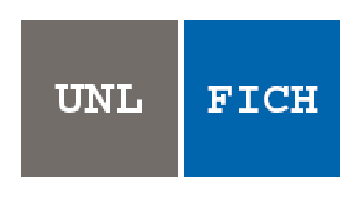
\includegraphics[scale=0.5]{fich_unl.eps}
}

  \textbf{Universidad Nacional del Litoral}\\
\vspace{0.5cm}
  \textbf{Facultad de Ingeniería y Ciencias Hídricas} \\
\textbf{Ingeniería en Informática} \\
\bigskip
Proyecto Final de Carrera
\end{center}
\end{large}

\vspace{1cm}

%\begin{center}
%  
\includegraphics[scale=0.3]{logounl}
%\end{center}

%\vspace{1cm}
\begin{LARGE}
\hspace{1cm}
\begin{center}
\textbf{Método para detección y seguimiento de objetos con aplicaciones en Realidad Aumentada}
\end{center}
\end{LARGE}


\vspace{2cm}
\hspace{3cm}
\begin{large}
\begin{tabular}{rl}
   Autor: & Pfarher, Christian Nicolás \\
   Director:& Dr. Albornoz, Enrique Marcelo \\
   Co-Director:& Dr. Martínez, Cesar 
\end{tabular}

\begin{center}
\vspace{2cm}
02 de Agosto de 2013
\end{center}
\end{large}
}

\rmfamily

\renewcommand{\thepage}{\roman{page}}

% \pagenumbering{roman}
% 
% 
%  \newpage
%  \thispagestyle{empty}
%  \mbox{}
%  \thispagestyle{empty}

\verb, ,\\
\vspace{8cm}

\begin{flushright}
\emph{Dedicado a... }
\end{flushright}


% 
% \newpage
% \thispagestyle{empty}
% \mbox{}
% 
% \newpage
% \thispagestyle{fancy}
% 
\chapter*{Agradecimientos}

Es para mi un verdadero placer utilizar este espacio para agradecer a aquellas personas que han estado a lo largo del desarrollo de este trabajo que ha marcado el fin de una etapa y el comienzo de otra.

Primeramente, debo agradecer de manera especial a mi familia y mi novia, por su incondicional apoyo ante las diversas situaciones que se han presentado a lo largo de este trabajo y de toda la carrera. Ellos han sido los pilares que me han facilitado de una u otra manera, cumplir el objetivo de graduarme como Ingeniero en Informática.

Quiero extender mi agradecimiento a mis directores de tesis por su apoyo, su confianza en mi trabajo y su capacidad para guiar mis ideas, que sin duda han realizado un gran aporte para la feliz concreción de este proyecto.

También, debo agradecer a mis amigos y compañeros de cursado que gracias a su disposición y ayuda han sido partícipes del largo camino que tuve que transitar para llegar a esta etapa final.

Por último, agradezco a aquellas personas que de una u otra forma, colaboraron o participaron en la realización de este trabajo.

\verb, ,




\vspace{1cm}
\emph{Mi más sincera gratitud,}

\begin{flushright}
Christian Nicolás Pfarher
Santa Fe, Argentina. \\ 02 de Agosto de 2013
\end{flushright}

%  \clearpage

\newpage
\thispagestyle{empty}
\mbox{}
\chapter*{Resumen}
\addcontentsline{toc}{chapter}{Resumen}
La detección de objetos es un área de estudio creciente y ha dado lugar a aplicaciones relevantes en diversas áreas (robótica \cite{conf/icra/2010}, vigilancia, \cite{5672610}, realidad aumentada \cite{5739718}, etc.), sin embargo aún queda mucho por explorar. En este trabajo, se presenta un método para la detección de objetos planos en cualquier perspectiva sin emplear marcadores, con procesamiento en tiempo real sobre flujo de video. Luego, se aplica en un prototipo de realidad aumentada.

El método desarrollado utiliza un detector y descriptor de características del estado del arte denominado SURF \cite{Bay:2008:SRF}. Para encontrar la posición del objeto se usa la homografía que se genera mediante la búsqueda de correspondencias de características entre una imagen patrón y el flujo de video, obtenido en tiempo real utilizando una cámara web de una computadora portátil. A los pasos generales propuestos en diferentes trabajos, aquí se le agregan etapas para mejorar la detección aumentando el rendimiento en cuanto a la velocidad y una serie de validaciones para evitar detecciones incorrectas y homografías que produzcan transformaciones defectuosas. También se proponen algunas técnicas sencillas para incrementar los detalles y mejorar la iluminación, a partir de experimentos y análisis de su comportamiento.

Finalmente se presentan dos prototipos: el primero localiza una imagen patrón en la escena, la cual puede presentarse escalada, rotada, y/o en perspectiva, y luego se sobrepone una fotografía en la región donde se detectó el patrón. El segundo prototipo fue desarrollado para una aplicación publicitaria, utilizando como imagen de patrón el packaging de un producto alimenticio y aplicando realidad aumentada para brindar información adicional del mismo.
%\clearpage

\newpage
\thispagestyle{empty}
\mbox{}
\chapter*{Prefacio}
\addcontentsline{toc}{chapter}{Prefacio}

El reconocimiento de objetos en imágenes ha sido y es un área de investigación que se ha mantenido en desarrollo y exploración constante. La habilidad de reconocer e identificar objetos en una imagen resulta esencial en áreas como vigilancia por video, imágenes médicas, realidad aumentada, etc.

El desarrollo de un motor propio de reconocimiento de objetos con aplicaciones en realidad aumentada, que sea fácilmente adaptable a aplicaciones específicas resulta de gran interés propio y para el grupo del SINC (Centro de Investigación en señales, sistemas e inteligencia computacional) \footnote{\url{http://fich.unl.edu.ar/sinc/}}. Si bien se puede encontrar software desarrollado, diferentes características de los mismos no lo hacen apropiado para su uso. Además, en el contexto local la realidad aumentada se ha convertido en un tema que constituye un ``nicho tecnológico y de mercado'' que resulta ampliamente atractivo para su desarrollo, investigación y explotación.

El término de realidad aumentada se usa para definir una visualización de un entorno físico del mundo real, cuyos elementos se combinan con elementos virtuales (imágenes, videos, sonidos, etc.), logrando crear una realidad mixta en tiempo real.

En este trabajo se presenta un método para la detección y seguimiento de objetos planos con aplicaciones en realidad aumentada, sin patrones artificiales y en un ambiente controlado. El método desarrollado es aplicado sobre flujo de video en tiempo real capturado con una cámara web estándar. El procedimiento tiene dos etapas principales: en una primera instancia se captura una imagen del objeto patrón, en una segunda etapa se captura flujo de video (imágenes objetivo) en tiempo real, para llevar a cabo la detección del objeto y el cálculo de su posición en la imagen, para luego ``enriquecer la realidad''.

Para llevar a cabo el procedimiento descripto anteriormente, se diseña un método que utiliza un detector rápido de características robustas denominado SURF \cite{Bay:2008:SRF}. El resultado de la detección y descripción de características es usado posteriormente en una etapa de búsqueda de coincidencias entre las características de la imagen patrón y la imagen objetivo. Tras encontrar los potenciales pares coincidentes, se procede a eliminar valores espurios y se calcula la homografía que resulta ser un mapeo perspectivo entre la imagen patrón y la imagen objetivo. Dado que es común que se obtengan falsos positivos al buscar la homografía, se propone un criterio para rechazar transformaciones erróneas provocadas por homografías mal estimadas. Todo este procedimiento es combinado con técnicas heurísticas para lograr un prototipo final optimizado para aplicaciones de realidad aumentada.
%  En este trabajo nos concentraremos en el reconocimiento y detección de objetos planos tales como imágenes, tapas de libros, logos etc. Este objeto plano será buscado en una secuencia de video capturada por una cámara web para su posterior localización mediante la utilización de búsqueda de homografía entre imágenes, valiéndose esta última des descriptores de características locales obtenidos mediante un método denominado SURF.

En lo que respecta a herramientas utilizadas para la codificación, existe variedad de software y bibliotecas para la manipulación de videos e imágenes. OpenCV (Open Source Computer Vision)\footnote[1]{\url{http://SourceForge.net/projects/opencvlibrary}} es una librería open source\footnote[2]{\url{http://opensource.org}} de visión computacional, escrita en C y C++, la cual puede ser ejecutada sobre diferentes sistemas operativos (Linux, Windows y Mac OS X). La misma, ha sido ampliamente adoptada como la herramienta de desarrollo en la comunidad de investigadores y desarrolladores en el campo de visión computacional \cite{citeulike:9456628}, debido a que fue diseñada para lograr gran eficiencia computacional, haciendo foco en el desarrollo de aplicaciones en tiempo real. Es por ello que, como base para la implementación del código fuente del método presentado, se utiliza la citada librería.

La tesis se encuentra organizada en cinco capítulos, como se explica a continuación.

En el Capítulo 1, se expone la motivación central del desarrollo de este proyecto, seguido de una reseña del estado del arte del reconocimiento de objetos y algunas de sus aplicaciones, haciendo hincapié en realidad aumentada. Posteriormente, se describen los objetivos generales y específicos, seguidos del los alcances del presente trabajo.

En el Capítulo 2, se tratan conceptos y métodos del marco teórico del procesamiento de imágenes, haciendo énfasis en la detección de características invariantes a escala y rotación. % mediante un algoritmo propuesto en la bibliografía.

El Capítulo 3 presenta el diseño del método propuesto basado en los fundamentos teóricos del capítulo anterior y utilizando el método de detección de características propuesto allí. También, se describen detalladamente las etapas del método propuesto, planteando mejoras y optimizaciones para las mismas con el fin de obtener un mejor desempeño en el tiempo de procesamiento, como así también, en la correcta detección del objeto en la escena.

En el Capítulo 4, se detallan los experimentos y los resultados obtenidos, donde se consideran variaciones de la iluminación y diferentes técnicas de realce de detalles sobre la imagen. Luego, se presentan dos experimentos y se propone un prototipo publicitario como resultado final del método desarrollado.

Finalmente, en el Capítulo 5, se exponen las conclusiones finales y los desarrollos futuros para corto, mediano y largo plazo.

\begin{flushright}
 Christian Nicolás Pfarher\\
 Santa Fe, Argentina. \\ 02 de Agosto de 2013
\end{flushright}

\clearpage

\tableofcontents

\listoffigures
% \renewcommand{\listtablename}{\'Indice de tablas}
% \renewcommand{\tablename}{Tabla}
% \listoftables
%\linenumbers
\newpage
\setcounter{page}{1}
\pagenumbering{arabic}
%\renewcommand{\thepage}{\arabic{page}}

%\dominitoc
   \section{Introducción}
\subsection*{Realidad aumentada}
\begin{frame}{Realidad aumentada}
\small{Un sistema de realidad aumentada (RA) reemplaza parte del mundo real con objetos virtuales, los cuales parecen coexistir en el mismo espacio que el ambiente real.}
\note[item]{$\rightarrow$ se crea una realidad mixta en tiempo real.}
  \begin{itemize}
    \item<1-> Introduce elementos virtuales en una escena captada de un entorno real.
    \item<2-> Trabaja interactivamente y en tiempo real.
    \item<3-> Detecta y realiza un ``seguimiento'' de objetos reales y virtuales entre sí.
    \item<4-> Realidad Aumentada no es Realidad Virtual.
    \item<5-> Según el grado de realismo o artificialidad:
    \begin{figure}[tbhp]
      \begin{centering}
	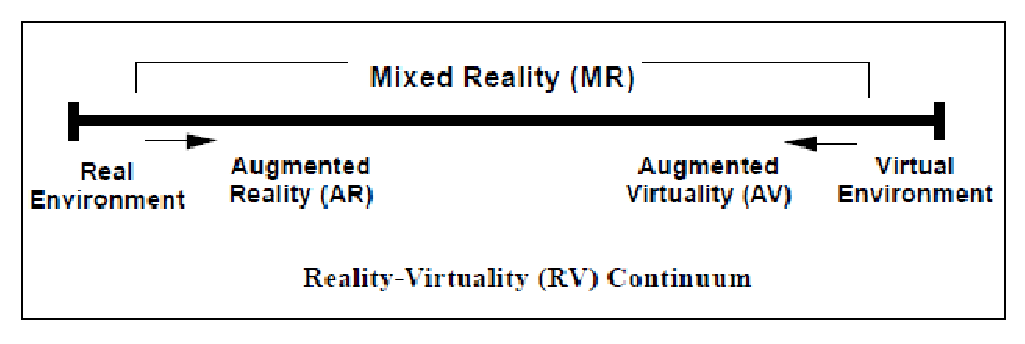
\includegraphics[width=6cm]{../../../img_ent1/reality_virtual.eps}
	\caption*{\tiny{Diagrama continuo de Realidad-Virtualidad. Milgram et al.}}
      \end{centering}
    \end{figure}
  \end{itemize}
\end{frame}

\begin{frame}{Sistemas y métodos para detección en RA}
    \begin{block}{Tipos de sistemas}
      \begin{itemize}
	    \item Basada en marcadores. \note[item]{es una imagen sintetica que altera el ambiente}
	    \item \textbf{No basada en marcadores} $\rightarrow$ características naturales de los objetos.
	      \note[item]{Marcelo: las características son de los objetos y NO DE LAS IMÁGENES}
      \end{itemize}
    \end{block}
   
     \begin{block}{Métodos para detección y seguimiento de objetos}
	\begin{itemize}
		\item Seguimiento basado en localización (GPS, acelerómetros, giroscopios, etc.)
		\item \textbf{Seguimiento óptico} $\rightarrow$ análisis e identificación de características a partir de la imagen.
		\item Una combinación de los dos anteriores.
	\end{itemize}
     \end{block}
\end{frame}

\begin{frame}{Aplicaciones - Ejemplos}
    \note[item]{Decir "marcadores" y  no patrónes!}
	\begin{center}{Aplicaciones - Ejemplos}
	  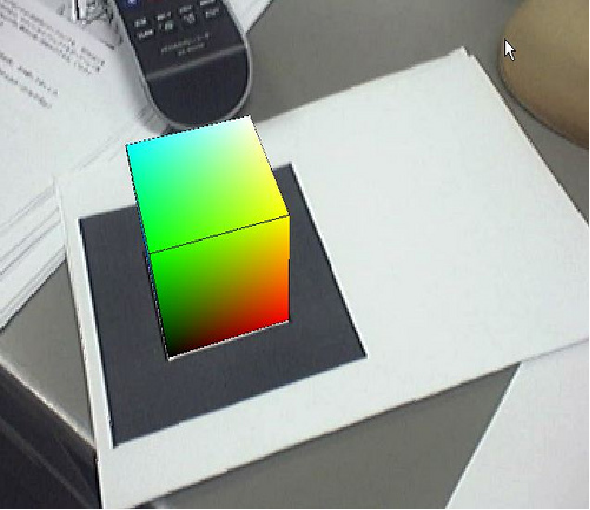
\includegraphics[width=7cm]{./img1/objeto_y_patron}
  	  
\includegraphics[width=7cm]{./img1/patrones}
	\end{center}
\end{frame}

\begin{frame}{Aplicaciones - Ejemplos}
      \note[item]{Decir "marcadores" y  no patrónes!}
	\begin{center}
	  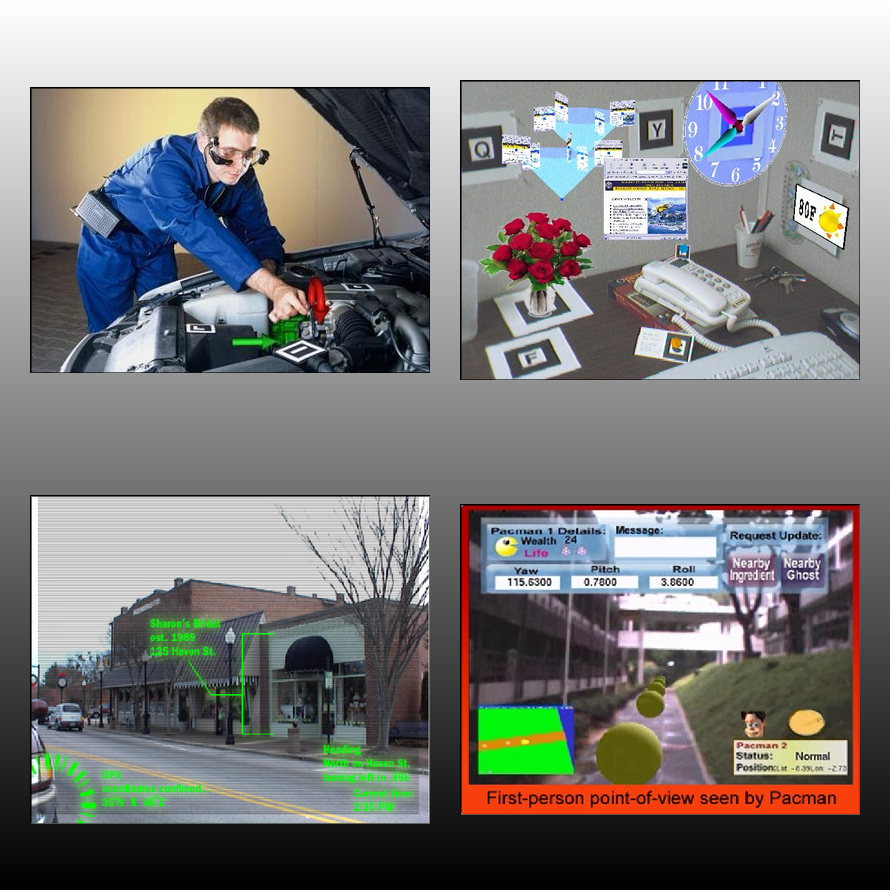
\includegraphics[width=7cm]{./img1/aplic1}
	\end{center}
\end{frame}
%%%%%%%%%%%%%%%%%%%%%%%%%%%%%%%%%%%%%%%%%%%%%%%%%%%%%%%%%
\subsection*{}
\begin{frame}{Motivación}
  \begin{itemize}
  \note[item]{Construir un método que permita reconocer objetos planos e identificar su posición en la imagen, en un ambiente controlado, para la posterior aplicación de realidad aumentada.}
  \item Desarrollo de un software propio de RA adaptable a aplicaciones específicas (comerciales, educativas, lúdicas, etc.)\footnote{SINC: Centro de Investigación en señales, sistemas e inteligencia computacional}
  \item No todas las aplicaciones trabajan en tiempo real.
  \item Muchos utilizan marcadores artificiales.
  \item Distribuidos bajo licencias privativas o costosos.
  \item Se trabaja con una tecnología que se encuentra en auge en estos tiempos.
      \note[item]{A cobrado gran imulso en el marketing, educación y e-commerce}
  \item El reconocimiento de objetos puede ser aplicado a diversidad de temáticas.
  \end{itemize}
\end{frame}

% \begin{frame}{Objetivos generales}
%   \begin{itemize}
%       \item Desarrollar un método para reconocer y seguir objetos en una secuencia de video digital y desarrollar un prototipo que haga uso del mismo aplicándolo a realidad aumentada.
%       \item Afianzar y extender los conocimientos adquiridos en el cursado de la carrera Ingeniería en Informática.
%   \end{itemize}
% \end{frame}
\subsection*{}
\begin{frame}
  \frametitle{Objetivos}
    \begin{itemize}
% 	\item Realizar el relevamiento del estado del arte en métodos utilizados para la detección y seguimiento de objetos en el Procesamiento Digital de imágenes.
	\item Diseñar y desarrollar un método reconocedor y seguidor de objetos planos en el flujo de video tomado por una cámara web estándar, sobre un ambiente controlado.
	\item Implementar el método en un algoritmo computacional que sea multiplataforma.
	%\item Optimizar el procesamiento llevado a cabo para lograr método desarrollado para que sea aplicable en tiempo real (\textbf{procesamiento}). 
	\item Optimizar el procesamiento para aplicarlo en tiempo real. 
	\item Implementar una aplicación prototipo específica (en el área de turismo, educación, publicidad, juegos u otros).
    \end{itemize}
\end{frame}

% \begin{frame}
% \frametitle{Alcances}
% \begin{itemize}
%   \item Se enmarcará en un sistema del tipo \textbf{sin marcadores} con método de reconocimiento del tipo \textbf{seguimiento óptico}.
%   \item El proyecto involucra el desarrollo de un prototipo para ser utilizado en una computadora con una cámara web estándar. Cabe aclarar, que no se pretende realizar una aplicación final específica y completa (estudio y diseño de interfaz amigable al usuario, introducción amigable de parámetros, etc.) orientada al uso de un usuario final.
%   \item Aunque no es un objetivo la implementación de varios métodos y su comparación, en una etapa previa se revisarán las características de algunos métodos para poder seleccionar alguno que se adecue a los requerimientos.
% \end{itemize}
% \end{frame}
%%
   %% \section {Operaciones morfológicas}
% algo
% \subsection{Conversión a Escala de grises}
% algo
% \subsection{Erosión}
% algo
% \subsection{Dilatación}
% algo
% \subsection{Bounding Box}
% algo
% \subsection{Convex Hull}
% algo
%%%%%%%%%%%%%%%%%%%%%%%%%%%%%%%%%%%%%%%%%%%%%%%%%%%%%%%%%%%%%%%%%%%%%%%%%%%%%%%%%%%%%%%%


%%%%%%%%%%%%%%%%%%%%%%%%%%%%%%%%%%%%%%%%%%%%%%%%%%%%%%%%%%%%%%%%%%%%%%%%%%%%%%%%%%%%%%%%
 %problema y generalidades
   %\chapter{Fundamentos Teóricos}
\label{c:fundamentosteoricos}

\vspace{1cm}

En este capítulo se presentan los principales fundamentos teóricos para llevar a cabo el presente trabajo.

Primeramente se describen las operaciones morfológicas: conversión a escala grises sobre una imagen, erosión, dilatación, bounding box y convex hull.

Luego, se presentan los conceptos más importantes de las características locales junto con sus propiedades más significantes como así también una distinción de los los detectores dependiendo del uso de los mismos. Además, se hace una breve síntesis de las características locales junto a sus propiedades más importantes con una discusión sobre las mismas.

Finalmente, se detalla los fundamentos de un método de detección características, haciendo incapie en método SURF y su relación con SIFT. Además, se describe la correspondencia de características entre imágenes mediante  la búsqueda del vecino más cercano ayudado del método estadístico RANSAC para la eliminación de correspondencias espurias.

% http://opencv.willowgarage.com/documentation/cpp/geometric_image_transformations.html
\newpage

\subsection{otra cosa}
      En este trabajo, nos enfocaremos en un detector y descriptor invariante a escala y en el plano. Tanto el detector como el descriptor no utilizarán información de color, sino que se valdrán de una imagen en escala de grises para llevar a cabo el procedimiento. Estos, parecen ofrecer un buen compromiso entre la complejidad de las características y la robustez a las deformaciones que comúnmente ocurren. La distorsión o torcimiento, escalado no isótropo\footnote{En geometría euclídea, el \textbf{Escalado uniforme} o \textbf{Escalado isótropo} es una transformación lineal que incrementa o decrementa un objeto por un factor de escala el cual es el mismo en todas las direcciones. El resultado del escalado, es similar (en sentido geométrico) al original. Si se utiliza al menos un factor de escala diferente para un eje de coordenadas, se está en presencia de un \textbf{Escalado no uniforme} o \textbf{Escalado no isótropo} resultando en un cambio en la forma del objeto.} y efectos de la perspectiva se asumen que son alteraciones de segundo orden que son cubiertos en cierto grado por la robustez general del descriptor seleccionado.

      Un detector de puntos de interés usado recientemente es el Detector rápido de características robustas o SURF (Speeded Up Robust Features) \cite{citeulike:9456628, citeulike:7676197, Bay:2008:SRF, bb53077, TuytelaarsM07, Bay:2008:SRF, BouGar}. El método SURF es un detector y descriptor invariante a escala y rotación (logrado mediante la asignación de una orientación a cada punto clave detectado) que posee buenas propiedades de repetibilidad, distintividad y robustez permitiendo además calcularse y ser comparado rápidamente respecto a otros métodos. El mismo está basado en conceptos del algoritmo de Transformación de características invariante a la escala o SIFT (Scale Invariant Feature Transform) \cite{citeulike:3484001, citeulike:9456628, citeulike:7676197, bb53077, journals/tvcg/WagnerRMDS10, TuytelaarsM07, bb48614, Nixon:2002:FEI, BouGar, 5739718, conf/ismar/2004}. 
      -------------
      Como se mencionó anteriormente, el algoritmo SURF define la localización y escala para cada una de las características detectadas. Este factor de escala, puede ser usado para definir el tamaño de una ventana alrededor de cada punto característico, de tal manera de poder definir un área vecina que incluya la misma información visual, sin importar la escala en que el objeto fue fotografiado. Así, esta información visual incluida en esa vecindad, resulta útil para caracterizar el punto clave y ayuda en la distinción del mismo de otros similares.

      Para describir el área vecina de los puntos característicos, se usan descriptores de características, que usualmente (en el caso de comparación entre imágenes) son vectores N-dimensionales que resultan ser invariantes a cambios de iluminación y a pequeñas deformaciones de perspectivas (en el caso ideal). Además, resultan potencialmente usables para ser comparados mediante el uso de una métrica de distancia, como por ejemplo: la distancia euclídea. 

      En el caso del algoritmo SURF, el descriptor por defecto posee 64 elementos (SIFT utiliza 128) y este vector caracteriza el patrón de intensidad en el área que rodea a un punto característico. Cuanto más similares sean dos puntos característicos, más cercanos serán sus vectores descriptores. 

      Así, dadas dos imágenes de la misma escena, primeramente se extraen los puntos claves y los descriptores asociados con cada uno de ellos para ambas imágenes. Luego, cada vector descriptor en la primer imágen es comparado con todas los vectores descriptores de la segunda imágen. El par que obtiene la menor distancia entre ellos, es considerado la mejor coincidencia para dicha característica. Luego el proceso es repetido para todas las características de la primer imágen. Este esquema básico para coincidencias es conocido como coincidencias por fuerza bruta. El método termina considerando los 25 más cercanos y los demás pares son descartados.

\section{Pasos para implementación del algoritmo SURF}
\begin{itemize}
 \item Se toma una imagen del objeto a detectar y se detectan los puntos claves junto con sus descriptores asociados. Es importante que esta imagen contenga solo el objeto a detectar. Dicha detección se realizan mediante SURF cuyos pasos pueden resumirse:%\footnote{\url{http://robocv.blogspot.com.ar/2012/02/real-time-object-detection-in-opencv.html}}:
  \begin{enumerate}
    \item Busca puntos interesantes en la imagen usando matrices hessianas.
    \item Determina una orientación para cada punto encontrado.
    \item Usa wavelets haar en una región cuadrada orientada alrededor del punto clave para buscar los gradientes de intensidad en la dirección $x$ e $y$. Esta región cuadrada es dividida en 16 sub regiones, y cada sub región construye 4 características (que son básicamente sumas de cambios de gradientes), resultando el descriptor surf en un vector de 64 dimensiones.
  \end{enumerate}
 \item Se repite el paso anterior para cada fotograma capturado por la cámara.
 \item Se emplea la la estrategia de correspondencias para buscar las coincidencias validas.
 \item Para obtener un bounding box alrededor del objeto detectado, las coincidencias validas, se busca la homografía que transforma los puntos de la imagen de entrenamiento a la imagen objetivo. Usando esta homografía, se transforman las 4 esquinas de la imagen de entrenamiento y se coincideran estos 4 puntos como vertices y dibujar una caja en el frame de video. Se dibuja la caja solo si se encuentran 4 o más buenos macheos.
\end{itemize}

\section{Filtrado de imágenes}
El filtrado es una de las principales tareas en el procesamiento de imágenes y de señales. Es un proceso que busca extraer ciertos aspectos de la imágen que resultan ser información conveniente o importante en el contexto de una aplicación dada. El filtrado, remueve ruido, extrae características visuales interesantes, permite el escalado de imágenes, etc.

Caundo miramos una imagen, se pueden observar como los niveles de grises o colores están distribuidos en la misma. Las imágenes defierien unas de otras porque tiene diferentes distribución de niveles de grises. Existe otro punto de vista desde el que una imágen puede ser analizada. Se puede mirar la variación de niveles de grises que estan presentes en una imágen. Algunas imagenes contienen grandes areas de intensidad casi constante (por ejemplo una imágen de un cielo despejado) mientras que en eotras imagenes, las intensidaddes de grises varian rapidamente sobre la imagen (una escena colmada de objetos pequeños). Por lo tanto, observando la frecuencia de estas variaciones en uan imagen constituyen otra forma de caracterizar una imagne. Este punto de vista es referido como dominio de la frecuencia, mientras que la caracterízación de la imágen mediante la observación de la distribución de niveles de grises es referida como dominio espacial.

El análisis en el dominio de las frecuencias descompone una imagen segun su contenido frecuencial en altas y bajas frecuencias. Las frecuencias bajas, se corresponden con areas donde las intensidades varian lentamente, mientras que las altas son generadas por cambios de intensidades bruscos o apruptos. 

Bajo el dominio de las frecuencias, un filtro es una operación que amplifica ciertas bandas de frecuencias de una imágen mientras disminuye o bloquea otras. Así un filtro pasa bajos, es un filtro que elimina las compoennetes de altas frecucncias de una imágen y reciprocamente un pasa altos elimina las componenetes de bajas frecuencias.

Filtrar una imágen con un filtro pasa bajos, reduce la amplitud de la variación en la imágen (se reemplaza cada pixel por un promedio de pixles alrededor) produciendo el borroneado de la imágen. Esta operación se lleva a cabo mediante una máscara o kernel la cual es desplazada sobre cada pixel de la imágen mutiplicandose cada pixel correspondiente por el peso asociado en esta máscara. Esta operación es conocida como convolución.



% \paragraph{Puntos de interés basados en la Matriz Hessiana}


% La detección de objetos usando SURF resulta invariante a escala y rotación y no requiere de un largo y tedioso entrenamiento como en el caso de detectores basados en un clasificador de Haar en cascada. Debido a que este método es invariante a rotación, es posible detectar objetos en cualquier orientación a diferencia de otros detectores como los que utilizan características Haar.

% 
% \subsection{Descripción de las características}
% La descripción de las características es un proceso de crear un vector de números que de alguna manera describan a una característica local (feature descriptor). Este puede ser usado para la correspondencia de características entre imágenes. Idealmente, los descriptores deberían ser invariantes a escala, traslación, rotación y a varios cambios en la escena, como luminosidad, ruido o borroneado, de forma que la característica local pueda ser identificada en diferentes imágenes con condiciones variantes (idealmente).
% 
% Existen varios algoritmos para descripción de características, pero aquí se trabajará con el que propone el método SURF.
% 
% Usaremos la descripción de características para construir una base de datos de puntos claves o keypoints conocidos de un objeto plano (imagen de entrenamiento) y luego buscaremos este en la imagen objetivo (fotograma del flujo de video) mediante la comparación de ambos descriptores. Tanto el método SIFT como el SURF operan con la función Gaussiana $G$, el Laplaciano del Gausiano $L$ (su derivada de segundo orden) y la imagen convolucionada $C$. Estos han sido definidos en la ecuación \ref{eq:gaussian_function}, \ref{eq:result_convolution_image}, \ref{eq:laplacian_of_gaussian_function} donde $x,y$ son las coordenadas expresadas en píxeles y $sigma$ representa la escala mencionada en párrafos anteriores.
% \begin{equation}
%  \label{eq:gaussian_function}
%  G_{\sigma}(x,y)=\frac{1}{\sqrt[]{2\pi\sigma^{2}}}e^{\frac{-(x^{2}+y^{2})}{2\sigma^{2}}}
% \end{equation}
% \begin{equation}
%  \label{eq:result_convolution_image}
%  C_{\sigma}(x,y)=G_{\sigma}(x,y)*I(x,y)
% \end{equation}
% \begin{equation}
%  \label{eq:laplacian_of_gaussian_function}
%  L_{\sigma}(x,y)=\Delta G_{\sigma}(x,y)=\frac{\partial\text{\texttwosuperior}}{\partial x\text{\texttwosuperior}}G_{\sigma}(x,y)+\frac{\partial\text{\texttwosuperior}}{\partial y\text{\texttwosuperior}}G_{\sigma}(x,y)
% \end{equation}
% %end: extraido de parte 3
% % 
% % 
% % 
% % El primer paso, para construir el descriptor, consiste en fijar una orientación reproducible basada en la información de una región circular alrededor del punto de interés. Luego, se construye una región cuadrada alineada con la orientación seleccionada, y se extrae el descriptor SURF de ella.
% % % 
% % % \subsubsection{Asignación de la orientación}
% % % \label{asignacion_orientacion_susbsection}
% % % Con el objetivo de lograr invariancia a la rotación, se identifica una orientación que sea reproducible para los puntos de interés. Para este propósito, primeramente se calculan las respuestas de la Wavelet Harr en la dirección ``x'' y ``y'' con los kernels de la Fig. \ref{fig:simplekernels} en una vecindad circular de radio $6\sigma$ alrededor del punto de interés (donde $\sigma$ representa la escala a la que fue detectado el punto de interés).
% % % 
% % % Una vez que han sido calculadas las respuestas wavelets y ponderadas por una Gaussiana centrada en el punto de interés (con un valor de $2.5\sigma$) estas son representadas mediante un vector en el espacio, con las respuestas de intensidad horizontales a lo largo de la abscisa y las verticales a lo largo de la ordenada. 
% % % 
% % % La orientación dominante es calculada como la suma de todas las respuestas dentro de una ventana deslizante con un ángulo de ($\pi/3$) parámetro seleccionado experimentalmente según lo define el autor. El mayor vector entre ellos es el que define la orientación dominante del punto de interés.
% % % 
% % % \subsubsection{Componentes del descriptor}
% % % Para la extracción del descriptor, el primer paso consiste en construir una región cuadrada centrada alrededor del punto de interés y orientada en la dirección de la orientación calculada en la subsección \ref{asignacion_orientacion_susbsection}. El tamaño de la ventana es $20\sigma$.
% % % 
% % % La región cuadrada luego es dividida regularmente en subregiones cuadradas más pequeñas de 4x4. Denominando $dx$ a la respuesta de la wavelet Harr en la dirección horizontal Fig. \ref{fig:simplekernels1} y $dy$ la respuesta en la dirección vertical Fig. \ref{fig:simplekernels2} donde ``Horizontal'' y ``Vertical'' aquí, son definidas en relación a la orientación seleccionada del punto, se calcula para cada subregión las respuestas del kernel $dx$ y $dy$ en un área localizada y regularmente espaciada cada 5x5 puntos(el tamaño del kernel es $2\sigma$). Hay que aclarar que con el objetivo de dar mas importancia a los píxeles vecinos mas cercanos al punto clave, las respuestas del kernel se ponderan con un Gaussiano centrado en el punto de interés (con $\sigma=3.3$) incrementando la robustez frente a deformaciones geométricas y errores de localización.
% % % 
% % % % \begin{figure}[tbhp]
% % % %    \centering
% % % %    %%----primera subfigura----
% % % %    \subfloat[]{
% % % %         \label{fig:simplekernels1}         %% Etiqueta para la primera subfigura
% % % %         \includegraphics[scale=0.35]{../img_ent2/simplekernels1har}}
% % % %    \hspace{0.1\linewidth}
% % % %    %%----segunda subfigura----
% % % %    \subfloat[]{
% % % %         \label{fig:simplekernels2}         %% Etiqueta para la segunda subfigura
% % % %         \includegraphics[scale=0.35]{../img_ent2/simplekernels2har}}
% % % %     \caption[Kernels aplicados para el cálculo de la respuestas Haar]{Kernels aplicados en la vecindad de un punto característico.}
% % % %    \label{fig:simplekernels}                %% Etiqueta para la figura entera
% % % % \end{figure}
% % % 
% % % Las respuestas wavelet $dx$ y $dy$ son sumadas sobre cada subregión y forman un primer conjunto de entradas para el vector de características. Con el propósito de dar información acerca de la polaridad de los cambios de intensidad, también se extrae la suma de los valores absolutos de las respuestas: $\left|dx\right|$ y $\left|dy\right|$. Así, cada subregión tiene un vector descriptor de cuatro dimensiones cuya expresión es: 
% % % % \begin{equation}
% % % % \left[\sum dx\qquad\sum dy\qquad\sum \left|dx\right|\qquad\sum \left|dy\right|\right]
% % % % \label{equation_suma} 
% % % % \end{equation} 
% % % Esto, resulta en un vector descriptor para todas las subregiones de $4x4$ de un tamaño de 64 elementos $(4x4x4)$. Se debe tener en cuenta que las respuestas de las wavelets son invariantes a un sesgo en la iluminación y que la invariancia de contraste (un factor de escala) se consigue transformando el vector en uno unidad.
% % % 
% % % La Fig. \ref{fig:respuesta_descriptor}, muestra en una subregión las propiedades del descriptor para tres imágenes distintas que poseen diferentes patrones de intensidad. Una combinación de dichos patrones locales de intensidad, daría como resultado un descriptor posible de distinguir.
% % % 
% % % \begin{figure}[tbhp]
% % %    \centering
% % %         \includegraphics[scale=0.4]{../img_ent2/egharrresponses}
% % %     \caption[Respuestas del descriptor SURF]{Las entradas del descriptor de una subregión, representan la naturaleza del patrón de intensidad subyacente. Izquierda: en el caso de una región homogénea, todos los valores son relativamente bajos. Centro: En presencia de frecuencias en la dirección ``x'', el valor $\sum \left|dx\right|$ es alto, mientras los demás son bajos. Derecha: Si la intensidad se incrementa gradualmente en la dirección ``x'', ambos valores: $\sum dx$ y $\sum \left|dx\right|$ son altos.}
% % %    \label{fig:respuesta_descriptor}                %% Etiqueta para la figura entera
% % % \end{figure}
% % % 
% % % De esta forma, buscar correspondencias con invariancia a escala entre imágenes es alcanzable mediante las características y descriptores que se obtiene con SURF.
% % % 
% % % \bigskip
% % % \bigskip
% % % \bigskip

% \fbox{\footnotesize \parbox[c]{.9\columnwidth}{\textbf{\underline{\emph{Diferencias generales respecto del algoritmo SIFT:}}} 
% SIFT es un detector y descriptor de características en el que se propone la detección de características invariante a la escala mediante la búsqueda en imágenes a múltiples escalas. El método, resulta invariante a traslación, rotación y parcialmente a cambios en la iluminación.
% 
% Las características son identificadas como extremos espacio-escala de la función diferencia de gaussianos (DoG). Esta función es aplicada a una pirámide de imágenes creada desde la imagen original mediante el continuo difuminado y desescalado (sub-muestreo). 

% La función DoG $D$ es una aproximación al Laplaciano del Gaussiano donde $k$ es el factor de escala entre las escalas vecinas \ref{eq:dog_aprox_laplacian}.
% 
%  \begin{multline}
% \label{eq:dog_aprox_laplacian}
% D_{\sigma}(x,y)=\left[G_{k\sigma}(x,y)-G_{\sigma}(x,y)\right]*I(x,y)\\
% =C_{k\sigma}(x,y)-C_{\sigma}(x,y)
% \end{multline} 
% 
% Un punto es seleccionado como extremo local cuando se cumple la condición de que los nueve vecinos en la escala superior e inferior y los ocho vecinos son todos mayores o todos menores que el punto seleccionado (eliminación de los no máximos\footnote{\url{http://users.ecs.soton.ac.uk/msn/book/new_demo/nonmax/}} locales del $\det(\mathcal{H}_{approx})$ en una vecindad de $3x3x3$ del punto). Un esquema gráfico puede ser observado en la Fig. \ref{fig:selected_scale_point}. La posición de los puntos claves es además interpolada a la posición sub-pixel usando la expansión de taylor de la función DoG. Luego de esto, los puntos inapropiados, tales como los de bajo contraste o bordes son rechazados.
% 
% Una vez que los puntos son localizados o adquiridos usando un detector de características, se calcula el descriptor para el punto. El mismo esta basado en la orientación del gradiente de la vecindad del punto clave. Este proceso es ilustrado en la figura \ref{fig:selected_scale_point} derecha. Las orientaciones son recogidas en una vecindad alrededor del punto clave. La figura muestra un área vecina de $2x2$, pero existen implementaciones con tamaños de $4x4$. Así, ocho orientaciones son obtenidas por cada contenedor, por lo que resulta en un vector de $4x4x8=128$ elementos, el cual es llamado descriptor SIFT del punto clave. %El algoritmo SIFT es el estándar defacto para la descripción de características.
% 
% El algoritmo SIFT, también define su propio descriptor. Se basa en la magnitud del gradiente y orientación calculado en la escala del punto clave considerado. Como en el caso de los descriptores SURF, el área vecina escalada del punto clave es dividido en 4x4 sub-regiones. Para cada una de estas regiones, se construye un histograma de 8 clases de las orientaciones del gradiente (ponderados por su magnitud y por una ventana gaussiana global centrada en el punto clave). Luego, el vector descriptor es construido de las entradas de este histograma. Hay 4x4 regiones y 8 clases por histograma, lo que nos da un descriptor de una longitud de $4x4x8=128$ elementos. 
% 
% La diferencia más marcada los descriptores SIFT y SURF, es principalmente la velocidad y precisión. Los descriptores SURF están mayormente basados en diferencias de intensidades y se valen de las imágenes integrales y filtros caja para obtener las respuestas para varias escalas de siendo más rápidos y eficientes de calcular; por otro lado, los descriptores SIFT son considerados generalmente más precisos en buscar la característica correcta (coincidencia más exacta), pero llevando más tiempo de cálculo. Otra de las diferencias fundamentales, es que en SIFT la dimensión escala es creada mediante el desescalado de la imagen, mientras que en SURF se incrementa el tamaño del filtro manteniéndose constante el tamaño de la imagen.
% }}

%%%%%%%%%%%%%%%%%%%%%%%%%%%%%%%%%%%%%%%%%%%%%%%%%%%%%%%%%%%%%%%%%%%%%%%%%%%%%%%%%%%%%%%%%%%%%%%%%%%%%%%%%
%%%%%%%%%%%%%%%%%%%%%%%%%%%%%%%%%%%%%%%%%%%%%%%%%%%%%%%%%%%%%%%%%%%%%%%%%%%%%%%%%%%%%%%%%%%%%%%%%%%%%%%%%
%  Local Feature View Clustering for 3D Object Recognition - paper David LOWE
% Cada característica SIFT es representada por un vector con medidas locales de la imagen, de tal manera de ser invariante a la traslación, escalado y rotación y parcialmente invariante a cambios de iluminación y deformaciones locales. Una imagen típica producirá gran cantidad de características que se sobre solapen en un rango de varias escalas  que formaran una representación redundante de la imagen original. La naturaleza local y multi escala de la características la hará insensitiva al ruido, desorden y oclusiones, mientras que las propiedades de los detalles locales de la imagen representados por las características la harán altamente selectivas para realizar un match con grandes bases de datos de características previamente almacenadas.
% 
% La localización de las características SIFT son eficientemente detectadas identificando el máximo y mínimo de una función diferencia de gaussianos en el espacio escala. En cada localización, una orientación es seleccionada como el pico del histograma del gradiente de las orientaciones de la imagen local. Un vector de características es así construido mediante la medida de gradientes locales en la imagen en una región alrededor de cada punto localizando en coordenadas relativas a la localización, escala y orientación de la característica. La localización del gradiente son borroneadas para reducir la sensibilidad a pequeñas deformaciones locales de la imagen, como ser un cambio del punto de vista. Resumiendo, el enfoque de SIFT transforma las características locales de la imagen en relación con marcos de coordenadas que se espera que sean estables a través de múltiples puntos de vista de un objeto.

% El tamaño de la región de la imagen que es muestreada por cada característica es variable, pero los experimentos de este paper usan vectores de 128 elementos por cada característica para muestrear ocho orientaciones de gradientes sobre una región de 4x4. El uso de 128 elementos (un vector largo) es útil para dar un grado mayor de selectividad al hacer un maching de características con una base de datos, resultando en mejore precisión y eficiencia.
%%%%%%%%%%%%%%%%%%%%%%%%%%%%%%%%%%%%%%%%%%%%%%%%%%%%%%%%%%%%%%%%%%%%%%%%%%%%%%%%%%%%%%%%%%%%%%%%%%%%%%%%%
%%%%%%%%%%%%%%%%%%%%%%%%%%%%%%%%%%%%%%%%%%%%%%%%%%%%%%%%%%%%%%%%%%%%%%%%%%%%%%%%%%%%%%%%%%%%%%%%%%%%%%%%%
%%%%%%%%%%%%%%%%%%%%%%5
%%%%%%%%%%%%%%%%%%%%%%
%%%%%%%%%%%%%%%%%%%%%%%%5
%%%%%%%%%%%%%%%%%%%%%%%%%%%%%

%%%%%%%%%%%%%%%%%%%%%%%%%%%%%%%%%%%5
%%%%%%%%%%%%%%%%%%%%%%%%%%%%%%%%%%%%%%5%
%%%%%%%%%%%%%%%%%%%%%%%%%%%%%%%%%%%%%5
%%%%%%%%%%%%%%%%%%%%%%%%%%%%%%%%%

% no me gusto como esta definido esto:
% \section{SURF: Speeded-Up Robust Feature}
% %http://www.ipol.im/pub/algo/or_speeded_up_robust_features/#lowe2004
% SURF es un algoritmo que sirve para la representación y comparación local de imágenes. Similarmente a SIFT \cite{Lowe2004}, este método selecciona los puntos característicos más destacadas de una imagen en una representación de espacio-escala lineal y construye características locales basados en la distribución del gradiente de la imagen. Una de las principales características de SURF sobre SIFT, radica en que calcula más rápidamente los operadores diferenciales aproximados en el espacio-escala, basado en la Representación de Imágenes Integrales y en los filtros tipo caja o Box \cite{conf/nips/SimardBHL98} lo cual permite realizar aplicaciones en tiempo real aplicadas al seguimiento y reconocimiento de objetos.
% 
% \subsection{Esquema del algoritmo}
% El algoritmo SURF esta compuesto de tres pasos consecutivos:
% \begin{enumerate}
%  \item detección de puntos de interés
%  \item descripción de los puntos de interés
%  \item correspondencias de las características.
% \end{enumerate}
% 
% Los primeros dos pasos (al igual que con el método SIFT), recaen sobre la representación espacio-escala \cite{Lindeberg94scale-spacetheory} y los operadores diferenciales de primer y segundo orden.
% % La originalidad del método SURF, es que se ha incrementado la velocidad de cálculo con estos operadores a través del uso de imágenes integrales y filtros tipo caja (box filters).
% 
% En el paso de detección, los máximos locales del operador determinante Hessiano aplicado al espacio-escala es calculado para seleccionar los puntos candidatos destacados. Estos, luego son validados si la respuesta esta por encima de un valor de umbral determinado. Luego tanto la escala como la localización de estos candidatos son refinados usando un procedimiento iterativo para adaptarse a una función cuadrática.
% 
% El propósito del segundo paso es construir un descriptor que sea invariante a cambios de punto de vista sobre un vecindario local del punto de interés detectado. Recordemos que la localización de este punto en el espacio-escala provee invarianza a cambios de escala y traslación. Para obtener invarianza a rotación, una orientación dominante es definida mediante la distribución de la orientación del gradiente local estimado mediante las wavelets Haar. Haciendo uso de la grilla de localización espacial, se construye un descriptor de 64 dimensiones, correspondiente al histograma local de las respuestas de las wavelets Haar.
% 
% El tercer paso compara los descriptores de dos imágenes para encontrar coincidencias. La comparación exhaustiva es calculada mediante la distancia euclídea entre todos los potenciales pares y mediante el uso de una relación de distancia para reducir las falsas correspondencias. Además esto se combina con una técnica basada en un algoritmo denominado RANSAC para corroborar la consistencia geométrica (geometría epipolar). Luego de que estos filtros eliminan todas las coincidencias sospechosamente falsas, uno puede estar más seguro que las coincidencias restantes son reales y corresponden a la misma escena vista desde diferentes puntos de vistas.
% 
% \subsection{Algoritmo paso por paso}
% \begin{enumerate}
%  \item Calculo de la imagen integral de la imagen de entrada.
%  \item Detección de puntos de interés:
%   \begin{itemize}
%    \item Cálculo del operador Hessiano discreto a diferentes escalas usando Filtros caja.
%    \item Selección de las respuestas máximas del determinante de la matriz hessiana en el espacio escala (umbral)
%    \item Refinamiento de la localización de los puntos de interés mediante interpolación cuadrática
%    \item Guardado de los puntos de interés con el signo del Laplaciano.
%   \end{itemize}
%  \item Construcción del descriptor local:
%   \begin{itemize}
%    \item Estimación de la orientación dominante de cada punto de interés.
%    \item Cálculo del descriptor (vector de 16x4) correspondiente a la vecindad escalada y orientada del punto de interés.
%   \end{itemize}
%  \item Correspondencia de imágenes:
%     \begin{itemize}
%     \item Correspondencia de los descriptores SURF de dos imágenes mediante un criterio de búsqueda del vecino más cercano (inspirado en el algoritmo SIFT), aumentando la velocidad debido a que el signo del laplaciano impuesto a priori debe ser coincidente para los descriptores correspondientes.
%     \item descarte de correspondencias invalidas basado en la comprobación de consistencia geométrica (ORSA).
%     \end{itemize}
% \end{enumerate}
% 
% \subsection{Aproximación de espacio-escala mediante filtros caja}
% Definir un método el cual resulte invariante a los cambios de escala es clásicamente logrado mediante la simulación de varias ampliaciones (zoom-outs) de la imagen considerada. Esta representación espacio escala puede ser obtenidas mediante la convolución gaussiana de la imagen a diferentes escalas (ver SIFT). Para acelerar el tiempo de consumo de este procedimeinto (es $\mathcal(M log(M))$), donde $M$ es el tamaño del kernel, SURF aproxima los kernels gaussianos y sus derivadas espaciales mediante funciones rectangulares (referidas como cajas o box), para las cuales la complejidad de la convolución resulta lineal ($\mathcal(WH)=\mathcal(N))$) usando las imágenes integrales.
% 
% En esta sección, primeramente recordaremos la definición de imagen integral y la convolución con los filtros caja. Una comparación entre el espacio-escala lineal los filtros caja es luego brevemente descripta e ilustrada, con una discusión sobre el muestreo espacio-escala SURF.
% La aproximación de las derivadas gaussianas mediante filtros cajas propuesta por SURF es finalmente detallada en el último párrafo.
% 
% \subsubsection{Imágenes integrales y filtros caja}
% Sea $u$ la imagen digital definida sobre una grilla de píxeles $\Omega$. A continuación solo se consideran valores de grises de las imágenes (valores tomados en el rango 0 a 255), que es una forma simple de ser robusto a modificaciones de color (tal como la corrección de balance de blancos). La imagen integral de $u$ viene definida como se expresa en \ref{eq:integral_image}.
% \begin{equation}
% \label{eq:integral_image}
%  U(x,y)=\sum_{\substack{i\le x, j\le y}} u(i,j)
% \end{equation}
% 
% Ahora nos ocuparemos de la convolución de $u$ con una función rectangular 2-D $B_\Gamma$ con el soporte rectangular $\Gamma = \left[-W,W\right] \times \left[-H,H\right]$
% \begin{equation*}
% B_{\Gamma}(x,y)=\begin{cases}
% 1 & si\:(x,y)\in\left[-W,W\right]\times\left[-H,H\right],\\
% 0 & \text{en otro caso}
% \end{cases}
% \end{equation*}
% 
% El precalculo de las imágenes integrales $U$ permite convolucionar $u$ con la caja $B_\Gamma$ en tres operaciones y cuatro accesos de memoria usando la formula \ref{eq:convolution_in_tree_operations}.
% \begin{equation}
% \label{eq:convolution_in_tree_operations}
% \left(B_{\Gamma}*u\right)\left(x,y\right)=U(x-W,y-H)+U(x+W,y+H)-U(x-W,y+H)-U(x+W,y-H)
% \end{equation}
% 
% \begin{figure}[tbhp]
%    \centering
%         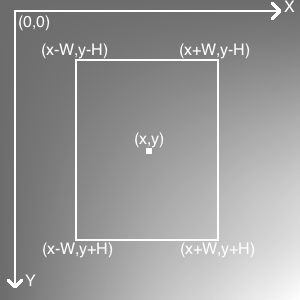
\includegraphics[scale=0.4]{./figs/integral_image}
%     \caption[Ejemplo de Imagen integral]{Ejemplo de Imagen integral: Representación de la ecuación \ref{eq:convolution_in_tree_operations}}
%    \label{fig:integral_image}                %% Etiqueta para la figura entera
% \end{figure}
% 
% \subsubsection{Simetrización}
% Para realizar la convolución a través de los bordes de las imagenes, se debe tener un cuidado especial para que no se produzcan efectos visuales no deseados y por consiguiente la detección de puntos de interés invalidos. Para esto, se consideran condiciones de borde simétricas, es decir que la imagen original es extendida simétricamente hacia cada uno de sus lados utilizando el tamaño del filtro caja más grande antes de calcular la imagen integral como se puede apreciar en la Fig. \ref{fig:symetrized_image}.
% \begin{figure}[tbhp]
%    \centering
%    %%----primera subfigura----
%    \subfloat[]{
%         \label{fig:lena}         %% Etiqueta para la primera subfigura
%         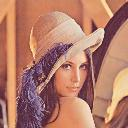
\includegraphics[scale=0.35]{./figs/lena}}
%    \hspace{0.1\linewidth}
%    %%----segunda subfigura----
%    \subfloat[]{
%         \label{fig:symetrized_lena}         %% Etiqueta para la segunda subfigura
%         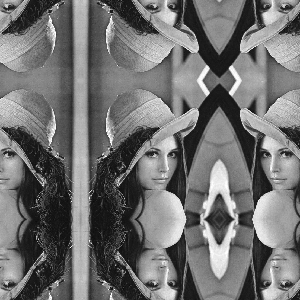
\includegraphics[scale=0.35]{./figs/symetrized_lena}}
%     \caption[Condiciones de borde simétricos para la imagen]{\ref{fig:lena}: Imagen de ``lena'' original. \ref{fig:symetrized_lena}:Imagen de ``lena'' extendida simétricamente}
%    \label{fig:symetrized_image}                %% Etiqueta para la figura entera
% \end{figure}
% 
% \subsubsection{Comparación con el espacio-escala Gaussiano}
% La representación espacio-escala de una imagen $u$ puede ser obtenida mediante la convolución con un kernel gaussiano como se aprecia en \ref{eq:convolution_scalar_space_kernel_gauss}
% \begin{equation}
% \label{eq:convolution_scalar_space_kernel_gauss}
% u_\sigma=g_\sigma * u
% \end{equation}
% donde $g_\sigma$ es el kernel gaussiano 2-D (centrado) que viene definido por \ref{eq:kernel_gaussiano_scale_space} y siendo $\sigma$ el parámetro que representa la escala.
% \begin{equation}
% \label{eq:kernel_gaussiano_scale_space}
% g_{\sigma}(x,y)=\frac{1}{2\pi\sigma^{2}}e^{-\frac{x^{2}+y^{2}}{2\sigma^{2}}}
% \end{equation}
% Haciendo uso de la técnica de filtros caja mencionados, la representación \ref{eq:kernel_gaussiano_scale_space} puede ser aproximada mediante la convolución discreta $\tilde{u}_{\sigma}=B_{L}*u$, donde $B_L$ es el filtro caja con ancho de banda $L$, esto es con un soporte cuadrado $\left[-\frac{L}{2},\frac{L}{2}\right]\times\left[-\frac{L}{2},\frac{L}{2}\right]$. En la configuración discreta, los valores tomados por $L$ son enteros e impares \cite{conf/scalespace/GwosdekGBW11}. Luego, los valores correspondientes a $\sigma$, vienen dados por \ref{eq:sigma_posible_values}.
% \begin{equation}
% \label{eq:sigma_posible_values}
% \sigma\text{\texttwosuperior=\ensuremath{\frac{L\text{\texttwosuperior-1}}{12}}}
% \end{equation}
% Observación: observar que el filtro caja debería ser normalizado por un factor $L^2$ para obtener un kernel cuadrado. Este no es el caso para tomar una consideración en lo que refiere a tiempos de cálculo. Esta normalización es llevada a cabo una sola vez durante el paso de detección de características.
% 
% En las figuras \ref{fig:japan_images} mostradas se puede observar la aproximación de escala-espacio obtenido cuando se usan filtros caja, comparado con la espacio escala lineal obtenida con los kernels gaussianos. Se debe observar que son similares, pero los espacio-escala aproximados exhiben algunos artefactos verticales y horizontales destacados debido a la anisotropía de los kernels caja.
% 
% \begin{figure}[tbhp]
%    \centering
%         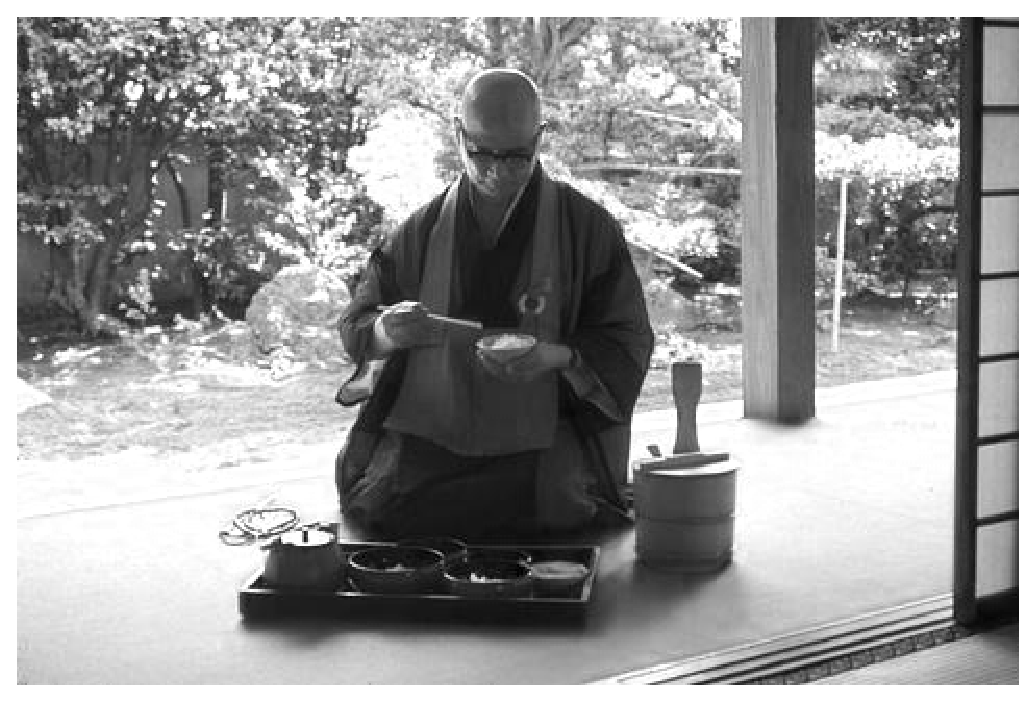
\includegraphics[scale=0.4]{./figs/japan}
%     \caption[Imagen original $u$]{Imagen original $u$}
%    \label{fig:japan_original_image}                %% Etiqueta para la figura entera
% \end{figure}
% 
% \begin{figure}[tbhp]
%    \centering
%    %%----primera subfigura----
%    \subfloat[]{
%         \label{fig:japan_tita}         %% Etiqueta para la primera subfigura
%         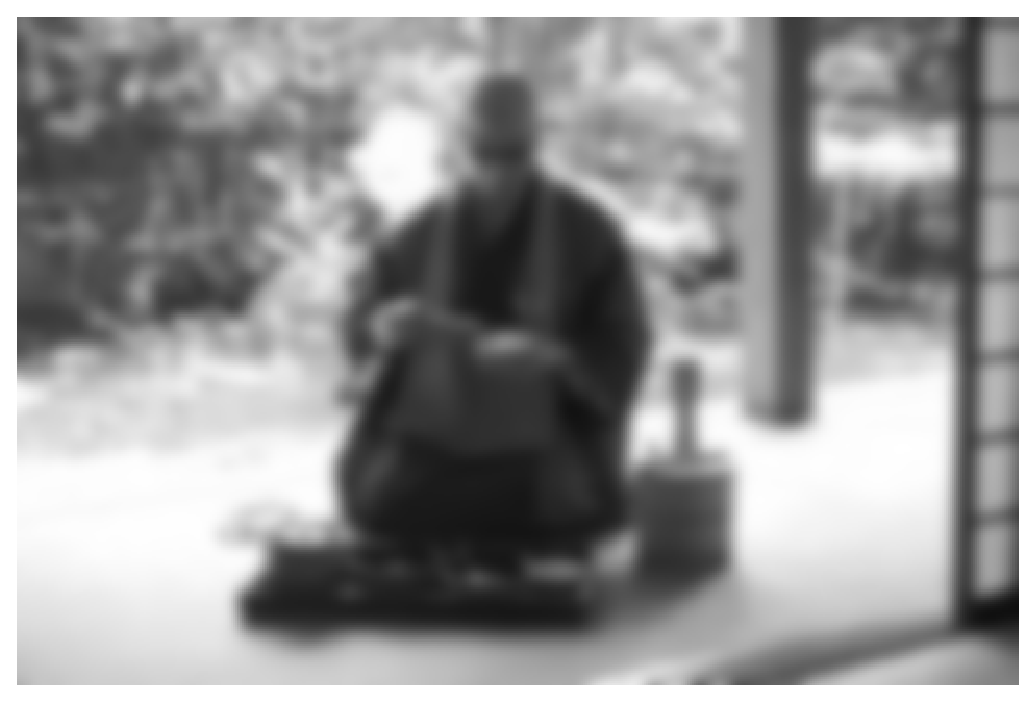
\includegraphics[scale=0.45]{./figs/japan_tita}}
%    %\hspace{0.01\linewidth}
%    %%----segunda subfigura----
%    \subfloat[]{
%         \label{fig:japan_tita_l}         %% Etiqueta para la segunda subfigura
%         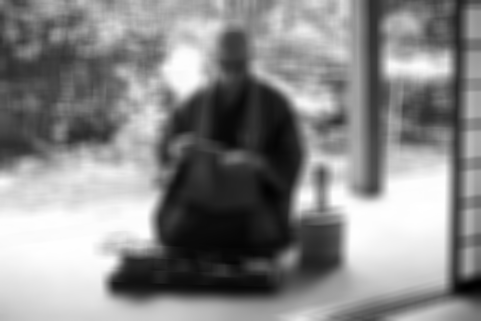
\includegraphics[scale=0.45]{./figs/japan_tita_l}}
%    \hspace{0.1\linewidth}
%    %%----tercera subfigura----
%    \subfloat[]{
%         \label{fig:japan_tita_1}         %% Etiqueta para la segunda subfigura
%         
\includegraphics[scale=0.45]{./figs/japan_tita_1}}
%   % \hspace{0.01\linewidth}
%    %%----cuarta subfigura----
%    \subfloat[]{
%         \label{fig:japan_tita_1_l}         %% Etiqueta para la segunda subfigura
%         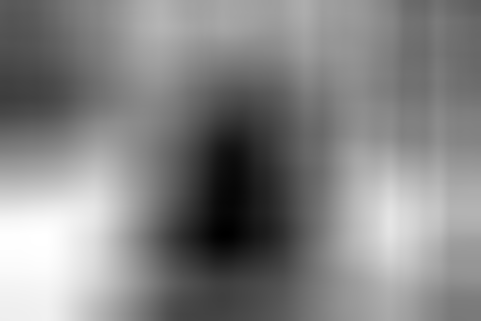
\includegraphics[scale=0.45]{./figs/japan_tita_1_l}}
%   %\hspace{0.01\linewidth}
%     \caption[caption]{Espacio-escala lineal obtenido con los kernels gaussianos y aproximación de espacio-escala cuando se usan filtros caja. (Se ha cambiado el contraste de la imagen para realzar los detalles). \ref{fig:japan_tita} $u_{\sigma}$ con $\sigma=1.708$, \ref{fig:japan_tita_l} $\tilde{u}_{\sigma}$ con $L=13$, \ref{fig:japan_tita_1} $u_{\sigma}$ con $\sigma=14.431$, \ref{fig:japan_tita_1_l} $\tilde{u}_{\sigma}$ con $L=101$}
% \label{fig:japan_images}                %% Etiqueta para la figura entera
% \end{figure}
% 
% Observación: Notar que una mejor aproximación de la escala-espacio puede obtenerse mediante el uso de filtros iterativo caja \cite{conf/scalespace/GwosdekGBW11}, pero el uso de los mismos implican una mayor complejidad.
% 
% \subsubsection{Muestreo escala-espacio}
% Similarmente al algoritmo SIFT, el análisis escala-espacio en SURF esta basado en un muestreo regular del parámetro de escala $\sigma$. La representación de la escala es dividida en \emph{octavas}: una nueva octava corresponde a la duplicación del tamaño del kernel (lo que significa que $\sigma$ sigue una serie geométrica). Cada octava es a su vez dividida en diferentes niveles (o intervalos), cada uno correspondiente al menor incremento del tamaño del filtro discreto involucrado.
% 
% Así definiendo $o$ como el índice que representa la octava e $i$ el índice del intervalo, el muestreo de escala es obtenido mediante la relación \ref{eq:relation_scale_octave}
% \begin{equation}
% \label{eq:relation_scale_octave}
% \sigma=\frac{1.2}{3}(2^{o}\times i+1)=\frac{1.2}{3}\times l,
% \end{equation}
% donde $3l$ es el ancho de banda del filtro caja correspondiente.
% 
% Notar que, contrariamente al método SIFT \cite{Lowe2004}, la imagen no es sub muestreada por un factor de dos en cada octava. No todas las escalas son usadas para seleccionar los puntos de interés y computar los descriptores correspondientes. Las escalas no utilizadas son requeridas para eliminar aquellos valores que no son máximos. Además, contrariamente al enfoque SIFT, el cálculo de la representación escala-espacio en sí no es necesaria, ya que los operadores diferenciales puede también aproximarse utilizando filtros de caja como se explaya a continuación en la sección \ref{subsubsection:approximation_diferential_operators}
% 
% \subsubsection{Aproximación de los operadores diferenciales}
% \label{subsubsection:approximation_diferential_operators}
% Con el objetivo de detectar los puntos interesantes y de construir los descriptores que incrementan los cambios de contraste afín, los operadores diferenciales de primer y segundo orden son calculados en el espacio escala. En la representación lineal espacio-escala, obtenida por la convolución con el kernel gaussiano (como se emplea en SIFT), esto se reduce a calcular la operación de convolución \ref{eq:operation_convolution_aproximation}
% \begin{equation}
% \label{eq:operation_convolution_aproximation}
% D_{\alpha\beta}^{(\sigma)}u_{0}(x,y,\sigma)=(D_{\alpha\beta}g_{\sigma})*u(x,y),
% \end{equation}
% donde $\alpha$ y $\beta$ se refieren a la primera o segunda variable ``x'' e ``y''.
% 
% En el método SURF, este cálculo es aproximado mediante la convolución de una combinación lineal de filtros caja \ref{eq:combination_filter_box}
% \begin{equation}
% \label{eq:combination_filter_box}
% \tilde{D_{\alpha\beta}^{(\sigma)}*u,}
% \end{equation}
% definido en los párrafos siguientes.

% \section{Correspondencia de características entre imágenes}
% \label{sec:correspondencia_caracteristicas_img}
% La correspondencia de características es el proceso en el que los descriptores de los puntos claves de dos o más imágenes son comparados y los pares de correspondencias son creados. Existen muchos métodos para realizar la correspondencia de descriptores de puntos claves. El método más básico está basado en la búsqueda del vecino más cercano entre dos conjuntos de puntos claves. Dadas dos imágenes $I_1$ e $I_2$, el espacio vector n-dimensional se encuentra formado por los descriptores $d(k)$ del conjunto $K1$, $K2$ de puntos claves. Los pares de correspondencias $<k_{i},l_{i}>$ se forman como lo expresa la expresión \ref{eq:correspondence_pairs:expr}
% \begin{equation}
%  \label{eq:correspondence_pairs:expr}
% \forall k_{i}\in K_{1}:l_{i}=\arg\min_{l\in K_{2}}|d(k_{i})-d(l)|
% \end{equation}
% 
% %http://saravananthirumuruganathan.wordpress.com/2010/05/17/a-detailed-introduction-to-k-nearest-neighbor-knn-algorithm/
% % \subsection{esquema de búsqueda en árbol kd}
% % slipa modificado por mi
% % La idea general detrás de los árboles KD se describirá a continuación. Los elementos guardados en el árbol KD son vectores de altas dimensiones en $R^d$. En el primer nivel (la raíz) del árbol, los datos son divididos en dos mitades por un hiper plano ortogonal a una dimensión elegida con un valor de umbral. Generalmente, esta división sea realiza se realiza con la media en la dimensión con la mayor varianza del conjunto de datos. Mediante la comparación del vector de consulta con el ``valor de partición'', es fácil determinar a que mitad de el conjunto de datos del vector de consulta pertenece. Cada una de las mitades de los datos, es luego recursivamente dividida de la misma forma explicada anteriormente para crear un árbol binario completamente balanceado.
% % En la parte inferior del árbol, cada nodo del árbol, corresponde a un punto simple del conjunto de datos, aunque en algunas aplicaciones, los nodos hojas pueden tener más de un punto.
% % La profundidad del árbol resulta ser $log_2 (N)$ donde $N$ es el número de puntos del conjunto de datos.
% 
% % Dado un vector de consulta, un descenso en el árbol requiere $log_2(N)$ comparaciones y el acceso a un nodo hoja del arbol.
% Una vez que han sido identificados los puntos claves y sus descriptores asociados sobre la imagen, % utilizando las herramientas descriptas en la sección %(\ref{extraccion_caracteristicas}), 
% se procede con la búsqueda de correspondencia (en caso de existir) entre la imagen de entrenamiento o patrón y la imagen del flujo de vídeo. De esta forma se busca identificar si el objeto se encuentra presente en la imagen capturada.
% 
% Como se ha visto, un descriptor SURF es un vector de 64 dimensiones que caracteriza localmente una vecindad de un punto clave. Generalmente, gran cantidad de descriptores SURF son extraídos de la imagen y la consulta consiste en buscar los vectores que mejor coincidan, tarea que no resulta trivial a la hora de lograr tiempos de ejecución acotados.
% Existen diversas técnicas, para dar respuestas a este problema. Una de más mencionadas es la denominada \textit{búsqueda del vecino más cercano} (del ingl\'es, Nearest Neighbor Search o NNS) \cite{AryaEtAl98} y sus variantes.

% \subsection{Búsqueda del vecino más cercano}
% El m\'etodo de búsqueda del vecino más cercano es de utilidad en gran variedad de aplicaciones como el reconocimiento de imágenes, la compresión de datos, el reconocimiento de patrones y su clasificación, el aprendizaje máquina, los sistemas de recuperación de documentos, estadísticas y análisis de datos, entre otros. 
% 
% Es un problema de optimización que intenta buscar los puntos más cercanos en un espacio métrico. Éste, puede definirse de la siguiente forma: dado un conjunto de puntos $P=\left\{ p_{1,...,}p_{n}\right\}$ en un espacio métrico $M$ y un punto de consulta $q \in M$, encontrar el/los punto/s más cercano/s a $q$ en $P$ donde $M$ es un espacio euclídeo d-dimensional y las distancia es medida mediante la distancia euclídea o Manhattan. 

% Resolver este tipo de problemas no resulta trivial en espacios de grandes dimensiones. No es usual encontrar algoritmos que posean un rendimiento mayor al de la búsqueda lineal (también conocida como ``búsqueda por fuerza bruta''), la cual resulta ser muy costosa y a veces inaplicable para muchas aplicaciones. Es por esto, que se ha generado un gran interés en algoritmos \footnote{\url{http://www.cs.umd.edu/~mount/ANN/}} que puedan realizar la búsqueda del vecino más cercano de forma aproximada, con lo cual es posible lograr mejoras significativas en tiempo de ejecución con errores de precisión relativamente pequeños y aceptables \cite{Beis:1997:SIU:794189.794431}.

% \subsubsection{Remoción de pares irrelevantes}
% Esta aproximación tiene la desventaja que la correspondencia se genera para cada $k_i$, independientemente de que las características sean muy similares, debido a que siempre se encuentra un vecino cercano. Lowe \ref{Lowe2004} propone usar un ratio para rechazar pares de puntos claves no especificos. La distancia euclidea $d1$, $d2$ de dos vecinos más cercanos es comparada y si el ratio cumple $\frac{d_{1}}{d_{2}}>\varepsilon\qquad(\varepsilon=0.8\:\ref{Lowe2004})$, el par de correspondencias es desechado. Esto rechaza todos los puntos claves, para los cuales no hay una correspondencia especifica en la segunda imagen.
% 
% En muchos casos el objeto plano buscado contiene muchas características genericas como esquinas o simples curvas. Este problema ocurre comunmente cuando se buscan locos o simple logos. Estas características pueden ser encontradas muchas veces en la imágen objetivo y pueden producir que no se encuentre la homografía correcta. Esta remoción reduce el numero de pares dispnibles para buscar la correspondencia, pero realza la habilidad de buscar la homografía correcta mediante la reducción de correspondencias incorrectas.

% \section{Correspondencia de los puntos claves}
% 
%  \subsection{Indexación rápida}
% %ESTO NO SE USA!! : PORQUE SEG;UN LO QUE ME MANDO MARIUS MUJA EN EL MAIL DICE QUE DIVIDIR SEGUN EL SIGNO ES MUCHO MAS LENTO Y LOS RESULTADOS NO SON APRECIABLES.
%  Comúnmente, los puntos claves detectados, se hallan en regiones y puntos que difieren en intensidad de su vecindad. El signo del Laplaciano (por ejemplo la traza de la matriz hessiana) distingue regiones de claras (alta luminosidad) de fondos oscuros (baja luminosidad) y viceversa. Este dato está disponible sin un costo computacional extra debido a que ya ha sido calculada en la fase de detección descripta en la Sec. \ref{sec:matHessiana}. Así, en la etapa de búsqueda de correspondencias, solo se comparan las características si el ``contraste'' entre ellas es similar, véase la figura \ref{fig:contrastcomparation} como un ejemplo. Esta información resulta ventajosa para métodos de indexación como kd-trees definiendo un hiper plano para dividir los datos, opuesto a seleccionar un elemento aleatoriamente o usar estadísticas de características.
% 
%     \begin{figure}[tbhp]
%       \centering
% 	    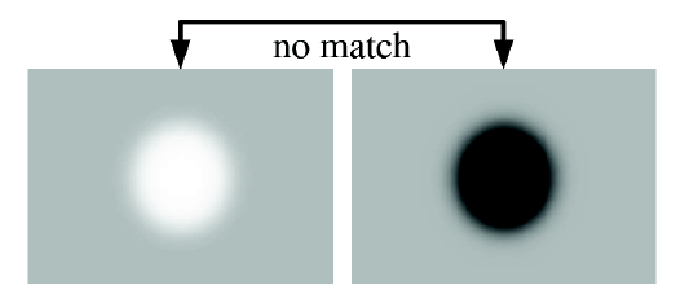
\includegraphics[scale=0.4]{./figs/notmatching}
% 	\caption[]{Si el contraste entre dos puntos de interés es diferente (oscuro sobre fondo claro versus claro sobre fondo oscuro), el candidato no es considerado como una coincidencia valiosa.)}
%       \label{fig:contrastcomparation}
%     \end{figure}

 %Este umbral puede ser interpretado como: Un par es detectado como coincidente si la distancia es lo suficientemente cercana a $n$ veces la distancia del segundo más cercano. 
   \chapter{Fundamentos teóricos}
\label{c:parte3}
\vspace{1cm}
En este capítulo, se presentan los fundamentos teóricos sobre los cuales se sustenta el proyecto y particularmente el método luego utilizado. Primeramente se describen algunas operaciones morfológicas sobre imágenes y algunas técnicas de realce sobre las mismas. Tras ello, se explica un método de detección y descripción de características en imágenes. También, se presenta una técnica para búsqueda de correspondencias entre puntos característicos de imágenes, que sirve como base para encontrar la relación entre dos imágenes de un mismo objeto fotografiado desde diferentes perspectivas.
\section{Operaciones morfológicas en imágenes}
El procesamiento morfológico en imágenes es un tipo de procesamiento en el cual la forma espacial o estructura de los objetos en la imagen es modificada. La erosión y dilatación son dos operaciones morfológicas fundamentales que pueden ser aplicadas a imágenes en escala de grises o imágenes binarias. En esta sección se describen tanto la erosión como la dilatación enfocándose en imágenes binarias que son las utilizadas en este trabajo.

El lenguaje de la morfología matemática es el de la teoría de conjuntos y la misma representa objetos en las imágenes. Por ejemplo, el conjunto de todos los píxeles negros en una imagen binaria es una descripción morfológica completa de la imagen. En imágenes binarias, el conjunto en cuestión es miembro de un espacio entero 2-D $Z^2$, donde cada elemento del conjunto es una tupla (vector 2-D) cuyas coordenadas son las coordenadas $(x,y)$ de un píxel negro (o blanco, dependiendo de la convención) de la imagen.

A continuación, definiremos algunas notaciones que serán utilizadas para definir posteriormente la erosión y la dilatación: nos referiremos con $A$ a un conjunto en $Z^2$, $a=(a_1,a_2)$ un elemento de $A$, $\varnothing$ un conjunto vacío, $A \subseteq B$ para denotar que $A$ es un subconjunto de $B$,  $A \cap B$ para indicar la intersección entre $A$ y $B$ (el conjunto de elementos que corresponde tanto a $A$ como a $B$), $\hat{B}=\{w|w=-b, \; \textrm{para} \; b \in B\}$ para indicar la reflexión del conjunto $B$,  $(A)_{z}=\{c|c=a+z,\; \textrm{para}\; a \in A\}$ para indicar la traslación del conjunto $A$ por $z=(z_1, z_2)$ y $\{\cdot\}$ la notación de un conjunto.
\subsection{Dilatación}
Sea $A$ y $B$ un conjunto en $Z^2$, la dilatación entre $A$ y $B$ denotada como $A \oplus B$ queda definida como
\begin{equation}
A\oplus B=\{z|(\hat{B})_{z}\cap\; A \neq \varnothing\},
\label{eq:eq_dilatacion}
\end{equation}
%De la expresión \ref{eq:eq_dilatacion}, se puede decir que la dilatación se basa en obtener la reflexión de $B$ sobre su origen y tras ello hace una traslación por $z$. 
donde $B$ comúnmente es conocido como máscara o kernel.

Mediante la dilatación, los objetos crecen en su tamaño y algunos de los ``espacios'' dentro de ellos son rellenados. Un ejemplo de dilatación sobre la imagen de la Fig. \ref{fig:original_erode_dilate} utilizando el kernel de la Fig. \ref{fig:mascara}, se puede observar en la Fig. \ref{fig:dilatacion_example} (se realizaron 2 dilataciones para resaltar el efecto de la operación).
% \begin{figure}[tbhp]
%    \centering
%         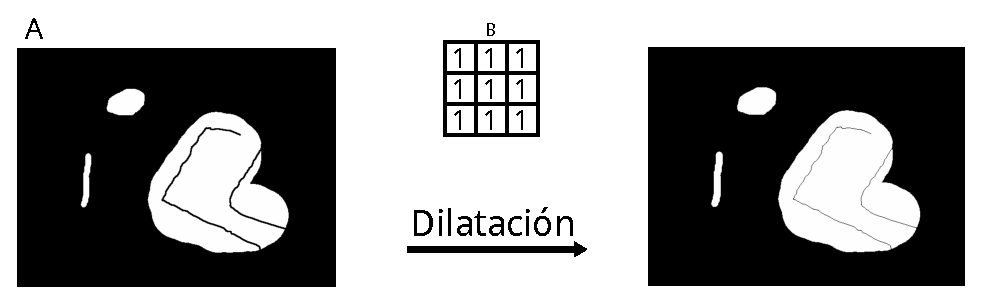
\includegraphics[scale=0.75]{../figs/dilatacion_example}
%      \caption[Dilatación de una imagen]{}
%    \label{}                %% Etiqueta para la figura entera
% \end{figure}
\subsection{Erosión}
Sea un conjunto $A$ y $B$ de $Z^2$, la erosión de $A$ por $B$, denotada como $A \ominus B$ queda definida como
\begin{equation}
A \ominus B=\{z|(B)_{z} \subseteq A\}.
\label{eq:eq_erosion}
\end{equation}
De la ecuación \eqref{eq:eq_erosion} se puede interpretar que la erosión de $A$ por $B$ es el conjunto de todos los puntos $z$ tales que $B$, trasladados por $z$, están contenidos en $A$.

Uno de los usos más simples de la erosión es la eliminación de detalles irrelevantes (en términos de tamaño) de una imagen binaria. En una imagen erosionada, el tamaño de los objetos se ve reducido y el ruido o detalles irrelevantes (aislados) es eliminado. Un ejemplo de erosión sobre la imagen de la Fig. \ref{fig:original_erode_dilate} utilizando el kernel de la Fig. \ref{fig:mascara}, se puede observar en la Fig. \ref{fig:erosion_example} (se realizaron 2 erosiones para resaltar el efecto de la operación).
% \begin{figure}[tbhp]
%    \centering
%         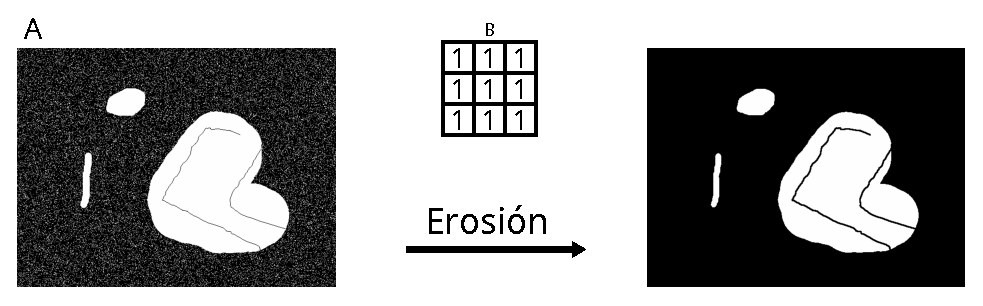
\includegraphics[scale=0.75]{../figs/erosion_example}
%     \caption[Erosión de una imagen]{Erosión de una imagen con una máscara (B) de $3\times3$.}
%    \label{fig:erosion_example}                %% Etiqueta para la figura entera
% \end{figure}
% % 
% Los filtros morfológicos son operadores que transforman una imagen de una forma predefinida (de acuerdo a la forma de la máscara aplicada). La interacción entre el filtro y los vecinos al píxel sobre el cuál se está aplicando el procesamiento, dan el resultado final de la transformación.
% 
% Técnicas como erosión, dilatación, entre otras, son algunas clases de este tipo de operaciones que poseen muchas aplicaciones y que en ocasiones son parte de un pre-procesamiento sobre las imágenes, para su posterior tratamiento con el objetivo de detectar una zona sobre la cual aplicar el procesamiento o eliminar zonas que resulten irrelevantes.
% 
% \subsection{Erosión y dilatación}
% Las erosión y dilatación son dos operaciones morfológicas usadas en variedad de contextos como remoción de ruido, aislación/unión de elementos, etc.
% 
% 
% 
% % Estos dos filtros operan sobre un conjunto de píxeles vecinos alrededor de cada píxel de la imagen sobre la cual es aplicada la operación.
% 
% La \emph{erosión}, reemplaza al píxel actual con el valor mínimo de la vecindad definida mediante un kernel, mientras que la \emph{dilatación} es la operación complementaria a la anterior, es decir, que reemplaza el píxel actual con el valor máximo del conjunto de píxeles vecinos definidos mediante el kernel. Así, en el caso de una imagen binaria (sólo contiene píxeles negros o blancos representados en nuestro caso con el valor 0 y 255), cada píxel es reemplazado por uno negro o blanco.  En el caso de la dilatación, los objetos crecen en su tamaño y algunos de los espacios dentro de ellos son rellenados.
% 
% % Una buena forma de ver el efecto de este operador es en términos de una imagen con fondo negro y objetos blancos. Cuando se aplica la erosión, si un píxel del filtro aplicado esta sobre el fondo, luego el píxel sobre el cuál se esta aplicando la erosión resultará con el valor del fondo. Mientras, que en el caso de la dilatación, si el filtro toca un objeto sobre el fodno, el pixel será asignado al valor del blanco. 
% % poner que máscara se usa y poner imagen
% % cvErode(frameDiferencia, frameDiferencia, NULL, 2);
% % cvDilate(frameDiferencia, frameDiferencia, NULL, 2);
% %http://opencv.willowgarage.com/documentation/miscellaneous_image_transformations.html?highlight=cvthreshold#cvThreshold
\begin{figure}[tbhp]
\centering
\subfloat[][Imagen sobre la que se realizan las operaciones (Figura tomada de \cite{Gonzalez:02}).]{
\includegraphics[width=2.3in]{../figs/erode_dilate/orig} \label{fig:original_erode_dilate}}  \qquad
\subfloat[][Kernel o máscara de $3\times3$.]{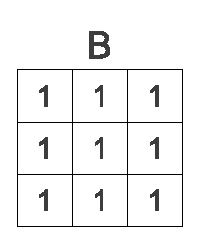
\includegraphics[width=1.0in]{../figs/mascara} \label{fig:mascara}}\\
\subfloat[][Dilatación ($\times$2).]{
\includegraphics[width=2.3in]{../figs/erode_dilate/2dilate} \label{fig:dilatacion_example}}
\subfloat[][Erosión ($\times$2).]{
\includegraphics[width=2.3in]{../figs/erode_dilate/2erode} \label{fig:erosion_example}}
\caption[Efecto de la operación de erosión y dilatación sobre una imagen]{Efecto de la operación de erosión y dilatación sobre la imagen \subref{fig:original_erode_dilate}. \subref{fig:mascara} Máscara o kernel utilizado para cada una de las operaciones. \subref{fig:dilatacion_example} Resultado de aplicar la dilatación ($\times2$). \subref{fig:erosion_example} Resultado de aplicar la erosión ($\times2$).
}
\end{figure}
\section{Realce de imágenes en el dominio espacial}
\label{subsec:mejoras_iluminacion}
En esta sección se presentan brevemente algunas técnicas en el dominio espacial. Las mismas, fueron seleccionadas debido a que presentan tiempos de cálculo pequeños y son orientadas a la tarea de realce de detalles o mejora de la iluminación en las imágenes.

Los métodos en el dominio espacial son procedimientos que operan directamente sobre los píxeles de la imagen y pueden denotase con la expresión $g(x,y)=T[f(x,y)]$, donde $f(x,y)$ es la imagen de entrada, $g(x,y)$ es la imagen resultado de la operación y $T$ es un operador sobre $f$ definido sobre alguna vecindad alrededor de $(x,y)$ \cite{Gonzalez:02}. 

El enfoque principal en la definición de la vecindad alrededor de un punto $(x,y)$, es el uso de una zona de sub imagen cuadrada o rectangular centrada en $(x,y)$. Cuando esta vecindad se establece a un valor de $1 \times 1$ (un píxel), $g$ depende únicamente del valor de $f$ en $(x,y)$ y $T$ se convierte en una función de transformación de intensidad de la forma $s=T(r)$. Dado que en este proyecto se trabaja con imágenes en escala de grises, $r$ y $s$ son variables que denotan el nivel de gris de $f(x,y)$ y $g(x,y)$ en el punto $(x,y)$ respectivamente.
\subsection{Umbral}
Podemos definir una función de umbral como una transformación con la forma de la expresión \eqref{eq:equation_umbral_binario} donde $r_{max}$ y $s_{max}$ son los valores máximos de intensidad de la imagen $f(x,y)$ y $g(x,y)$ respectivamente y $u$ una constante que define el valor de umbral de la transformación.

La función de umbral particular presentada en la Fig. \ref{fig:umbral_curve} produce una imagen binaria asignando el valor $s_{max}$ a los valores que superan $u$ y $0$ a los demás.
\begin{equation}
\label{eq:equation_umbral_binario}
s= 
\begin{cases} 0 & \text{para $r<u$,}
\\
s_{max} &\text{para $r>=u$}
\end{cases} \textrm{con } 0 \leq r \leq r_{max} \textrm{ y } 0 \leq u \leq r_{max}.
\end{equation}

\begin{figure}[tbhp]
   \centering
        \includegraphics[scale=1.0]{../figs/iluminacion/umbral}
    \caption[Umbral binario]{Umbral binario.}
   \label{fig:umbral_curve}                %% Etiqueta para la figura entera
\end{figure}
%cvThreshold (50, 255, CV\_THRESH\_BINARY) y agregar grafico del umbral
% \bigskip
% \textbf{Referencias de la sección: \cite{citeulike:3484001}, %Gary Bradsky et al., 2008 
% \cite{citeulike:9456628}, %Robert Laganière, 2011
% \cite{bb1919}. %D. Conrad et al., 2010 
% }
\subsection{Transformación logarítmica}
\label{subsec:transf_logaritmica}
Esta transformación viene expresada por la ecuación \eqref{eq:logaritmo}, donde $s$ es el valor resultante de aplicar la transformación sobre el valor de entrada $r$ (con $r \geq 0$) y $c$ es una constante, que en la práctica comúnmente se establece como $c=1$. Utilizada cuando la imagen de entrada tiene un rango dinámico grande, expande las intensidades oscuras y comprime las intensidades claras como se puede observar en la curva de la Fig. \ref{fig:log_curve}.
\begin{equation}
    s=c\;log(1+r).
    \label{eq:logaritmo}
\end{equation}
\begin{figure}[tbhp]
   \centering
        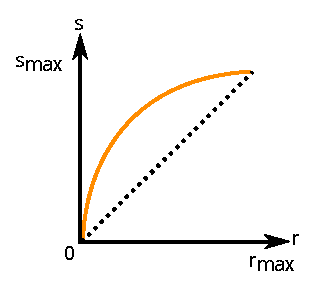
\includegraphics[scale=1.0]{../figs/iluminacion/logaritmo}
    \caption[Curva de la transformación logarítmica]{Curva de la transformación logarítmica.}
   \label{fig:log_curve}                %% Etiqueta para la figura entera
\end{figure}
\subsection{Ecualización de histograma}
\label{subsec:iluminacion_ecualizacion}
El histograma es una función discreta que describe de manera global la apariencia de una imagen y puede ser interpretada como el número de píxeles en función de las intensidades de grises.

La ecualización del histograma de una imagen de grises es una transformación que pretende obtener el mismo número de píxeles para cada nivel de gris de la imagen, logrando obtener así un histograma con una distribución que se aproxima a la uniforme. Como resultado de esta transformación global que redistribuye los grises de la imagen original para que abarque una gama más completa de los grises disponibles, se obtiene una expansión en el rango dinámico de la imagen.

Si se tienen imágenes digitales (valores discretos) con intensidades entre 0 y 1, y sea:
\begin{itemize}
 \item $n$ la cantidad de píxeles de la imagen,
 \item $p$ el número de bits de resolución de la imagen,
 \item $L$ el máximo nivel de gris, dado por el valor de $p$,
 \item $k$ el nivel de gris,
 \item $r_k$ el nivel de gris normalizado a 1, con valores $r_{k}=0,\frac{1}{2^{p}-1},\frac{2}{2^{p}-1},\ldots,1.$
 \item $p_{r}(r_{k})$ la probabilidad de un nivel de gris en la imagen calculado como:
\end{itemize}
\begin{equation}
p_{r}(r_{k})=\frac{n_{k}}{n},\; \textrm{con}\begin{cases}
\begin{array}{c}
0\leq r_{k}\leq1\\
k=0,1,\ldots,L-1
\end{array},\end{cases}\label{eq:relacion_probabilidades}
\end{equation}
la función de transformación utilizada es la Función de Distribución Acumulada:% que se expresa en la ecuación \eqref{eq:cdf_acumulada}.
\begin{equation}
s_{k}(r_{k})=T(r_{k})=\sum_{j=0}^{k}\frac{n_{j}}{n}=\sum_{j=0}^{k}p_{r}(r_{j}),\; \textrm{con}\begin{cases}
\begin{array}{c}
0\leq r_{k}\leq1\\
k=0,1,\ldots,L-1
\end{array}.\end{cases}\label{eq:cdf_acumulada}
\end{equation}
\subsection{Filtrado pasa altos}
\label{suubsec:iluminacion_pasaaltos}
Los filtros pasa altos realzan las altas frecuencias que son los detalles de una imagen y pueden ser realizados mediante una diferenciación espacial. La aplicación de este tipo de filtros, realza ejes, bordes y diversas discontinuidades (incluido el ruido) y atenúa áreas cuyos niveles de grises varían lentamente (bajas frecuencias).
% En la práctica las imágenes capturas por lo general presentaban el efecto de borroneado en algunos casos.

Un filtro pasa altos puede ser aplicado mediante la convolución de la imagen con un kernel pasa altos que puede ser de diferentes tamaños y que según esto, actuará de diferentes maneras (realzando en mayor o menor medida los detalles). Si definimos a $f(x+s, y+t)$ como el valor de los píxeles del bloque seleccionado de la imagen y $w(s,t)$ los coeficientes del kernel, se puede expresar el filtrado lineal con la expresión definida en la ecuación \eqref{eq:ec_convolucion}.
\begin{equation}
g(x,y)=\sum_{s=-a}^{a}\sum_{\; t=-b}^{a}w(s,t)f(x+s,y+t).\label{eq:ec_convolucion}
\end{equation}

Si la suma de los coeficientes del kernel es 1, se realzan las altas frecuencias conservándose el brillo medio de la imagen sobre la cual se aplica el filtro.
\subsection{Filtrado de alta potencia}
\label{subsec:iluminacion_altapotencia}
El filtrado de alta potencia es una generalización del filtro de máscara difusa y se obtiene mediante la diferencia entre una versión amplificada de la imagen original y una versión suavizada de la misma.

Sea una constante $A \geq 1$, $f(x,y)$ la imagen sobre la cual aplicaremos el filtrado de alta potencia, $PB(f(x,y))$ el resultado de aplicar un filtro pasa bajos a la imagen $f(x,y)$ y $g(x,y)$ el resultado de la operación, el filtrado de alta potencia queda definido como en la ecuación \eqref{eq:form_alta_potencia}. En el caso particular de establecer el valor $A=1$, se obtiene un filtrado pasa altos.
\begin{eqnarray}
\label{eq:form_alta_potencia}
\begin{aligned}
  g(x,y)&=Af(x,y)-PB(f(x,y))\\
  &= (A-1)f(x,y)+PA(f(x,y)).
\end{aligned}
\end{eqnarray}
\section{Detección de puntos claves}
  \label{sec:detec_ptos_claves}
  En visión computacional, el concepto de puntos de interés es ampliamente usado como se ha descripto en la Sec. \ref{sec:ptos_caract_descriptores}. El método SURF fue desarrollado por Herbert Bay et. al \cite{Bay:2008:SRF} como un detector y descriptor robusto de puntos.
  
%%%%%%%%%%%%%%%%%%%%%%%%%%%%%%%%%%%%%%%%%%%%%%%%%%%%%%%%%%%%%%%%%%%%%%%%%%%%%%%%%
  La selección del detector SURF, se ve fundamentada por ser un detector y descriptor de puntos de interés rápido, invariante a escala (concepto que será descripto en la Sec. \ref{sec:invarianza_a_escala}) y rotación que provee ganancia en velocidad debido al uso de imágenes integrales \cite{Bay:2008:SRF}. Este tipo de imágenes permite reducir drásticamente el número de operaciones para convoluciones con los filtros tipo caja, independientemente del tamaño de escala. Además, SURF utiliza una aproximación a la matriz hessiana para la detección de puntos de interés la cual resulta comparable con los detectores de puntos de interés del estado del arte, o aún incluso, se obtiene mejores resultados en ciertos casos \cite{Bay:2008:SRF}. %Incluso sin realizar ningún tipo de optimización, un cálculo casi en tiempo real sin pérdida de rendimiento es posible, lo que representa una ventaja importante para muchas aplicaciones en linea de visión por computador.
  En lo que respecta al descriptor, al estar basado en la suma de las componentes de las Wavelets Haar, la naturalidad de descripción del patrón de intensidad subyacente a la imagen resulta ser más distintiva que los enfoques basados en histogramas. %Además, la simplicidad y el uso de las imágenes integrales, hacen al descriptor competitivo en términos de velocidad .

  SURF, se basa en las ideas planteadas en el método denominado SIFT, pero con algunas diferencias que se presentan resumidas a continuación:
        \begin{itemize}
	\item SURF posee una velocidad de cálculo superior sin perder rendimiento de manera considerable, ésto es logrado mediante la reducción en la dimensión de los vectores descriptores y reduciendo la complejidad de cálculo en los mismos mediante el uso de imágenes integrales \cite{Viola01rapidobject} y filtros tipo caja (del inglés, Box filters)\cite{Simard99boxlets:a},
	\item la gran velocidad de cálculo resulta ser un factor positivo, a pesar de una tolerable pérdida de robustez,
	\item el cálculo de la posición y la escala de puntos claves se realiza utilizando una aproximación a la matriz hessiana (que se detallará en la Sec. \ref{sec:matHessiana}), %  SIFT también detecta características como máximos locales en el espacio imagen y escala, pero usa las respuestas del filtro Laplaciano, en vez de el Determinante Hessiano. Este Laplaciano es calculado a diferentes escalas usando el filtro de Diferencia de Gaussianos. Como el cálculo de los puntos claves esta basado en Kernels de punto flotante, el algoritmo SIFT, es considerado generalmente más preciso que SURF en términos de localización de las características en el espacio imagen y escala, pero resulta computacionalmente más costoso.
	\item utiliza siempre la imagen original para el análisis del espacio escala, a diferencia de SIFT que realiza un redimensionamiento de la imagen en cada paso,
	\item la longitud de los vectores característicos para SURF es la mitad que para SIFT (64 y 128 valores, respectivamente).
       \end{itemize}
  \subsubsection{Imágenes integrales}
      \label{sec:imagenes_integrales}
      Las imágenes integrales \cite{Viola01rapidobject} permiten calcular más rápidamente la convolución con filtros tipo caja. La imagen de entrada $\mathit{I_{\sum}(\mathbf{x})}$ en la posición $\mathbf{x}=(x,y)^{T}$ representa la suma de todos los píxeles de la imagen de entrada $\mathit{I}$ dentro de una región rectangular formada por el origen y $\mathbf{x}$.
%       Una imagen integral $I_{\sum}(\mathbf{x})$ es una imagen en la que el valor del píxel $p=(x,y)$ es la suma de todos los valores de los píxeles entre $p$ y el origen, expresado por la ecuación \ref{eq:integral_image_1}
      \begin{equation}
      \label{eq:integral_image_1}
      \mathit{I}_{\sum}(\mathbf{x})=\sum_{i=0}^{i\leq x}\quad\sum_{j=0}^{j\leq y}I(i,j).
      \end{equation}

      Una vez que la imagen integral se ha calculado, son necesarias tres sumas y cuatro operaciones de acceso a memoria para calcular la suma de las intensidades sobre cualquier área rectangular vertical independientemente de su tamaño (veáse la Fig. \ref{fig:integral_image_sum}). El tiempo de cálculo resulta independiente del tamaño del filtro, lo cual es favorable en la aproximación de SURF en la que se utilizan filtros de grandes tamaños.
      \begin{figure}[tbhp]
	\centering
	      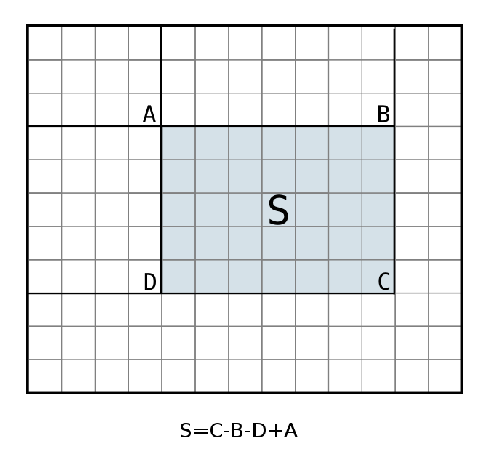
\includegraphics[scale=0.6]{./figs/sumintegralimages2}
	  \caption[Suma de intensidades usando imágenes integrales]{Suma de intensidades en un rectángulo usando imágenes integrales.}
	\label{fig:integral_image_sum}                %% Etiqueta para la figura entera
      \end{figure}

%       La utilización de esta técnica, resulta en un algoritmo invariante a tiempos de cálculo ante cambios del tamaño del filtro, lo cual lo hace particularmente útil cuando se presentan imágenes de grandes dimensiones.   
  En las secciones siguientes, se presenta en detalle los pasos mediante los que se lleva a cabo la detección y descripción de características mediante SURF, introduciendo brevemente el concepto de invarianza a escala.
  \subsection[El problema de cambio de escala]{El problema de cambio de escala en correspondencias de puntos}
    \label{sec:problema_cambio_escala}
    Cuando se trata de hacer coincidir características entre imágenes (por ejemplo para el reconocimiento de las mismas), el problema del cambio de escala se hace presente. Al ser analizadas distintas imágenes, éstas pueden estar tomadas a diferentes distancias respecto del objeto de interés, de forma que los objetos aparecen de diferentes tamaños en la imagen. Luego, si se trata de hacer coincidir las mismas características entre dos imágenes usando un tamaño fijo de píxeles vecinos, la intensidad de los patrones no coincidirá debido al cambio de escala presente en las mismas y por lo tanto, el reconocimiento fallará.

    Para solucionar este problema, el concepto de características invariantes a la escala es introducido en visión computacional, en el que la idea central radica en tener un factor de escala asociada con cada punto clave detectado.
    
    Para comprender mejor esta situación, en la Fig. \ref{fig:church_difference_surf} se presenta un ejemplo de puntos claves detectados con el método SURF. Si se considera la parte inferior de la ventana superior derecha de la fotografía, tanto en la Fig. \ref{fig:church1} como en la Fig. \ref{fig:church2}, la característica SURF ha sido detectada en la misma ubicación y los círculos correspondientes (de diferentes tamaños) contienen los mismos elementos visuales. En la Fig. \ref{fig:church1} la cámara se encuentra más cerca de la escena y el círculo marcado con la flecha roja posee la misma información visual que en la Fig. \ref{fig:church2} donde la escena fue capturada a diferente escala (alejándose la cámara de la escena). % El cambio del tamaño de los círculos correspondientes en ambas imágenes resulta proporcional al cambio de escala. 
    Si bien, en este caso no se da para todas las características, la razón de repetición es lo suficientemente alta para permitir buenas coincidencias entre las dos imágenes. Además, como información adicional, se puede observar una línea radial dentro de cada círculo que indica una orientación asignada a cada punto.% confiriendo invarianza a rotación.
  \subsubsection{Invarianza a escala}%http://fierdetregauche.wordpress.com/2011/03/28/espacio-escala-en-imagenes/
      \label{sec:invarianza_a_escala}
      Es sabido que los filtros gaussianos son comúnmente usados para detección de puntos \cite{Bay:2008:SRF}. Si la escala del filtro es muy pequeña, el resultado incluye muchos puntos redundantes de detalles innecesarios. Contrariamente, si la escala es muy grande, los puntos de regiones con soporte pequeño tienden a desaparecer con el borroneado. Luego, para solucionar los problemas existentes en el filtrado gaussiano con escalas fijas, se han propuesto procedimientos espacio-escala basados en la representación de la curvatura discreta multi escalar. El esquema está basado en el criterio de estabilidad que establece que la presencia de una esquina debe ocurrir como un máximo de curvatura observable en la mayoría de las escalas \cite{springerlink:10.1023/A:1008045108935}.

      La derivada de una imagen puede ser estimada mediante el uso de filtros gaussianos. Los mismos utilizan un parámetro $\sigma$ que representa la varianza de la función gaussiana usada para construir el filtro y que define implícitamente la escala en que la derivada es evaluada.

      Si se calcula el laplaciano de un punto en una imagen usando filtros gaussianos a diferentes escalas, se obtienen diferentes valores en los que se puede observar la evolución de las respuestas para diferentes factores de escala. Así, se  obtiene una curva que alcanza un valor máximo en algún valor de $\sigma$ específico. Si se extrae este valor para dos imágenes del mismo objeto (tomadas a escalas diferentes), la relación que existe entre los $\sigma$ máximos se corresponderán en relación con las escalas en que fueron tomadas cada una de las fotografías. Esta observación es el núcleo del proceso de extracción de características invariantes a la escala que es aplicado tanto en SIFT como en SURF. %Es decir, que las características invariantes a escalas, pueden ser detectadas como máximos locales en ambos espacios. %: espacial (en la imagen) y el espacio escala obtenido de la aplicación de filtros a diferentes escalas.
  \begin{figure}[tbhp]
	\centering
	%%----primera subfigura----
	\subfloat[]{
	      \label{fig:church1}         %% Etiqueta para la primera subfigura
	      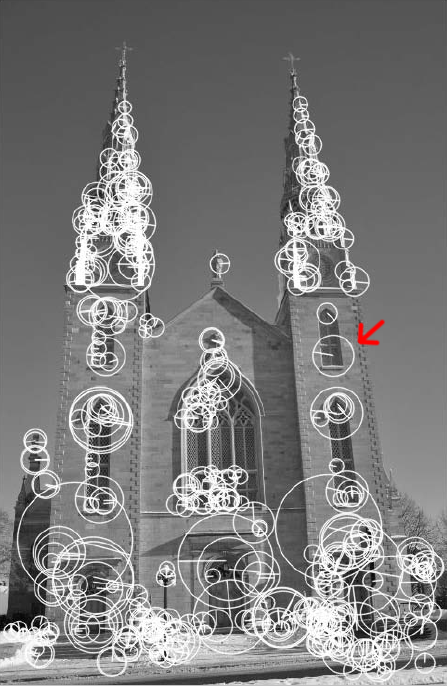
\includegraphics[scale=0.338]{../img_ent2/surfinchurch1}}
	\hspace{0.1\linewidth}
	%%----segunda subfigura----
	\subfloat[]{
	      \label{fig:church2}         %% Etiqueta para la segunda subfigura
	      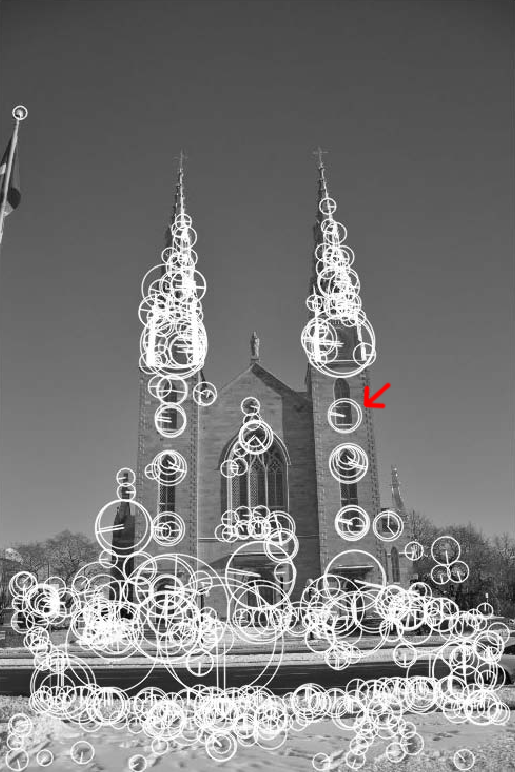
\includegraphics[scale=0.3]{../img_ent2/surfinchurch2}}
	  \caption[Fotografía tomada a diferentes escalas para la misma escena]{Fotografía tomada a diferentes escalas de la misma escena. El tamaño de los círculos de cada punto clave detectado es proporcional a la escala calculada para cada uno de ellos. (Figuras tomadas de \cite{citeulike:9456628}).}
	\label{fig:church_difference_surf}                %% Etiqueta para la figura entera
      \end{figure}
  \subsection{Puntos claves basados en la matriz hessiana}
      \label{sec:matHessiana}
      Con la idea que se introdujo en la sección \ref{sec:problema_cambio_escala}, el descriptor SURF hace uso de la matriz hessiana \eqref{eq:HessianMatrix} y describe cómo las intensidades de los píxeles se distribuyen dentro de una vecindad, que es dependiente de la escala de cada punto de interés detectado por el hessiano. Más específicamente, utiliza el determinante de la matriz para la determinación de la localización y escala de los puntos. Así, cuando el determinante del hessiano es un máximo local (previa eliminación de mínimos mediante un umbral), se determina un punto clave. El uso del hessiano es alentado por su velocidad de cálculo y precisión.%este es el thresholdumbral usado en la funcion %Se puede interpretar que esta matriz mide la curvatura local de una función, mientras que el determinante de la misma da idea de la intensidad que posee la curvatura.
%       La idea es por lo tanto, definir esquinas de imágenes como puntos con con alta curvatura local (esto es, alta variación en más de una dirección)
      \begin{equation}
	H(x,y)=\begin{bmatrix}\frac{\partial^{2}I}{\partial x\text{\texttwosuperior}} & \frac{\partial^{2}I}{\partial x\partial y}\\
	& \\
	\frac{\partial^{2}I}{\partial y\partial x} & \frac{\partial^{2}I}{\partial y\text{\texttwosuperior}}
	\end{bmatrix};\; \textrm{con}\; \frac{\partial^{2}I}{\partial x\partial y}=\frac{\partial^{2}I}{\partial y\partial x}.
	\label{eq:HessianMatrix}
      \end{equation}

      Sea $\mathbf{p}=(x,y)$ un punto en la imagen $\mathit{I}$, la matriz hessiana en $\mathbf{p}$ en la escala $\sigma$ viene definida como:
      \begin{equation}
      \mathcal{H}(\mathbf{p},\sigma)=\left[\begin{array}{cc}
      \mathit{L_{xx}(\mathbf{p},}\sigma)\hphantom{} & \mathit{L_{xy}(\mathbf{p},}\sigma)\\
      \mathit{L_{xy}(\mathbf{p},}\sigma)\hphantom{} & \mathit{L_{yy}(\mathbf{p},}\sigma)
      \end{array}\right],
      \end{equation}
      donde $\mathit{L_{xx}(\mathbf{p},}\sigma)$ es la convolución de la derivada segunda de una gaussiana $\frac{\partial^{2}}{\partial x^{2}}\mathit{g}(\sigma)$ con la imagen $\mathit{I}$ en el punto $\mathbf{p}$; $\mathit{L_{xy}(\mathbf{p},}\sigma)$ es la convolución de la derivada segunda de una gaussiana $\frac{\partial^{2}}{\partial x \partial y}\mathit{g}(\sigma)$ con la imagen $\mathit{I}$ en el punto $\mathbf{p}$ y $\mathit{L_{yy}(\mathbf{p},}\sigma)$ es la convolución de la derivada segunda de una gaussiana $\frac{\partial^{2}}{\partial y^{2}}\mathit{g}(\sigma)$ con la imagen $\mathit{I}$ en el punto $\mathbf{p}$.

      A pesar de que los filtros gaussianos pueden ser utilizados para el análisis del espacio escala como se introdujo en la Sec. \ref{sec:invarianza_a_escala}, SURF hace uso de los filtros tipo caja \cite{conf/nips/SimardBHL98}. Éstos son una aproximación a las derivadas gaussianas segundas y pueden ser aplicados rápidamente cuando se utilizan con las imágenes integrales. Aquí es donde se encuentra presente una de las diferencias que contribuye a una mejora en velocidad del método SURF respecto a SIFT, pues en este último el espacio escala es creado a partir de imágenes suavizadas repetidamente mediante un filtro gaussiano que luego, son submuestreadas (produciéndose un efecto de aliasing indeseado) para alcanzar escalas mayores. En el caso de SURF, el espacio escala es analizado mediante el incremento en el tamaño del filtro. % que independientemente de su tamaño puede ser aplicado a la misma velocidad sobre la imagen original debido al uso de imágenes integrales y filtros tipo caja. 
      Un esquema del espacio escala SIFT puede verse en la Fig. \ref{fig:pyramidfilters} (izquierda) en el que se redimensiona la imagen para obtener las escalas sucesivas; mientras que en el espacio escala SURF en la Fig. \ref{fig:pyramidfilters} (derecha) el redimensionamiento se produce sobre el filtro tipo caja y la imagen es siempre la misma.
      \begin{figure}[tbhp]
	\centering
	      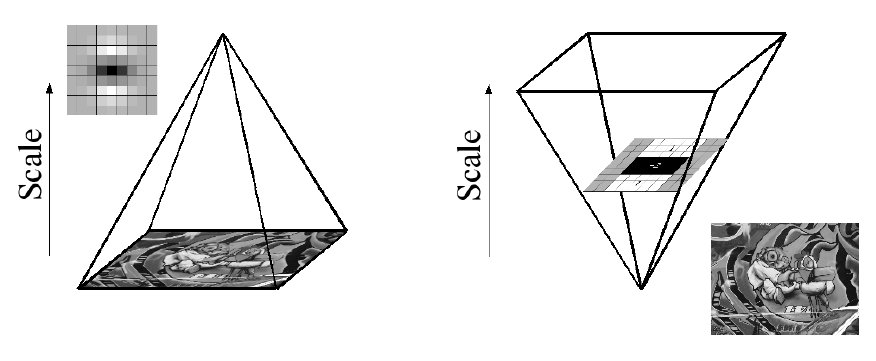
\includegraphics[scale=0.6]{./figs/pyramidfilters}
	  \caption[Pirámide de escala de imágenes para SIFT y SURF]{Pirámide de escala de imágenes para el método SIFT (izquierda) y el método SURF (derecha). (Figura tomada de \cite{Bay:2008:SRF}).}
	\label{fig:pyramidfilters}          %% Etiqueta para la figura entera
      \end{figure}

      Así el determinante de la matriz hessiana (aproximado) usado por SURF queda definido como:
\begin{equation}
      \label{eq:det_happrox}
      \det(\mathcal{H}_{approximado})=D_{xx}D_{yy}-(wD_{xy})^{2} 
      \end{equation}
con $w=0.9$ y donde $\mathit{D}_{xx}$, $\mathit{D}_{yy}$ y $\mathit{D}_{xy}$ son las derivadas parciales gaussianas de segundo orden aproximadas. La ponderación relativa $w$ de la respuesta del filtro es usada para balancear la expresión del determinante hessiano. Si bien el mismo varía para diferentes escalas, en la práctica se puede establecer este factor como constante con $w=0.9$, ya que el mismo no tiene un impacto significante en los resultados \cite{Bay:2008:SRF}.

La derivada parcial de segundo orden gaussiana en la dirección ``y'' $L_{yy}$ puede ser observada en la Fig. \ref{fig:gaussiankernelsdiscreted_y} y su homóloga aproximada $D_{yy}$ en la Fig. \ref{fig:gaussiankernelsaprox_y}; en tanto que en la Fig. \ref{fig:gaussiankernelsdiscreted_xy} se encuentra representada la derivada parcial de segundo orden gaussiana en la dirección ``x-y'' $L_{xy}$ y su homóloga aproximada $D_{xy}$ (Fig. \ref{fig:gaussiankernelsaprox_xy}).
\begin{figure}[tbhp]
	    \centering
	    %%----primera subfigura----
	    \subfloat[]{
		  \label{fig:gaussiankernelsdiscreted_y}         %% Etiqueta para la primera subfigura
		  \includegraphics[scale=0.45]{../img_ent2/gaussiankernelsdiscrete_y}}
		  \hspace{0.1\linewidth}
	    %%----segunda subfigura----
	    \subfloat[]{
		  \label{fig:gaussiankernelsaprox_y}         %% Etiqueta para la segunda subfigura
		  \includegraphics[scale=0.45]{../img_ent2/gaussiankernelsaprox_y}}
		  \hspace{0.1\linewidth}
	    %%----tercera subfigura----
	    \subfloat[]{
		  \label{fig:gaussiankernelsdiscreted_xy}         %% Etiqueta para la segunda subfigura
		  \includegraphics[scale=0.45]{../img_ent2/gaussiankernelsdiscrete_xy}}
		  \hspace{0.1\linewidth}
	    %%----cuarta subfigura----
	    \subfloat[]{
		  \label{fig:gaussiankernelsaprox_xy}         %% Etiqueta para la segunda subfigura
		  \includegraphics[scale=0.45]{../img_ent2/gaussiankernelsaprox_xy}}
		  \hspace{0.1\linewidth}
	  \caption[Derivadas parciales gaussianas discretas y aproximadas]{Derivadas parciales gaussianas de segundo orden discretas y sus homólogas aproximadas (también referenciadas como filtros tipo caja). Las regiones grises de la imagen son iguales a cero (Figuras tomadas de \cite{Bay:2008:SRF}).}%% Etiqueta para la figura entera
	    \label{fig:gaussiankernels}
      \end{figure}
      %
      Como se ha mencionado, en el método SURF se aplican sucesivamente filtros de tamaño creciente sobre la imagen original. El filtro más pequeño utilizado tiene un tamaño de $9 \times 9$ y corresponde a la derivada parcial de segundo orden de una gaussiana con $\sigma=1.2$ siendo este el nivel de escala inicial que da la máxima resolución espacial ($s=1.2$). De la misma forma, convolucionando la imagen original con filtros de mayores dimensiones se van obteniendo los niveles siguientes.

      El espacio escala para el descriptor SURF está dividido en octavas. Una octava representa una serie de respuestas obtenidas mediante la convolución de la imagen original con filtros de tamaños cada vez mayores. En total, una octava comprende un factor de escalado de 2 y cada una de ellas es subdividida en un número constante de niveles de escala (véase la Fig. \ref{fig:maximum_supression3by3by3}).
 En la Fig. \ref{fig:tamfilters1} se puede observar un esquema gráfico del análisis de 3 octavas en donde el eje horizontal, expresado logarítmicamente, representa las escalas. Notar que para cada nueva octava, el tamaño del filtro es incrementado al doble (en la primer octava el paso es 6, en la segunda de 12, en la tercera 24, etc.) y cada una de ellas empieza con un tamaño de filtro igual al segundo de la octava anterior. También, se puede observar que las octavas están solapadas, esto, con el objetivo de cubrir todas las posibles escalas. %Se hace notar para el método que cuanto más octavas son procesadas el número de puntos detectado por octavas decae rápidamente. 
 Por ejemplo, para la primer octava el espacio escala comienza con filtros de $9 \times 9$ continuando con los de $15 \times 15$, $21 \times 21$, y $27 \times 27$. Debido a que se realiza una supresión de no-máximos\footnote{La supresión de no-máximos fija en cero a todos los píxeles de una vecindad que son menores al máximo valor presente en la misma. También se utiliza el término filtro de máxima para referirse a este concepto.} tanto espacialmente como con las escalas vecinas, las respuestas del hessiano en el primer y último nivel son usadas solo para comparación. Por ello, luego de realizar una interpolación, la escala posible más pequeña es $\sigma = 1.6$ correspondiente a un filtro de $12 \times 12$, y la más grande a $\sigma = 3.2$ correspondiente a un filtro de $24 \times 24$. Consideraciones similares se aplican para las demás octavas. Para más detalles se puede consultar \cite{DBLP:phd/ch/Bay2009}.
      \begin{figure}[tbhp]
	\centering
	      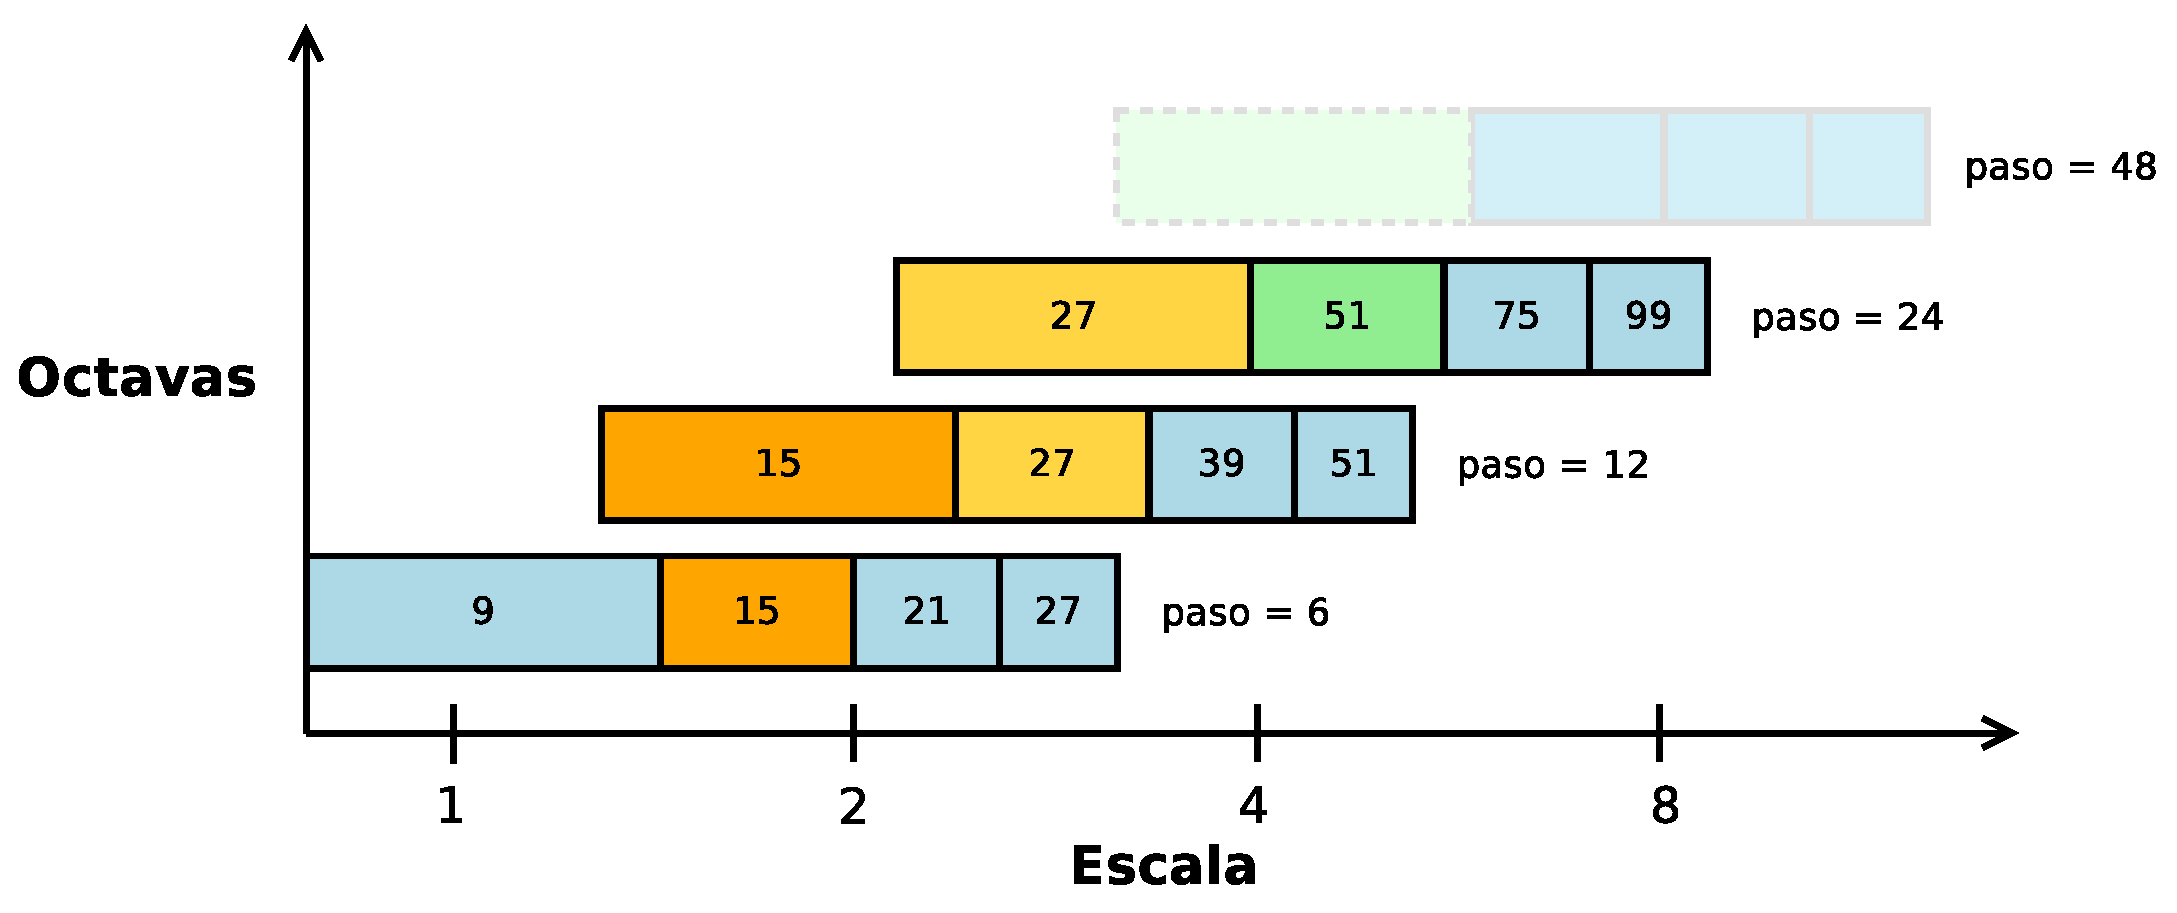
\includegraphics[scale=0.32]{./figs/tamfilters1}
	  \caption[Longitudes de los filtros para 3 diferentes octavas]{Representación gráfica de las longitudes de los filtros para 3 diferentes octavas (Figura adaptada de \cite{Bay:2008:SRF}).}
	\label{fig:tamfilters1}               %% Etiqueta para la figura entera
      \end{figure}
      \subsection{Determinación de la localización de puntos claves} %http://es.wikipedia.org/wiki/Reconocimiento_de_regiones
    Como se ha visto en la sección anterior, se construye una ``pirámide de respuestas'' con diferentes niveles de escalas dentro de las octavas. La localización de los puntos claves como su escala, se determinan hallando los extremos entre los 8 vecinos en el nivel evaluado y los $2 \times 9$ vecinos en el nivel inmediatamente superior e inferior mediante la supresión de no-máximos en la vecindad de $3 \times 3 \times 3$. Un esquema puede ser observado en la Fig. \ref{fig:maximum_supression3by3by3} donde se demarca dicha vecindad.
      \begin{figure}[tbhp]
	\centering
	      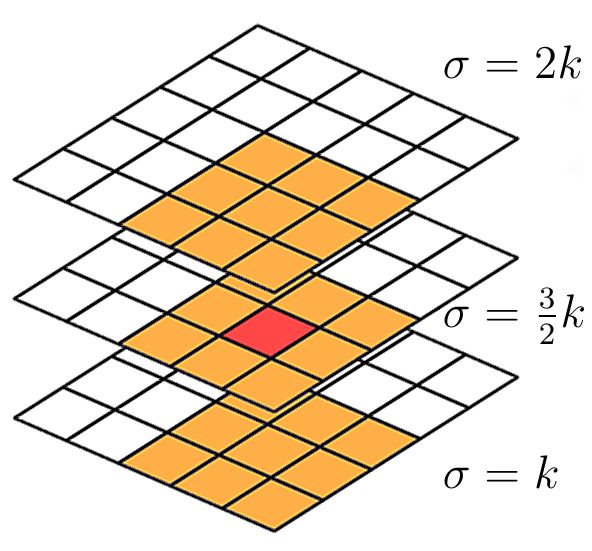
\includegraphics[scale=0.35]{./figs/333nonmaximum}
	  \caption[Representación de una octava compuesta por tres niveles de escala]{Representación de una octava compuesta por tres niveles de escala $\sigma=k$, $\sigma=\frac{3}{2}k$, $\sigma=2k$.}
	\label{fig:maximum_supression3by3by3}               %% Etiqueta para la figura entera
      \end{figure}

      	Una vez que el máximo local es identificado, la posición precisa de cada punto clave es obtenida a través de interpolación y el resultado es un conjunto de puntos claves localizados con precisión sub-píxel, los cuales están asociados a un valor de escala \cite{DBLP:phd/ch/Bay2009}.
      	
%       	Para encontrar la ubicación interpolada del punto de interés, se tienen en cuenta los máximos en la vecindad de $3 \times 3 \times 3$ en cada dimensión alrededor del máximo detectado como se ha descripto arriba. Luego se localiza el máximo mediante el ajuste de una función cuadrática 3D en el espacio escala sobre el las respuestas.
	 %De esta manera, el máximo determinante de la matriz Hessiana es interpolado en la escala y posición de la imagen. %usando 4 octavas, 8 escalas son analizadas	
% 	Cuando la búsqueda de extremos se produce en las octavas más altas, el área cubierta por los filtros resulta de un tamaño considerable y esto introduce un error significativo al momento de determinar la posición de los puntos de interés. Para solucionar este inconveniente, la determinación de la posición del punto de interés es interpolada mediante el ajuste a una función cuadrática 3D en el espacio escala mediante expansión en series de Taylor \cite{Brown02invariantfeatures}. 
% 	
% 	Así, se expresa el Hessiano como una función $H(x,y,\sigma)$ mediante la descomposición en series de Taylor \eqref{eq:expansionTaylorSeries}
% 	 para buscar los extremos estableciendo la derivada a cero y resolviendo la ecuación \eqref{eq:equationinterpolation} para encontrar $\mathbf{\hat{p}}=(x,y,s)$
% 	\begin{equation}
% 	 \label{eq:expansionTaylorSeries}
% 	 H(\mathbf{p})=H+\frac{\partial H^{\mathtt{T}}}{\partial\mathbf{p}}\mathbf{p}+\frac{1}{2}\mathbf{p}^{\mathtt{T}}\frac{\partial^{2}H^{\mathtt{T}}}{\partial\mathbf{p}^{2}}\mathbf{p}
% 	\end{equation}
% 	\begin{equation}
% 	 \label{eq:equationinterpolation}
% 	 \mathbf{\hat{p}}=\frac{\partial^{2}H^{-1}}{\partial\mathbf{p}^{2}}\,\frac{\partial H}{\partial\mathbf{p}}
% 	\end{equation}
% 	
% 	De esta forma se obtiene la ubicación de un punto de interés asociados a un valor de escala.%\cite{DBLP:phd/ch/Bay2009}
%       Una característica invariante a la escala es identificada cuando el determinante del Hessiano alcanza un máximo local en ambos espacios imagen y escala (esto es, 3x3x3 supresión de no-maximos es necesario llevar a cabo). Debemos aclarar que previamente se define un umbral mínimo para determinar cuales son los máximos que participan en la selección final.

\section{Descripción de puntos claves}
    \label{sec:descripcion_ptos_claves}
    Tras la localización y la asociación de escala a los puntos claves, la siguiente etapa consiste en asignar una orientación a cada uno de ellos para otorgarles invarianza ante la rotación mediante la orientación del mismo.
%   El descriptor SURF describe la distribución de las intensidades en una vecindad del punto clave construyendose sobre la distribución de las respuestas de las wavelets Haar de primer orden y utilizando imágenes integrales para aumentar la velocidad.
%   
%   El primer paso consiste en fijar una orientación basada en la información de una región circular alrededor del punto de interés detectado. Luego se construye una región cuadrada alineada con la orientación seleccionada y se extrae el descriptor SURF de la misma.
  \subsection{Asignación de la orientación}
    \label{sec:orientacion_del_punto}
     Para definir la orientación, primeramente se calculan las respuestas con los filtros presentados en la Fig. \ref{fig:simplekernels} sobre un área circular de radio $6s$ alrededor del punto clave, siendo $s$ la escala en que se detectó el punto. Tanto el muestreo como el tamaño de los filtros son dependientes de la escala y se establecen a $s$ y $4s$ respectivamente (a mayor escala, mayor es la dimensión de las wavelets). %(longitud del lado)
    La evaluación de los filtros realizada aquí, se vale nuevamente de las imágenes integrales para realizar los cálculos más rápidamente. Tras el cálculo de las respuestas, las mismas son ponderadas con una gaussiana de valor $\sigma=2s$ centrada en el punto clave.  
    \begin{figure}[tbhp]
       \centering
       %%----primera subfigura----
       \subfloat[]{
            \label{fig:simplekernels1}         %% Etiqueta para la primera subfigura
            \includegraphics[scale=0.4]{../img_ent2/simplekernels1harn}}
       \hspace{0.1\linewidth}
       %%----segunda subfigura----
       \subfloat[]{
            \label{fig:simplekernels2}         %% Etiqueta para la segunda subfigura
            \includegraphics[scale=0.4]{../img_ent2/simplekernels2harn}}
        \caption[Filtros Wavelets Haar]{Filtros Wavelets Haar para calcular las respuestas en la dirección $x$ \subref{fig:simplekernels1} e $y$ \subref{fig:simplekernels2}.}
       \label{fig:simplekernels}                %% Etiqueta para la figura entera
    \end{figure}
    
    Luego, las respuestas son representadas como puntos en el espacio (respuestas horizontales a lo largo del eje de abscisas $dx$ y verticales $dy$ en el de ordenadas) y la orientación dominante se determina mediante la suma de todas las respuestas en una ventana deslizante orientada de tamaño $\pi/3$, como puede observarse en la Fig. \ref{fig:responsecalculate}. Así, las respuestas horizontales y verticales dentro de la ventana son sumadas constituyendo un vector de orientación local. La orientación final para el punto clave, es aquella en la que el vector resulta ser el más largo entre todas las ventanas.
% 
%  una ventada deslizante orientada de tamaño $\frac{\pi}{3}$ detecta la orientación dominante de la respuesta de las wavelets haar ponderadas con un gaussiano en una vecindad circular alrededor del punto clave. Las dirección de respuesta horizontal y vertical están representadas por los puntos en los ejes $dx$ y $dy$ respectivamente. 
    \begin{figure}[tbhp]
      \centering
	    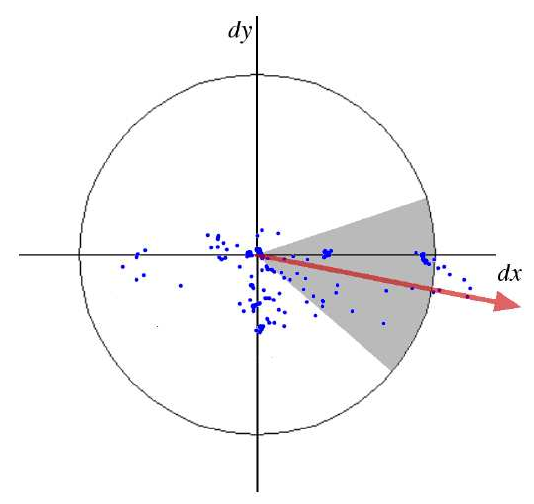
\includegraphics[scale=0.45]{./figs/responsecalculate}
	\caption[Asignación de la orientación para un punto clave]{Asignación de la orientación para un punto clave con una ventana deslizante orientada de tamaño $\frac{\pi}{3}$. (Figura tomada de \cite{Bay:2008:SRF}).}
      \label{fig:responsecalculate}                %% Etiqueta para la figura entera
    \end{figure}
   \subsection{Creación del descriptor}
      En esta última parte, se termina la creación del descriptor SURF.
      El primer paso consiste en construir una región cuadrada de tamaño $20s$ centrada en el punto de interés y orientada de acuerdo al resultado que se obtuvo en la sección \ref{sec:orientacion_del_punto}. Ejemplos de esas regiones cuadradas son ilustradas en la Fig. \ref{fig:squareregionsexample}.
      \begin{figure}[tbhp]
	\centering
	      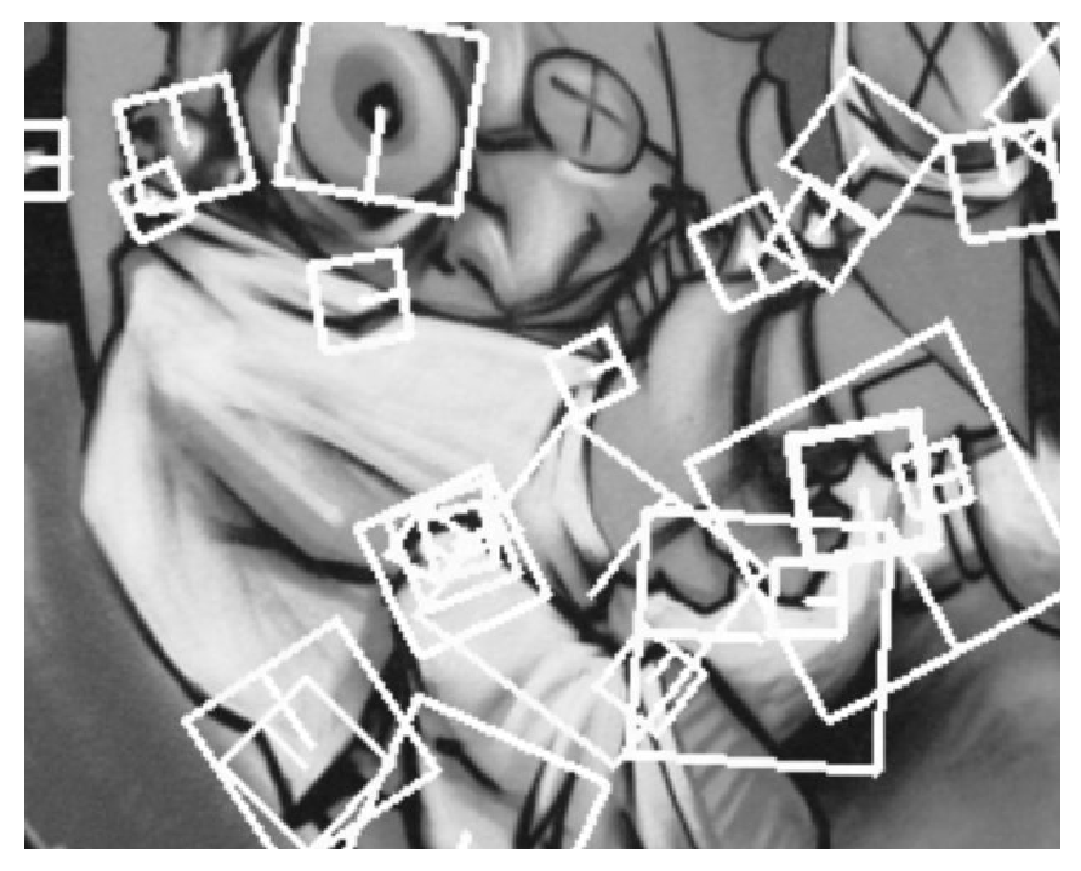
\includegraphics[scale=0.4]{./figs/squareregionsexample}
	  \caption[Ejemplo de ventanas del descriptor a diferentes escalas sobre una imagen]{Detalle de una escena mostrando el tamaño de las ventanas orientadas del descriptor a diferentes escalas. (Figura tomada de \cite{Bay:2008:SRF}).}
	\label{fig:squareregionsexample}                %% Etiqueta para la figura entera
      \end{figure}
      \begin{figure}[tbhp]
	\centering
	%%----primera subfigura----
	\subfloat[]{
	      \label{fig:subdivideregions}         %% Etiqueta para la primera subfigura
	      \includegraphics[scale=0.30]{./figs/subdivideregions}}
	\hspace{0.1\linewidth}
	%%----segunda subfigura----
	\subfloat[]{
	      \label{fig:left_boxfilters}         %% Etiqueta para la segunda subfigura
	      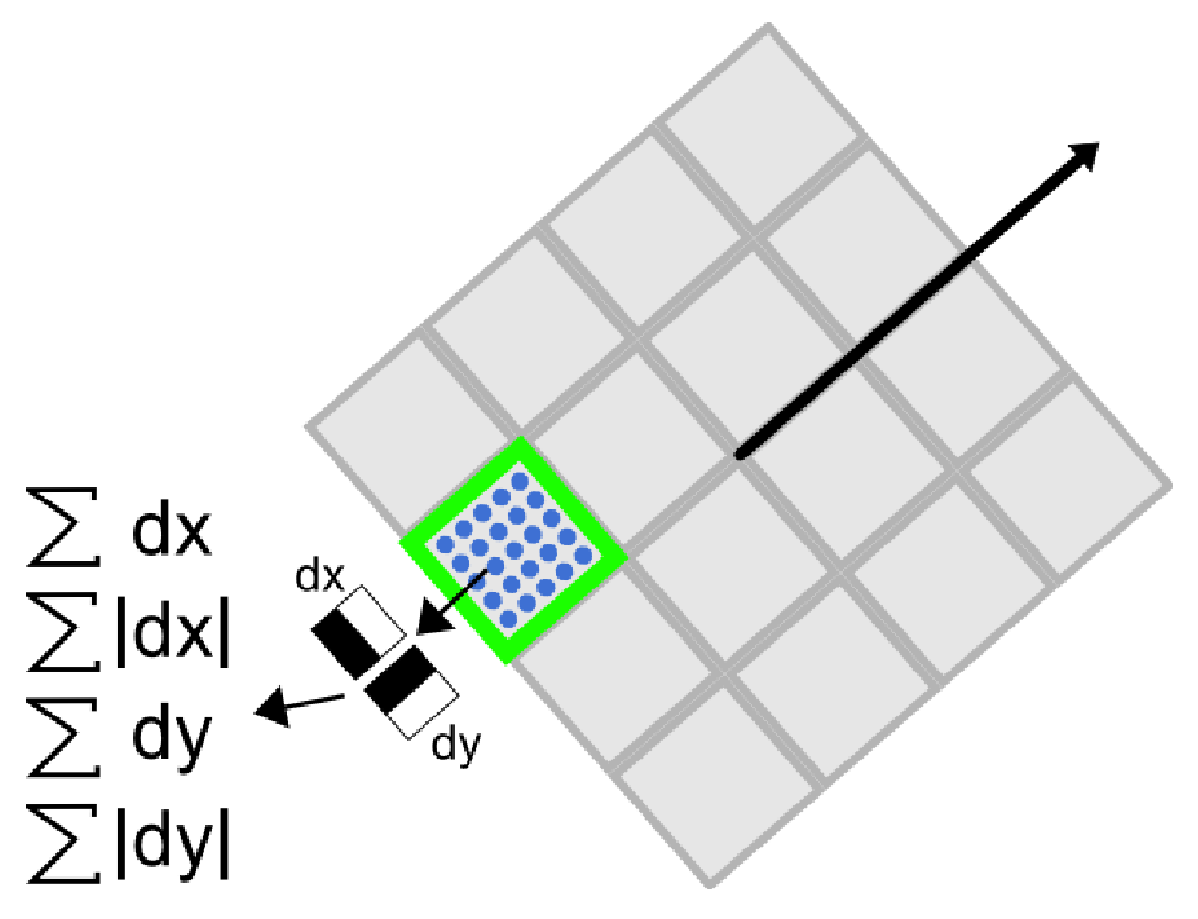
\includegraphics[scale=0.30]{./figs/respuestaswavelethaar}
	  }
	\label{fig:regioneshaarandresponses}                %% Etiqueta para la figura entera
	\caption[Interpretación gráfica del descriptor SURF]{Interpretación gráfica del descriptor SURF. (Figuras tomadas de \cite{Bay:2008:SRF}).}
      \end{figure}
      \begin{figure}[tbhp]
	\centering
	      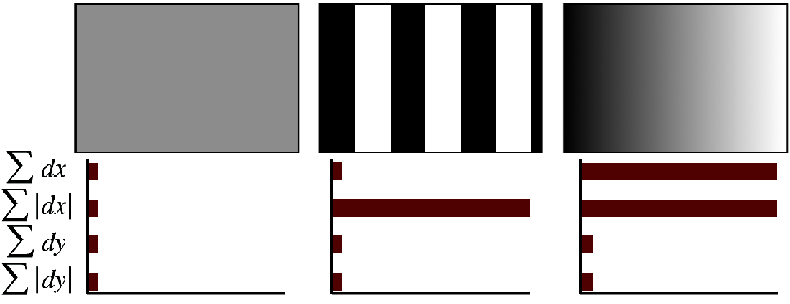
\includegraphics[scale=0.60]{./figs/descriptorresponses}
	  \caption[Descriptores resultantes para tres subregiones con patrones diferentes]{Descriptores resultantes para tres subregiones con patrones diferentes (Figura tomada de \cite{Bay:2008:SRF}).}
	\label{fig:descriptorresponses}                %% Etiqueta para la figura entera
      \end{figure}
      Seguidamente, cada región es dividida en subregiones de $4 \times 4$ como se puede observar en la grilla cuadrada orientada sobre el punto de interés en la Fig. \ref{fig:subdivideregions}. Luego para cada subregión se calculan las respuestas de las waveletes Haar con una separación de muestreo de $5 \times 5$. Las subdivisiones de $2 \times 2$ de cada cuadrado corresponden a los campos reales del descriptor que son las sumas $dx$, $|dx|$, $dy$ y $|dy|$ calculadas relativas a la orientación de la grilla como se observa en la Fig. \ref{fig:left_boxfilters} donde se denota con $d_x$ y $d_y$ a la respuesta de la wavelet Haar en la dirección horizontal y vertical respectivamente (relativas a la orientación del punto clave, con tamaño del filtro igual a $2s$). Se debe tener en cuenta que para incrementar la robustez ante deformaciones geométricas y errores de localización, las respuestas $d_x$ y $d_y$ son primero ponderadas con un gaussiano con $\sigma=3.3s$ centrado en el punto de interés. % Un ejemplo de la subdivisión y el resultado de las respuestas, puede ser observado en la Fig. \ref{fig:subdivideregions}. 
%Finalmente, el descriptor SURF consiste en las respuestas de la wavelet Haar en una región de 4x4 alrededor del punto clave \cite{Evans09noteson}.
      Luego, las respuestas $d_x$ y $d_y$ se suman en cada subregión, como así también los valores absolutos de las mismas $|dx|$ y $|dy|$ con el objetivo de brindar información de la polaridad sobre los cambios de intensidad. De esta forma, cada subregión queda representada por un vector de 4 dimensiones $\mathbf{v}$, que caracteriza su intensidad localmente $\mathbf{v}=(\sum{d_x},\sum{d_y},\sum{|d_x|},\sum{|d_y|})$. Debido a que se tienen $16$ subregiones ($4 \times 4$) con vectores de 4 dimensiones por subregión, se obtiene un vector descriptor de 64 dimensiones ($16 \times 4$) por cada punto clave detectado, por lo que se puede decir que el descriptor SURF consiste en las respuestas de la wavelet Haar en una región de 4x4 alrededor del punto clave \cite{Evans09noteson}. Las repuestas wavelet son invariantes a un sesgo en la iluminación, mientras que la invarianza al contraste es alcanzado mediante la normalización del descriptor.
 %conversión del descriptor a uno unitario.
      
      En la Fig. \ref{fig:descriptorresponses} se pueden observar los descriptores para tres subregiones con patrones de imágenes diferentes. En el caso de una región homogénea se puede observar que todos los valores son relativamente bajos; en presencia de frecuencias en la dirección de $x$, los valores de $\sum{|d_x|}$ son altos, mientras los otros son bajos y si la intensidad se incrementa gradualmente en la dirección $x$, ambos valores $\sum{d_x}$ y $\sum{|d_x|}$ son altos.
%       SURF es, hasta un cierto punto, conceptualmente similar a SIFT, en el sentido de que ambos se enfocan en la información de la distribución espacial del gradiente. Sin embargo, SURF supera a en la práctica a SIFT en todos los casos como se mostrará en la sección \ref{sec:seccion5}. Se cree que esto es debido al hecho de que SURF integra la información del gradiente en un sub parche, mientras que SIFT depende de las orientaciones de los gradientes individuales. Esto hace a SURF menos sensitivo al ruido, como se muestra en la figura \ref{fig:surflesssensitivetonoise}
      
      Si bien existen muchos parámetros del método que pueden variarse, en este capítulo se han expuestos aquellos que el autor \cite{Bay:2008:SRF} recomienda según sus resultados en la publicación original.
%%%%%%%%%%%%%%%
\section{Correspondencia entre puntos claves}
\label{sec:correspop_ptos_claves}
El término correspondencia entre puntos o entre imágenes se puede interpretar como el cálculo de un valor que represente el grado de similitud entre dos imágenes. Para ello, la correspondencia entre los puntos claves de dos imágenes es buscada mediante el cálculo de la distancia euclídea entre los vectores característicos asociados a los puntos claves detectados en cada una de las imágenes. %Este cálculo, genera un valor que es utilizado para determinar la correspondencia entre los puntos de las imágenes que se están comparando.
%Poseer un descriptor de 64 dimensiones para cada punto clave detectado, resulta útil en la medida que se tenga un método para decidir cuando un descriptor de consulta coincide con un descriptor de la imagen patrón. 
Es decir que el problema que se plantea aquí, es el de comparar los descriptores de los puntos claves de las imágenes para determinar coincidencias de puntos y así afirmar o no la presencia del objeto buscado.

El m\'etodo de búsqueda del vecino más cercano (NNS: del inglés, Nearest Neighbor Search) \cite{AryaEtAl98} es un método de gran utilidad. Se ha aplicado a gran variedad de aplicaciones como el reconocimiento de imágenes, la compresión de datos, los sistemas de recuperación de documentos, estadísticas y análisis de datos, entre otros. %Debido a que los puntos se encuentran en un espacio, estos tienen una noción de distancia (eg. la distancia euclidea).
NNS es un problema de optimización que intenta buscar los puntos más cercanos en un espacio métrico: dado un conjunto de puntos $P=\left\{ p_{1,...,}p_{n}\right\}$ en un espacio métrico $M$ y un punto de consulta $q \in M$, encontrar el punto más cercano a $q$ en $P$ de forma eficiente, donde $M$ es un espacio euclídeo d-dimensional y las distancia es medida por ejemplo mediante la distancia euclídea.

Existe una variante al algoritmo NNS denominada k-NN (k-Nearest Neighbor) que a diferencia del anterior, evalúa a qué clase pertenecen los $K$ vecinos más cercanos para decidir la clase. Así, en el caso $K=1$ se está en presencia del algoritmo NNS que se describió anteriormente

% Cada uno de los datos de entrenamiento consiste en un conjunto de vectores con sus clases asociadas con cada vector(Que rempresentaría en mi las clases)
Resolver problemas de búsqueda de vecinos más cercanos, no resulta trivial en espacios de grandes dimensiones \cite{muja_flann_2009}. No es usual encontrar algoritmos que posean un rendimiento mayor al de la búsqueda lineal (también conocida como ``búsqueda por fuerza bruta''), la cual resulta costosa computacionalmente y hasta a veces, imposible de usar en muchas aplicaciones. Es por esto, que se ha generado un gran interés en algoritmos que puedan realizar la búsqueda del vecino más cercano de forma aproximada, con lo cual es posible lograr mejoras significativas en tiempo de ejecución con errores de precisión relativamente pequeños y aceptables \cite{muja_flann_2009, Beis:1997:SIU:794189.794431}. %Para ello, se preprocesan los datos de alguna manera, de tal forma de obtener las coincidencias más rápidamente tratando de perder la menor precisión posible.

En el trabajo de Slipa-Anan y Hartley \cite{Silpa_KDTree, bb77826}, se propuso la creación de una estructura de múltiples árboles KD o K-dimensionales aleatorios conocidos por su término en inglés como \textbf{Randomized KD-Tree}, que brinda la posibilidad de obtener resultados satisfactorios en un amplio rango de problemas \cite{muja_flann_2009}. Más específicamente, para casos en los que se trata con vectores similares a los presentados en la Sec. \ref{sec:descripcion_ptos_claves} resulta una alternativa aceptable. Por ello, se utilizará el método descripto en \cite{Silpa_KDTree, bb77826} con los parámetros estudiados que se describen en \cite{muja_flann_2009}.
\subsection{El algoritmo de árboles KD aleatorio}
El algoritmo KD-tree clásico resulta eficiente con datos de bajas dimensiones \cite{Friedman:1977:AFB:355744.355745}, pero su rendimiento se ve afectado rápidamente al aumentar la dimensionalidad de los datos. 
Para obtener una velocidad mayor a la de la búsqueda lineal, se hace necesario establecer una búsqueda aproximada del vecino más cercano. Esto mejora el tiempo de búsqueda pero, como contrapartida, el algoritmo no siempre da como resultado el vecino más cercano. Para realizar esta búsqueda aproximada de forma rápida, se crea una estructura de árbol que contribuye a la reducción en los tiempos de procesamiento.% Un árbol KD es una estructura de datos jerárquica construida mediante el particionamiento recursivo de los datos a lo largo de la dimensión de mayor varianza usada para resolver rápidamente problemas del vecino más cercano.

Los elementos guardados en el árbol KD-tree, son vectores de altas dimensiones. En la raíz del árbol (primer nivel), los datos son divididos en dos mitades por un hiper plano ortogonal para una dimensión elegida y con un valor de umbral. Generalmente, esta división se realiza con la media, en la dimensión con la mayor varianza del conjunto de datos. En características visuales provistas por SIFT o SURF, utilizar la media en la dimensión con mayor varianza es la que presenta el mejor rendimiento \cite{muja_flann_2009}. Para construir el árbol, se compara el vector de entrada con el ``valor de partición'' para determinar a qué mitad del árbol pertenece dicho vector.
Cada una de las dos mitades de los datos es dividida de igual manera y en forma recursiva, para lograr crear un árbol binario completamente balanceado.
% Cada nodo de la parte inferior del \'arbol corresponde a un punto simple del conjunto de datos. 
% Sin embargo, en algunas aplicaciones los nodos hojas pueden tener más de un punto.
%Slipa-Anan y Hartley \cite{Silpa_KDTree}, han propuesto una versión del algoritmo de árbol KD en el que múltiples árboles KD aleatorios son creados \cite{Silpa_KDTree, bb77826}. 
% Como se ha mencionado, el algoritmo de árboles KD original, divide los datos en mitades %por la mitad 
% en cada nivel del árbol, en la dimensión para la cual los datos exhiben la mayor varianza.

A diferencia del algoritmo KD-tree clásico, los árboles aleatorios son construidos seleccionando la dimensión de división de forma aleatoria sobre las primeras $D$ dimensiones en las que los datos poseen mayor varianza. 
Se usa el valor fijo $D=5$ que resulta el más adecuado para diferentes datos \cite{muja_flann_2009}. %Un ajuste adicional sobre dicho valor, no otorga beneficios importantes.
%en vez de usar x, y, x y para decidir para que lado tira el nodo, saca la varianza en el nivel, selecciona las 5 más variantes y sobre esas aleatoriamente toma una.

Cuando se realiza la b\'usqueda en el árbol, una cola con prioridad es mantenida a través de todos los árboles aleatorios, por lo que la búsqueda queda ordenada mediante el incremento de la distancia a cada nodo del borde. 
El grado de aproximación, se determina mediante el examen de un número fijo de nodos hoja. Cuando es alcanzado este número, se termina la búsqueda y se obtienen los candidatos. 
Se debe tener en cuenta que la cantidad de memoria utilizada aumenta linealmente con el número de árboles aleatorios, una característica negativa cuya importancia no resulta menor en la sobrecarga del sistema.

\subsection{Remoción de correspondencias no válidas}
\label{sec:remocion_corresp_invalidas}
La utilización de la forma de búsqueda de coincidencias descripta en la sección anterior no resulta del todo adecuada, ya que para un punto clave de consulta siempre se encontrarán valores de correspondencias que no necesariamente son válidos. Por ello, se hace necesario la aplicación de un umbral para determinar las potenciales correspondencias válidas. Usar un valor de umbral global que se compare con la distancia a la característica más cercana no funciona correctamente
%, ya que algunos descriptores son más discriminativos que otros 
según lo afirma Lowe \cite{Lowe:2004:DIF:993451.996342}. Por ello, se propone considerar una medida más efectiva obtenida mediante la comparación de la distancia del vecino más cercano respecto del segundo vecino más cercano. Así la estrategia que se propone en \cite{Lowe:2004:DIF:993451.996342} es la utilizada en este trabajo y es la que se describe a continuación.

Sean $A$ y $B$ dos imágenes sobre las cuales se quieren buscar correspondencias. Consideremos $a_i$ con $i=0\ldots n$ un punto del conjunto de puntos claves detectados en $A$, $n$ el total de puntos claves detectados en $A$, $av_i$ el vector característico asociado al punto $a_i$ y de forma similar para la imagen $B$. Para cada $a_i$, se seleccionan los dos mejores puntos claves candidatos $p_1 \in b_i$ y $p_2 \in b_i$ cuyos vectores de características asociados a cada uno representan las distancias euclídeas mínimas $d_1$ y $d_2$ respectivamente respecto a $av_i$. Luego, si se cumple la proporción $\frac{d_{1}}{d_{2}}>\varepsilon\qquad(\varepsilon=0.8\:\cite{Lowe:2004:DIF:993451.996342})$ la coincidencia es rechazada.
El valor de $\varepsilon=0.8$ fue seleccionado de acuerdo al estudio llevado a cabo por Lowe \cite{Lowe:2004:DIF:993451.996342} que afirma que se alcanzan a eliminar un 90\% de falsas coincidencias mientras se descartan sólo un 5\% de buenas coincidencias, resultando en el valor más apropiado. %Valores de $\varepsilon=0.6$ a $0.9$ también son apropiados.

Esta remoción de pares de correspondencias, que resultan presuntamente pares inadecuados, reduce el número de pares disponibles para buscar la correspondencia pero realza la habilidad de buscar la homografía correcta mediante la reducción de correspondencias incorrectas.
% En muchos casos el objeto plano buscado contiene muchas características genericas como esquinas o simples curvas. Este problema ocurre comunmente cuando se buscan simple logos. Estas características pueden ser encontradas muchas veces en la imagen objetivo y pueden producir que no se encuentre la homografía correcta. Esta remoción reduce el numero de pares dispnibles para buscar la correspondencia, pero realza la habilidad de buscar la homografía correcta mediante la reducción de correspondencias incorrectas.
\section[Formación de la imagen y transformación proyectiva]{Conceptos de formación de la imagen y transformación proyectiva}
Hasta el momento, se ha descripto la forma de obtener puntos claves y vectores descriptores sobre imágenes y mediante la correspondencia de características, determinar la similitud entre dos imágenes. Sin embargo, aún no se tiene suficiente información para determinar la posición del objeto buscado. Para ello, es necesario introducir algunos conceptos básicos de formación de la imagen que se explicarán a continuación.
% Para ello, se tratarán diversos temas entre los que podemos mencionar: el proceso de formación de la imagen y el modelo de cámara oscura, la calibración de la cámara y los parámetros extrínsecos e intrínsecos de la misma, 
\subsection{Introducción}
El principal componente para la visión en una escena es la luz. La misma proviene como un rayo que sale de una fuente (por ejemplo: el sol o una lámpara) y viaja a través del espacio hasta intersectar un objeto donde parte de la luz es absorbida y otra reflejada (percibida como el color) la cual es captada por los ojos (o cámara) y recogida en la retina (o imagen).
% La geometría de esta estructura, es de particular importancia práctica en visión computacional.

Existen diversos dispositivos para obtener imágenes, uno de los más comunes, es la cámara digital. Ésta captura la escena mediante la proyección de luz en un sensor a través del lente de la cámara. El hecho de que la imagen se forma a través de la proyección de la escena 3D en un plano 2D, implica la existencia de importantes relaciones entre la escena y su imagen, y es la geometría proyectiva la herramienta usada para describir y caracterizar en términos matemáticos este proceso de formación de la imagen \cite{citeulike:3484001, citeulike:9456628}.
%%%%%%%%%%%%%%%%%%%%%%%%%%%%%%%%%%%%%%%%%%%%%%%%%%%%%%%%%%%%%%%%%%%%%%%%%%%%%%%%%%%%%%%%%%%%%%%
%%%%%%%%%%%%%%%%%%%%%%%%%%%%%%%%%%%%%%%%%%%%%%%%%%%%%%%%%%%%%%%%%%%%%%%%%%%%%%%%%%%%%%%%%%%%%%
%%%%%%%%%%%%%%%%%%%%%%%%%%%%%%%%%%%%%%%%%%%%%%%%%%%%%%%%%%%%%%%%%%%%%%%%%%%%%%%%%%%%%%%%%%%%%%
%%%%%%%%%%%%%%%%%%%%%%%%%%%%%%%%%%%%%%%%%%%%%%%%%%%%%%%%%%%%%%%%%%%%%%%%%%%%%%%%%%%%%%%%%%%%%%
Existe un modelo teórico útil denominado \textbf{modelo de cámara oscura} (del inglés: \textbf{``pinhole camera model''}) \cite{Hartley2004, citeulike:3484001} con el cual se puede entender la geometría básica en la proyección de rayos. %\ref{subsubsection_formacion_imagen}. %Sin embargo, un modelo de este tipo no puede ser aplicado realmente para obtener imágenes en la vida real, ya que el mismo no puede recoger la suficiente cantidad de luz en una exposición rápida. Es por esto que las cámaras usan lentes (los cuales introducen distorsiones no deseables) para obtener más luz de la disponible para un punto dado.
% % Un ``pinhole''  un orificio de apertura pequeña en el centro de una pared imaginaria. 
% %Estas desviaciones provocadas por la lente, pueden ser corregidas matemáticamente a través de la calibración de la cámara, técnica mediante la cual se puede obtener tanto el modelo geométrico de la cámara como el modelo de distorsión de la lente, los cuales pasan a formar parte de los parámetros  de la cámara y son denominados intrínsecos.
% 
% \subsection{Formación de la imagen}
% \label{subsubsection_formacion_imagen}
% El proceso de formación de la imagen no ha cambiado desde los comienzos de la fotografía \cite{citeulike:9456628}. La luz proveniente de la escena observada, es capturada por la cámara a través de la apertura frontal y los rayos de luz impactan en el plano de la imagen (o sensor de imagen) localizado por detrás de la cámara, en donde un lente es usado para concentrar los rayos provenientes de los diferentes elementos de la escena. Este proceso, se ilustra en la Fig. \ref{fig:figura_image_formation_1}, donde $do$ es la distancia de la lente al objeto observado, $di$ es la distancia de la lente al plano de la imagen y $f$ es denominada \textbf{distancia focal}. Estas variables, se encuentran relacionadas mediante la ecuación de la lente \eqref{eq:eq_ecuacion_lente}.
% 
% \begin{figure}[tbhp]
% \centerline{\includegraphics[scale=0.5]{../entregable04/img/imgformation1}}
% \caption[Formación de la imagen]{Formación de la imagen. Adaptada de \cite{citeulike:9456628}. }
% \label{fig:figura_image_formation_1}
% \end{figure}
% 
% \begin{equation}
%  \frac{1}{f}=\frac{1}{do}+\frac{1}{di}
% \label{eq:eq_ecuacion_lente}
% \end{equation}
% 
% En visión computacional, este modelo de cámara puede ser simplificado mediante ciertas consideraciones:
% \begin{itemize}
%  \item Se asume nulo el efecto de la lente (distorsión),
%  \item Se considera una cámara con una apertura infinitesimal: de esta forma sólo se considera el rayo central,
%  \item Se asume $do>>di$: esto significa que el plano de la imagen está en la posición de la distancia focal (enfocado),
%  \item De la geometría del sistema, puede observarse que el objeto resulta invertido en el plano de la imagen: se puede obtener una imagen idéntica, pero no invertida simplemente posicionando el plano de la imagen en frente de la lente (aunque esto no es físicamente posible, es completamente equivalente desde un punto de vista matemático).
% \end{itemize}
% Este modelo simplificado, es conocido como ``modelo de cámara oscura'' y se representa en la Fig. \ref{fig:figura_image_formation_2}
% \begin{figure}[tbhp]
% \centerline{\includegraphics[scale=0.5]{../entregable04/img/imgformation2}}
% \caption[Modelo pin\-hole de la cámara]{Modelo pin\-hole de la cámara. Adaptada de \cite{citeulike:9456628}.}
% \label{fig:figura_image_formation_2}
% \end{figure}
% 
% Usando la ley de similitud de triángulos y observando el modelo mencionado, se puede derivar la ecuación de proyección \eqref{eq:eq_ecuacion_proy} de la cual se desprende que: el tamaño $hi$ de un objeto de altura $ho$ en el plano imagen, resulta inversamente proporcional a la distancia $do$ entre la cámara y el objeto. Esta relación, es fácilmente observable: cuando se fotografía un objeto cercano a la cámara, el mismo  aparece de mayor tamaño en el plano de la imagen; por el contrario si el objeto es alejado de la misma, éste aparece de menores dimensiones en el plano de la imagen. De esta manera se puede obtener la posición de un punto 3D de la escena, en el plano imagen.
% 
% \begin{equation}
%  hi=f\frac{ho}{do}
% \label{eq:eq_ecuacion_proy}
% \end{equation}
% 
% \subsection{Calibración de la cámara}
% De la sección \ref{subsubsection_formacion_imagen}, se vio que los parámetros esenciales de la cámara son la distancia focal y el tamaño del plano de la imagen.
% % (que define el campo de vista de la cámara). 
% Cuando se trata de imágenes digitales, la cantidad de píxeles en el plano de la imagen resulta ser otro parámetro importante a determinar con el objetivo de calcular la posición %en coordenadas 
% de un punto de la escena en el plano de la imagen. Si consideramos la línea ortogonal al plano de la imagen proveniente del punto focal, necesitamos saber en que píxel esta línea perfora el plano de la imagen. Este punto es llamado \textbf{``punto principal''}. Si bien resulta lógico asumir que este punto está en el centro del plano de la imagen, esto sólo se puede aseverar en condiciones ideales, ya que en la práctica el mismo se encuentra desplazado dependiendo de la precisión de fabricación de la cámara. Es por ello, que se necesita un proceso de calibración de la misma.
% 
% La calibración de la cámara es el proceso, por el cual son obtenidos diferentes parámetros tales como la matriz de ésta y los parámetros de distorsión (ignorados en el modelo de cámara oscura mencionado anteriormente) \cite{citeulike:3484001, citeulike:9456628}. %Uno puede obviamente usar las especificaciones provistas por el fabricante, pero para algunas tareas, como ser la reconstrucción 3D, estas especificaciones no son lo suficientemente precisas.
% % Existen técnicas para lograr calibrar la cámara cuya salida son la matriz de la cámara y los parámetros de distorsión (anteriormente en el modelo pin-hole de la cámara hemos obviado los efectos de la lente, pero esto es posible solamente cuando el lente usado en la captura de las imágenes no introduce distorsiones ópticas importantes. 
% % Para poder corregir estas distorsiones, existen diversas ecuaciones matemáticas que dan como resultado una imagen sin distorsiones visibles).
% 
% Para explicar los resultados de la calibración de la cámara, debemos referirnos a lo descripto en el modelo de cámara oscura introducido en la sección \ref{subsubsection_formacion_imagen}, para así entender la relación entre un punto 3D de la escena $P$ en la posición $(X,Y,Z)$ y su correspondiente en el plano de la imagen $p$ en la posición $(x,y)$, especificado en coordenadas de píxeles.
% 
% \begin{figure}[tbhp]
% \centerline{\includegraphics[scale=0.5]{../entregable04/img/imgformation3}}
% \caption[Calibración de la cámara]{Calibración de la cámara. Adaptada de \cite{citeulike:9456628}.}
% \label{fig:figura_image_formation_3}
% \end{figure}
% 
% En la figura \ref{fig:figura_image_formation_3}, se ha re dibujado el modelo de cámara oscura, en el que se ha agregado un cuadro de referencia posicionado en el centro de proyección. De esta figura y del análisis geométrico anteriormente mencionado, se puede derivar que el punto $P(X,Y,Z)$ será proyectado en el plano de la imagen en $(fX/Z, fY/Z)$. Si queremos trasladar éstas coordenadas a píxeles, necesitamos dividir la posición 2D de la imagen por el ancho del píxel $px$ y su altura $py$ respectivamente. Dividiendo la distancia focal $f$ (en coordenadas del mundo real) por $px$, obtenemos la distancia focal expresada en píxeles $fx$ horizontales; similarmente $fy=f/py$ es definida como la distancia focal expresada en unidades de píxeles verticales. De esta forma, la ecuación proyectiva resulta como en \eqref{eq:equation_proyectiva}, donde $(u_0, v_0)$ es el punto principal que es sumado al resultado con el objetivo de mover el origen a la esquina superior izquierda de la imagen. Éstas ecuaciones, pueden ser reescritas en forma de matriz a través de la introducción de coordenadas homogéneas, en el que un punto 2D es representado por un vector en $R^3$ y un punto 3D por uno en $R^4$, en donde la componente extra es un factor de escala arbitrario. % que debe ser eliminado cuando una coordenada 2D necesita ser extraída de un vector homogéneo de $R^3$.
% \begin{eqnarray}
% \label{eq:equation_proyectiva}
%  x=\frac{f_x X}{Z}+u_0 \nonumber \\
%  y=\frac{f_y Y}{Z}+v_0
% \end{eqnarray}
% 
% La ecuación proyectiva reescrita se puede observar en \eqref{eq:eq_ecuacion_proy_homogeneous_coordinates}.
% \begin{equation}
%   s\begin{bmatrix}x\\
%   y\\
%   1
%   \end{bmatrix}=\begin{bmatrix}f_{x} & 0 & u_{0}\\
%   0 & f_{y} & v_{0}\\
%   0 & 0 & 1
%   \end{bmatrix}\begin{bmatrix}1 & 0 & 0 & 0\\
%   0 & 1 & 0 & 0\\
%   0 & 0 & 1 & 0
%   \end{bmatrix}\begin{bmatrix}X\\
%   Y\\
%   Z\\
%   1
%   \end{bmatrix}
%   \label{eq:eq_ecuacion_proy_homogeneous_coordinates}
% \end{equation}
% 
% Los \textbf{parámetros intrínsecos} de la cámara se encuentra representados en la primer matriz de la expresión \eqref{eq:eq_ecuacion_proy_homogeneous_coordinates} y resultan constantes para un sistema lente-camara mientras que la segunda matriz es denominada matriz de proyección. Cuando el cuadro de referencia, no está en el centro de proyección de la cámara, necesitamos agregar una matriz de rotación $R$ de 3x3 y un vector de traslación $t$ de 3x1. Estas dos matrices describen las transformaciones rígidas que deben ser aplicadas a un punto 3D con el objetivo de llevarlo al marco de referencia de la cámara. Luego, se puede reescribir la ecuación de proyección de forma más general como en \eqref{eq:eq_ecuacion_proy_homogeneous_coordinates_general}
% \begin{equation}
%   s\begin{bmatrix}x\\
%   y\\
%   1
%   \end{bmatrix}=\begin{bmatrix}f_{x} & 0 & u_{0}\\
%   0 & f_{y} & v_{0}\\
%   0 & 0 & 1
%   \end{bmatrix}\begin{bmatrix}r_1 & r_2 & r_3 & t_1\\
%   r_4 & r_5 & r_6 & t_2\\
%   r_7 & r_8 & r_9 & t_3
%   \end{bmatrix}\begin{bmatrix}X\\
%   Y\\
%   Z\\
%   1
%   \end{bmatrix}
%   \label{eq:eq_ecuacion_proy_homogeneous_coordinates_general}
% \end{equation}
% 
% Las componentes de rotación y traslación, son llamados \textbf{parámetros extrínsecos} de la calibración y resultan ser diferentes para cada punto de vista.
%%%%%%%%%%%%%%%%%%%%%%%%%%%%%%%%%%%%%%%%%%%%%%%%%%%%%%%%%%%%%%%%%%%%%%%%%%%%%%%%%%%%%%%%%%%%%%
%%%%%%%%%%%%%%%%%%%%%%%%%%%%%%%%%%%%%%%%%%%%%%%%%%%%%%%%%%%%%%%%%%%%%%%%%%%%%%%%%%%%%%%%%%%%%%
%%%%%%%%%%%%%%%%%%%%%%%%%%%%%%%%%%%%%%%%%%%%%%%%%%%%%%%%%%%%%%%%%%%%%%%%%%%%%%%%%%%%%%%%%%%%%%
%%%%%%%%%%%%%%%%%%%%%%%%%%%%%%%%%%%%%%%%%%%%%%%%%%%%%%%%%%%%%%%%%%%%%%%%%%%%%%%%%%%%%%%%%%%%%%
% \subsection{Matriz fundamental de un par de imágenes}
% \label{subsub_calculo_matriz_fundamental}
% Al tomar dos imágenes de una misma escena desde diferentes puntos de vista, existe una importante relación proyectiva entre estas y la escena. Estas imágenes, pueden haber sido obtenidas mediante la misma cámara (tomando la fotografía desde dos puntos de vistas diferentes), o mediante dos cámaras posicionadas en diferentes lugares observando el mismo punto.% Cuando las cámaras están separadas por una linea de base rígida, se usa el término de visión estéreo.
% 
% Si consideramos dos cámaras observando el mismo punto $X$ en una escena, como se puede ver en la Fig. \ref{fig:figura_image_formation_4_plano_completo}, hemos visto que podemos encontrar la proyección del punto en los planos de las imágenes $x$ y $x'$ correspondiente a la posición de la cámara en $O$ y $O'$ respectivamente, trazando una línea de unión entre $X$ y el centro de la cámara. 
% 
% \begin{figure}[tbhp]
% \centerline{\includegraphics[scale=0.5]{../entregable04/img/imgformation4planocompleto}}
% \caption[Geometría epipolar]{Geometría epipolar: $O$ y $O'$ corresponden a la posición de la cámara en un instante; $X$ representa un punto de la escena a fotografiar y $p$ y $p'$ son el plano imagen obtenido de la proyección del punto $X$ con la cámara en la posición $O$ y $O'$ respectivamente. Adaptada de \cite{citeulike:9456628}.}
% \label{fig:figura_image_formation_4_plano_completo}
% \end{figure}
% 
% Ahora, si conocemos la proyección del punto $X$ sobre el plano $p$, pero desconocemos la ubicación de $X$ y su proyección correspondiente sobre el plano $p'$ como se muestra en la Fig. \ref{fig:imgformation4fulldetallesxdesconocido}, el punto $X$ puede ser localizado en cualquier lugar de la línea de unión entre $O$ y $x$. Esto, implica que si queremos buscar la correspondencia de un punto de una imagen dada $p$ en otra $p'$, debemos buscar a lo largo de la linea de proyección $l'$ en el plano de la segunda imagen. Esta línea imaginaria $l'$ recibe el nombre de \textbf{línea epipolar} del punto $x$. 
% 
% \begin{figure}[tbhp]
% \centerline{\includegraphics[scale=0.5]{../entregable04/img/imgformation4fulldetallesxdesconocido}}
% \caption[Línea epipolar]{Línea epipolar: Se desconoce la posición del punto $X$ en la escena. Se conoce la proyección de punto $X$ sobre el plano $p$ pero no sobre $p'$. Adaptada de \cite{citeulike:9456628}.}
% \label{fig:imgformation4fulldetallesxdesconocido}
% \end{figure}
% 
% El párrafo anterior, define una restricción fundamental que deben cumplir los puntos correspondientes: la correspondencia de un punto dado en una vista, debe estar en la línea epipolar del punto en la otra vista, en donde la orientación exacta de la línea epipolar viene dada por la posición respectiva de las dos cámaras, de esta forma se puede aseverar que la posición de las líneas epipolares, caracterizan la geometría de un sistema con dos puntos de vistas. Además, todas las líneas epipolares pasan a través del mismo punto el cual recibe el nombre de \textbf{epipolo}.
% 
% Matemáticamente, se puede demostrar \cite{citeulike:9456628} que la relación entre un punto de una imagen y su correspondiente línea epipolar, puede ser expresada usando una matriz $F$ de 3x3 como la \eqref{eq:eq_ecuacion_rel_pto_epipolar}. En geometría proyectiva, una línea 2D viene representada por un vector en $R^3$ que corresponde al conjunto de puntos 2D $(x',y')$ que satisfacen la ecuación $l_1'x'+l_2'y'+l_3'=0$, donde la prima denota que la línea pertenece a la segunda imagen. Consecuentemente, la \textbf{matriz fundamental} $F$, mapea un punto de una imagen 2D de una vista, a una línea epipolar en la otra vista; es decir que esta matriz proporciona para un punto en una imagen, la ecuación de la línea en la que su punto correspondiente (en la otra vista) puede ser hallado.
% Finalmente, para estimar la matriz fundamental de un par de imágenes se procede mediante la resolución de un sistema de ecuaciones.
% % Cabe aclarar que es necesario contar con un mínimo de siete correspondencias de puntos entre las imágenes.
% 
% \begin{equation}
%   \begin{bmatrix} l_1' \\
%   l_2'\\
%   l_3'
%   \end{bmatrix}=F
%   \begin{bmatrix}
%   X\\
%   Y\\
%   1
%   \end{bmatrix}
%   \label{eq:eq_ecuacion_rel_pto_epipolar}
% \end{equation}
% 
% Sea $q$ un punto expresado en coordenadas homogéneas, $q'$ el punto correspondiente a $q$ y $F$ la matriz fundamental entre las dos vistas; dado que $q'$ se encuentra en la línea epipolar $Fq$, la ecuación \eqref{eq:eq_ecuacion_rel_between_two_corresponding_points} recibe el nombre de \textbf{restricción epipolar}. Esta ecuación pone en relevancia la relación existente entre dos puntos correspondientes y es mediante la misma que se puede calcular las entradas de la matriz. Dado que las entradas de la matriz $F$ se encuentran afectadas por un factor de escala, sólo hay ocho entradas a estimar (la novena puede ser arbitrariamente establecida a 1). Cada correspondencia se refleja en una ecuación, luego, con ocho correspondencias conocidas la matriz puede ser estimada resolviendo el conjunto de ecuaciones lineales. Pero aún se puede adicionar una restricción más: matemáticamente la matriz $F$ mapea un punto 2D en una línea 1D (es decir líneas que se intersectan en un punto en común). El hecho de que estas líneas epipolares pasan a través de un único punto (el epipolo) impone una restricción a dicha matriz, reduciendo así el número de correspondencias requeridas para realizar la estimación a siete ecuaciones y por lo tanto, siete correspondencias.
% \begin{equation}
%   q'^tFq=0
%   \label{eq:eq_ecuacion_rel_between_two_corresponding_points}
% \end{equation}
% 
% Debemos mencionar que la selección de un conjunto de correspondencias apropiadas de la imagen, resulta ser de vital importancia para obtener una estimación precisa de la matriz fundamental. En general, las correspondencias deberían estar bien distribuidas a través de las imágenes y deberían incluir puntos a diferentes profundidades de la escena, en caso contrario, la solución no será la esperada resultando en valores espurios.
\subsection{El modelo de cámara oscura}
La cámara oscura es un instrumento óptico, que permite obtener una proyección plana de una imagen externa en la pared interna de una caja. La simplificación presentada en el modelo de cámara oscura es el fundamento del funcionamiento de las cámaras fotográficas. A continuación, se presentan diferentes pasos a través de los cuales se generalizará progresivamente el modelo básico de cámara oscura para entender la geometría básica en la proyección de rayos.

Consideremos la proyección central de puntos en el espacio sobre un plano. Sea $\mathbf{C}$ el centro de proyección (\textit{centro de la cámara} o \textit{centro óptico}) como origen de un sistema de coordenadas euclídeo, $\mathsf{Z}=f$ el \textit{plano de la imagen} o \textit{plano focal}, $p$ el \textit{punto principal} y considerando que el plano de la imagen está posicionado enfrente del centro de la cámara. Bajo el modelo de cámara oscura, el punto $\mathbf{X}=(\mathsf{X},\mathsf{Y},\mathsf{Z})^\mathsf{T}$ en el espacio, es mapeado a un punto en el plano de la imagen dado por la intersección del mismo, con la línea que une $\mathbf{X}$ con el centro de proyección $C$ como se puede observar en la Fig. \ref{fig:pinholemodel}. Mediante el análisis geométrico de la Fig. \ref{fig:pinholemodel_geometria}, se puede calcular que el punto $\mathbf{X}$ de la escena es mapeado al plano de la imagen en el punto $\mathbf{x}=(\mathit{f}\mathsf{X}/\mathsf{Z}, \mathit{f}\mathsf{Y}/\mathsf{Z}, f)^\mathsf{T}$. Ignorando la última componente, el mapeo del sistema de coordenadas global al de coordenadas de la imagen (un mapeo de un espacio Euclídeo $\mathbb{R}^3$ a uno en $\mathbb{R}^2$) puede expresarse mediante la notación \eqref{eq:mapeo}, asumiéndose que el origen de coordenadas en el plano de la imagen se encuentra en el punto principal.
\begin{equation}
  \label{eq:mapeo}
  (\mathsf{X},\mathsf{Y},\mathsf{Z}) \mapsto (\mathit{f}\mathsf{X}/\mathsf{Z}, \mathit{f}\mathsf{Y}/\mathsf{Z})^\mathsf{T}.
\end{equation}
\begin{figure}[tbhp]
	\centering
	%%----primera subfigura----
	\subfloat[]{
	      \label{fig:pinholemodel}         %% Etiqueta para la primera subfigura
	      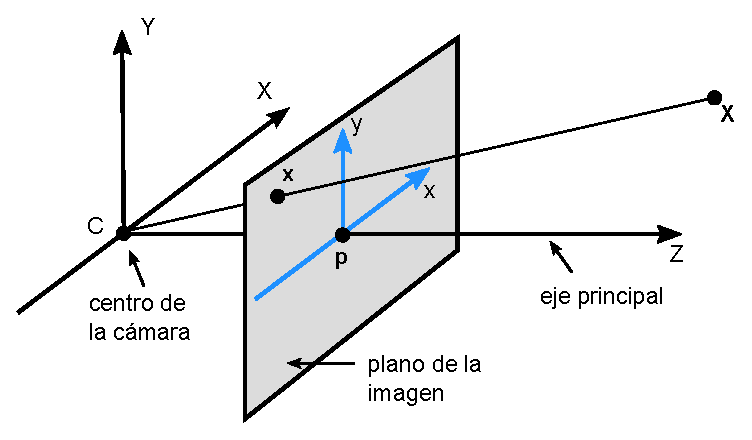
\includegraphics[scale=0.6]{../figs/sizzerman/pinholemodel}}
	\hspace{0.1\linewidth}
	%%----segunda subfigura----
	\subfloat[]{
	      \label{fig:pinholemodel_geometria}         %% Etiqueta para la segunda subfigura
	      \includegraphics[scale=0.6]{../figs/sizzerman/pinholemodelgeometria}
	  }
	\label{fig:pinholecmaeramodelinterpretation}                %% Etiqueta para la figura entera
	\caption[Modelo de cámara oscura y su interpretación geométrica]{Modelo de cámara oscura \subref{fig:pinholemodel} y su interpretación geométrica \subref{fig:pinholemodel_geometria}. (Figuras adaptadas de \cite{Hartley2004}).}
\end{figure}

Si los puntos son representados mediante una representación homogénea, la proyección central puede expresarse como un mapeo lineal entre coordenadas homogéneas y la notación \eqref{eq:mapeo} puede re-expresarse como en la ecuación \eqref{eq:eq_mapeo_matricial}.
\begin{equation}
\label{eq:eq_mapeo_matricial}
\left(\begin{array}{c}
\mathsf{X}\\
\mathsf{Y}\\
\mathsf{Z}\\
1
\end{array}\right)\mapsto\left(\begin{array}{c}
f\, \mathsf{X}\\
f\, \mathsf{Y}\\
\mathsf{Z}
\end{array}\right)=\left[\begin{array}{cccc}
f & \quad & \quad & 0\\
\quad & f & \quad & 0\\
\quad & \quad & 1 & 0
\end{array}\right]\left(\begin{array}{c}
\mathsf{X}\\
\mathsf{Y}\\
\mathsf{Z}\\
1
\end{array}\right).
\end{equation}

Si se denota con $\mathbf{X}$ al punto de la escena representado por el vector homogéneo $(\mathsf{X},\mathsf{Y},\mathsf{Z},1)^\mathsf{T}$, $\mathbf{x}$ al punto en el plano de la imagen representado por un vector de 3 dimensiones homogéneo y $P$ a la \textit{matriz de proyección de la cámara} homogénea de $3 \times 4$, la expresión \ref{eq:eq_mapeo_matricial} puede ser escrita como
\begin{equation}
 \label{eq:eq_mapeo_matricial_notacion}
  \mathbf{x}=P \mathbf{X}.
\end{equation}

Si bien anteriormente se asumió que el origen de coordenadas en el plano de la imagen se encuentra en el punto principal, en la práctica generalmente esto no es así, por lo que la expresión \ref{eq:mapeo} se puede convertir a una forma más general como se establece en \ref{eq:mapeo_general}, donde $(p_x,p_y)^\mathsf{T}$, son las coordenadas del punto principal. La expresión:
\begin{equation}
  \label{eq:mapeo_general}
  (\mathsf{X},\mathsf{Y},\mathsf{Z})^\mathsf{T} \mapsto (\mathit{f}\mathsf{X}/\mathsf{Z}+p_x, \mathit{f}\mathsf{Y}/\mathsf{Z}+p_y)^\mathsf{T},
\end{equation}
%\ref{eq:mapeo_general}, 
puede ser expresada en coordenadas homogéneas:
%en la ec. \ref{eq:eq_mapeo_matricial_homogeneo}.
\begin{equation}
\label{eq:eq_mapeo_matricial_homogeneo}
\left(\begin{array}{c}
\mathsf{X}\\
\mathsf{Y}\\
\mathsf{Z}\\
1
\end{array}\right)\mapsto\left(\begin{array}{c}
f\, \mathsf{X} + \mathsf{Z}\, p_x\\
f\, \mathsf{Y} + \mathsf{Z}\, p_y\\
\mathsf{Z}
\end{array}\right)=\left[\begin{array}{cccc}
f & \quad & p_x & 0\\
\quad & f & p_y & 0\\
\quad & \quad & 1 & 0
\end{array}\right]\left(\begin{array}{c}
\mathsf{X}\\
\mathsf{Y}\\
\mathsf{Z}\\
1
\end{array}\right).
\end{equation}

Si denotamos con $[I\:|\mathbf{0}]$ la representación de una matriz dividida en un bloque de $3 \times 3$ (la matriz identidad $I$) al que se le concatena un vector columna (un vector de ceros de $[3 \times 1]$ $\mathbf{0}$) y sea la \textit{Matriz de calibración de la cámara}:
\begin{equation}
  \label{eq:k}
  K=\left[\begin{array}{ccc}
	    f & \quad & p_x \\
	    \quad & f & p_y \\
	    \quad & \quad & 1
	  \end{array}\right],
\end{equation}
% definida como en \ref{eq:k}, 
combinando esto en la expresión \ref{eq:eq_mapeo_matricial_homogeneo} se puede llegar a una nueva expresión:
\begin{equation}
\label{eq:mapp_xcam}
\mathbf{x}=K[I\:|\mathbf{0}]\mathbf{X}_{cam},
\end{equation}
donde $\mathbf{X}_{cam}$ %en la ec. \ref{eq:mapp_xcam} 
representa al vector $(\mathsf{X},\mathsf{Y},\mathsf{Z},1)^\mathsf{T}$, asumiéndose que la cámara se encuentra posicionada en el origen del sistema de coordenadas euclídeo con el eje principal de la cámara apuntando en la dirección negativa del eje $\mathsf{Z}$ y donde el punto $\mathbf{X}_{cam}$ está expresado en dicho sistema de coordenadas. Tal sistema de puede denominar como \textit{sistema de coordenadas de la cámara}.

\subsubsection{Parámetros extrínsecos e intrínsecos}
Generalmente los puntos del espacio están expresados en un sistema de coordenadas denominado ``Global''. Este sistema y el \textit{sistema de coordenadas de la cámara} están relacionados mediante una rotación y una traslación como se puede observar en el esquema de la Fig. \ref{fig:transform_between_spaces}. Sea:
\begin{itemize}
 \item $\tilde{\mathbf{X}}$ un vector de 3 dimensiones no homogéneo que representa las coordenadas de un punto en el sistema de coordenadas global,
 \item $\tilde{\mathbf{X}}_{cam}$ el mismo punto, pero en el sistema de coordenadas de la cámara,
 \item $\tilde{\mathbf{C}}$ las coordenadas del centro de la cámara en el sistema global y,
 \item $R$ la matriz de rotación de $3 \times 3$ que representa la orientación del sistema de coordenadas de la cámara,
\end{itemize}
se puede escribir: $\tilde{\mathbf{X}}_{cam}=R(\tilde{\mathbf{X}}-\tilde{\mathbf{C}})$ que en coordenadas homogéneas se puede expresar como:
\begin{equation}
\label{eq:xcam_homogenea}
\mathbf{X}_{cam} = 
\left[\begin{array}{cc}
R & -R \tilde{\mathbf{C}}\\
0 & 1
\end{array}\right]
\left(\begin{array}{c}
\mathsf{X}\\
\mathsf{Y}\\
\mathsf{Z}\\
1
\end{array}\right)
=
\left[\begin{array}{cc}
R & -R \tilde{\mathbf{C}}\\
0 & 1
\end{array}\right]
\mathbf{X}
\end{equation}
y combinado con la expresión \ref{eq:mapp_xcam}, resulta en 
\begin{equation}
\label{eq:xcam_homog_combinado}
\mathbf{x}=KR[I\:|\mathbf{-\tilde{\mathbf{C}}}]\mathbf{X},
\end{equation}
que es la ecuación general de mapeo para el modelo de cámara oscura, donde $\mathbf{X}$ está expresado en coordenadas globales.
\begin{figure}[tbhp]
  \centerline{\includegraphics[scale=0.7]{../figs/sizzerman/transform_between_spaces}}
  \caption[Transformación entre diferentes espacios de coordenadas]{Esquema de transformación euclídea entre el sistema de coordenadas globales y el de la cámara. (Figura adaptada de \cite{Hartley2004}).}
  \label{fig:transform_between_spaces}
\end{figure}
La ecuación \eqref{eq:xcam_homog_combinado} tiene 9 grados de libertad (9DoF): 3 para $K$ $(f,p_x,p_y)$, 3 para $R$ y 3 para $\tilde{\mathbf{C}}$ donde los parámetros de $K$ son conocidos como \textit{parámetros internos de la cámara o intrínsecos} que resultan constantes para un sistema lente-cámara, mientras que los de $R$ y $\tilde{\mathbf{C}}$ son denominados \textit{externos o extrínsecos} y relacionan la orientación de la cámara y la posición del sistema de coordenadas global y resultan ser diferentes para diferentes ``puntos de vista''.

Si no se explicita el centro de la cámara, se puede representar la transformación del sistema global al de la imagen como $\mathbf{\tilde{X}}_{cam}=R \tilde{\mathbf{X}}+\mathbf{t}$ y la matriz de la cámara puede simplificarse a la expresión: %\ref{eq:matrix_camera}
\begin{equation}
 \label{eq:matrix_camera}
P=K[R|\mathbf{t}] \, con \,\,\,\,\, \mathbf{t}=-R \tilde{\mathbf{C}}.
\end{equation}
El modelo de la cámara derivado hasta el momento, asume que las coordenadas de las imagen son coordenadas euclídeas, que tienen igual escala en ambos ejes direccionales. Sin embargo, esto no siempre es así, ya que los píxeles de las cámaras pueden no ser perfectamente cuadrados. Denotando $m_x$  y $m_y$ el número de píxeles por unidad de distancia en las direcciones $x$ e $y$ respectivamente (en coordenadas del plano imagen), se puede obtener una forma general de la matriz de calibración de la cámara mostrada en \ref{eq:k_gral} donde $\alpha_x = fm_x$ y $\alpha_y = fm_y$ representan la distancia focal de la cámara en término de dimensiones de píxeles en la dirección $x$ e $y$ respectivamente, $\mathbf{\tilde{x}}_0=(x_0,y_0)$ es el punto principal con coordenadas $x_0=m_x p_x$ y $y_0 = m_y p_y$ y el parámetro $s$ representa la distorsión de la cámara.
\begin{equation}
  \label{eq:k_gral}
  K=\left[\begin{array}{ccc}
	    \alpha_x & s & x_0 \\
	    \quad & \alpha_y & y_0 \\
	    \quad & \quad & 1
	  \end{array}\right].
\end{equation}
\subsection{Transformación proyectiva y estimación de la homografía}
\label{sec:transf_proyectiva_homograph}
Al tomar dos imágenes de una misma escena desde diferentes puntos de vista, existe una importante relación proyectiva entre éstas y la escena. Estas imágenes, pueden haber sido obtenidas mediante la misma cámara (tomando la fotografía desde dos puntos de vistas diferentes), o mediante dos cámaras posicionadas en diferentes lugares observando el mismo punto.

% La geometría proyectiva 2D es el estudio de las propiedades del plano proyectivo $\mathbb{P}^2$ que son invariantes bajo un grupo de transformaciones proyectivas.
Una transformación proyectiva (también conocida con los términos equivalentes: colineación u homografía) es un mapeo invertible $h$ de $\mathbb{P}^2$ a sí mismo, de tal manera que tres puntos $x_1, x_2, x_3$ están sobre la misma línea si y solo si $h(x_1), h(x_2), h(x_3)$ también lo están. 
\begin{def_transf_proyectiva}
\label{def:transf_proyectiva}
Un mapeo $h$: $\mathbb{P}^2 \rightarrow \mathbb{P}^2$ es
  una transformación proyectiva si y solo si existe una matriz de $3 \times 3$ ($\textit{H}$) tal que para cada punto en $\mathbb{P}^2$ representado por un vector $\mathbf{x}$ se cumple que $h(\mathbf{x})=\textit{H}\mathbf{x}$.
\end{def_transf_proyectiva}
Una definición algebraica se expresa en la Def. \ref{def:transf_proyectiva}, de la que se puede interpretar que:
\begin{itemize}
 \item cualquier punto en $\mathbb{P}^2$ es representado por un vector homogéneo $\mathbf{x}$ de 3 componentes y $\textit{H}\mathbf{x}$ es un mapeo lineal en coordenadas homogéneas,
 \item cualquier transformación lineal invertible de coordenadas homogéneas es una transformación proyectiva.
\end{itemize}
% Una homografía, es un mapeo uno a uno entre dos imágenes que queda definida por ocho parámetros y describe la proyección perspectiva entre dos imágenes tomados desde diferente puntos de vista cuando:
% \begin{itemize}
%   \item El movimiento de la cámara es de rotación pura y 
%   \item La cámara observa una escena plana.
% \end{itemize}
% Si consideramos nuevamente la relación proyectiva existente entre un punto 3D y su imagen en la cámara que se ha introducido en \ref{subsubsection_formacion_imagen}, se ha aprendido que esta relación es expresada por una matriz de $3x4$. Si se considera que las vistas de la escena están separadas puramente mediante una rotación, se puede observar que la cuarta columna de la matriz de parámetros extrínsecos se convierte en 0 (traslación nula). Como resultado, la relación proyectiva en este caso especial da la matriz homografía $H$ de $3x3$. 

Si consideramos el conjunto de puntos $(x_i,y_i,z_i)$ perteneciente a una primer imagen y sabemos que mapean a un conjunto de puntos $(x'_i, y'_i, z'_i)$ en la segunda imagen (ambos en coordenadas homogéneas), la relación entre las dos imágenes es una homografía si se cumple la ecuación %\eqref{eq:eq_cumple_homografia}.
\begin{equation}
  \begin{bmatrix}
  x'_i\\
  y'_i\\
  z'_i
  \end{bmatrix}=\textit{H}
  \begin{bmatrix}
  x_i\\
  y_i \\
  z_i
  \end{bmatrix}\Longrightarrow
\begin{bmatrix}
  x'_i\\
  y'_i\\
  z'_i
  \end{bmatrix}=
  \begin{bmatrix}
  h_{11} & h_{12} & h_{13}\\
  h_{21} & h_{22} & h_{23}\\
  h_{31} & h_{32} & h_{33}\\
  \end{bmatrix}
\begin{bmatrix}
  x_i\\
  y_i \\
  z_i
  \end{bmatrix}.
  \label{eq:eq_cumple_homografia}
\end{equation}

Se puede interpretar de la ecuación \eqref{eq:eq_cumple_homografia} que la homografía $\textit{H}$ mapea coordenadas $x$ en una imagen a coordenadas $x'$ en otra. Es decir, la proyección a través de rayos que pasan a través de un punto en común (el centro de proyección), definen un mapeo de un plano a otro. Este mapeo punto a punto, preserva el mapeo de una línea en un plano a otra línea en otro plano, pero el paralelismo no es necesariamente preservado. Si se considera un plano que pase a través del centro de proyección (Fig. \ref{fig:homografia_esquema}), el mismo intersectaría los planos $\pi$ y $\pi'$ mapeando líneas de un plano a otro. Dado este mapeo, la proyección central es una transformación proyectiva y puede ser representado por un mapeo lineal en coordenadas homogéneas de la forma $\mathbf{x'}=\textit{H}\mathbf{x}$.
\begin{figure}[tbhp]
  \centerline{\includegraphics[scale=0.7]{../figs/sizzerman/homografia_esquema}}
  \caption[Mapeo de puntos de un plano a otro]{La proyección central mapea puntos de un plano a puntos en otro plano. (Figura adaptada de \cite{Hartley2004}).}
  \label{fig:homografia_esquema}
\end{figure}
% Si los dos sistemas de coordenadas definidos por los dos planos son sistemas de coordenadas euclídeos (rectilíneos), el mapeo definido por la proyección central es más restrictiva que una transformación proyectiva y recibe el nombre de transformación perspectiva que posee 6 grados de libertad.

La matriz $\textit{H}$ contiene nueve elementos y resulta ambigua al escalarla (el uso de coordenadas homogéneas significa que cualquier múltiplo de la homografía, tendría el mismo efecto). Agregando un factor de escala $s$, la expresión \eqref{eq:eq_cumple_homografia} queda como
\begin{equation}
  \begin{bmatrix} sx'_i \\
  sy'_i\\
  s
  \end{bmatrix}=\textit{H}
  \begin{bmatrix}
  x_i\\
  y_i\\
  1
  \end{bmatrix}.
  \label{eq:eq_ecuacion_rel_homography_ptos}
\end{equation} %\eqref{eq:eq_ecuacion_rel_homography_ptos}. 
Una vez que se a logrado obtener $\textit{H}$, todos los puntos en una vista pueden ser convertidos a la segunda vista usando la relación \ref{eq:eq_ecuacion_rel_homography_ptos}.
% Consecuentemente, como hay solo ocho elementos independientes, se puede obtener la homografía que relaciona dos imágenes usando solo cuatro correspondencias en donde cada correspondencia genera dos ecuaciones lineales.
 %Así, con la transformación proyectiva u homografía \cite{citeulike:9456628, Hartley2004}, se puede aproximar la transformación entre posibles correspondencias de puntos para un par de imágenes.
% Consideremos un conjunto de puntos de correspondencias $x_i \leftrightarrow x'_i$ entre dos imágenes y $P^2$ el plano proyectivo, el problema se reduce a calcular una matriz $H$ de $3x3$ de forma que $Hx_i=x'_i$ para cada $i$. Es decir: dado un conjunto de puntos $x_i \in P^2$ y un conjunto de puntos correspondientes $x'_i \in P^2$, calcular la transformación proyectiva que lleva cada punto $x_i$ a $x'_i$. En una situación práctica $x_i$ e $x_i'$ son puntos en dos imágenes (o la misma) donde cada imagen es considerada como un plano proyectivo $P^2$.
% 
% Para calcular la transformación proyectiva $H$ ser requiere una cantidad de mínima de puntos determinados por el número de grados de libertad y las cantidad de restricciones. Dado que la matriz $H$ contiene 9 valores, en una transformación proyectiva 2D se tienen 8 grados de libertad  (ya que la escala se establece arbitrariamente). Por otro lado, cada correspondencia de puntos involucra dos restricciones, dado que para cada punto $x_i$ en la primer imagen los dos grados de libertad del punto en la segunda imagen deben corresponderse al punto $Hx_i$ mapeado (un punto 2D tiene dos grados de libertad correspondiente a las componentes $x$ e $y$). Alternativamente, el punto es especificado como un vector homogéneo de tres dimensiones que también tiene dos grados de libertad dado que la escala es arbitraria. Como consecuencia, es necesario especificar cuatro correspondencias de puntos con el fin de cumplir la restricción para determinar $H$.

No es común conocer las correspondencias entre puntos de forma exacta, incluso se pueden tener pares de correspondencias que no son válidos o tener más de 4 pares de correspondencias en cuyo caso la matriz $\textit{H}$ puede resultar incorrecta. Por ello, para estos casos, se procede mediante una \textit{estimación} de la homografía.
% . Sea $\mathbf{X}$ un punto en la superficie plana con proyecciones $\mathbf{x}_i$ y $\mathbf{x'}_i$, en dos imágenes tomadas desde diferentes puntos de vista, la Homografía $H$, describe la transformación que conecta $\mathbf{x}_i$ y $\mathbf{x'}_i$ para cualquier punto $\mathbf{X}$ en la superficie, esto es $\mathbf{x'}_i=H\mathbf{x}_i$. 

% La misma es buscada de tal forma que el error de retro-proyección sea minimizado. Usualmente todos los pares son usados para buscar la homografía, sin embargo las coincidencias comúnmente tiene valores espurios que mediante 
\subsubsection{Estimación de la homografía}
\label{sec:estimacion_ransac_homografia}
Si se conocen exactamente cuatro correspondencias (tres de ellas no colineales), se puede encontrar una solución exacta de la matriz $\textit{H}$. Esta solución es denominada ``solución mínima'' y resulta importante ya que define el subconjunto mínimo requerido para los algoritmos de estimación robusta como RANSAC. En la práctica, generalmente se conocen más de cuatro correspondencias (válidas o no) y estas correspondencias no resultan totalmente compatibles con una transformación proyectiva. Por ello, nos encontramos con la tarea de determinar la ``mejor'' transformación a partir de los datos, lo cual se convierte en la búsqueda de la transformación $\textit{H}$ que minimice una función de costo.
% Usualmente hay una función de costo que resulta óptima en el sentido de que la $H$ que minimiza, da la mejor estimación posible de la transformación bajo ciertos supuestos. En el caso de la estimación de la homografía entre dos vistas es el error de reproyección.
\paragraph{Transformación lineal directa.} 
La transformación lineal directa o DLT (del inglés, Direct Linear Transform) es un algoritmo lineal para determinar $\textit{H}$ dado un conjunto de 4 puntos 2D correspondientes $\mathbf{x_{\textrm{i}}\leftrightarrow x_{\textrm{i}}^{\textrm{\ensuremath{\prime}}}}$. La transformación viene dada por la ecuación 
$\mathbf{x_{\textrm{i}}^{\textrm{\ensuremath{\prime}}}=\textrm{\textit{H}}x_{\textrm{i}}}$ donde los vectores están dados en coordenadas homogéneas, es decir que $\mathbf{x_{\textrm{i}}^{\textrm{\ensuremath{\prime}}}}$ y $\mathbf{\textrm{\textit{H}}x_{\textrm{i}}}$  no son iguales (tienen la misma dirección pero pueden diferir en magnitud por un escalar que no sea cero). Denotando $\mathbf{x_{\textrm{i}}=}(x_{i},y_{i},w_{i})^{\mathsf{T}}$, $\mathbf{x_{\textrm{i}}^{\prime}=}(x_{i}^{\prime},y_{i}^{\prime},w_{i}^{\prime})^{\mathsf{T}}$ y $\textit{H}=\left(\begin{array}{c}
\mathbf{\mathbf{h^{\textrm{1}\mathsf{T}}}}\\
\mathbf{h}^{\textrm{2}\textsf{T}}\\
\mathbf{h}^{\textrm{3}\textsf{T}}
\end{array}\right)$, donde $\mathbf{h^{\textrm{i}\textsf{T}}}$ es un vector fila que denota la fila $i$ de $\textit{H}$, mediante algunos cálculos \cite[p. 89]{Hartley2004} y teniendo presente que el sistema $\mathbf{x_{\textrm{i}}^{\textrm{\ensuremath{\prime}}}=\textrm{\textit{H}}x_{\textrm{i}}}$ posee tres ecuaciones, de las cuales solo dos son independientes (la tercera fila es obtenida para un factor de escala) %de la suma de de $x_{i}^{\prime}$ veces la primera fila y $y_{i}^{\prime}$ veces la segunda) 
se obtiene
\begin{equation}
\begin{bmatrix}\mathbf{0}^{\textsf{T}} & -w_{i}^{\prime}\mathbf{x_{\textrm{i}}^{\textrm{\textsf{T}}}} & y_{i}^{\prime}\mathbf{x_{\textrm{i}}^{\textrm{\textsf{T}}}}\\
w_{i}^{\prime}\mathbf{x_{\textrm{i}}^{\textrm{\textsf{T}}}} & \mathbf{0}^{\textsf{T}} & -x_{i}^{\prime}\mathbf{x_{\textrm{i}}^{\textrm{\textsf{T}}}}
\end{bmatrix}\begin{pmatrix}\mathbf{h^{\textrm{1}}}\\
\mathbf{h^{\textrm{2}}}\\
\mathbf{h^{\textrm{3}}}
\end{pmatrix}=\mathbf{0}.\label{eq:hxsystem}
\end{equation}

El sistema \ref{eq:hxsystem} se puede escribir como $A_{i} \mathbf{h}=\mathbf{0}$ donde $A_{i}$ es la matriz de $2 \times 9$ y $\mathbf{h}$ el vector de $9 \times 1$ de la ecuación \eqref{eq:hxsystem}. Para cada correspondencia de puntos se obtienen 2 ecuaciones, por lo que 4 correspondencias (forman un sistema de $8 \times 8$) resultan suficientes para resolver los 8 grados de libertad de $\textit{H}$ (recordar que se determina para un factor de escala), siempre que se tengan al menos 3 puntos no colineales.
% Este conjunto de cuatro correspondencias, se obtiene un conjunto de ecuaciones $A\mathbf{h}=\mathbf{0}$, donde $A$ es una matriz cuyos coeficientes son los que resultan de las filas de la matriz $A_{i}$ que da cada correspondencia y $\mathbf{h}$ es el vector de los coeficientes de $H$ que se debe determinar (se busca la solución que no sea $\mathbf{h}=\mathbf{0}$, ya que esta resulta de interés).

Si se tienen más de cuatro correspondencias $\mathbf{x_{\textrm{i}}\leftrightarrow x_{\textrm{i}}^{\textrm{\ensuremath{\prime}}}}$, el conjunto de ecuaciones $A\mathbf{h}=\mathbf{0}$ tiene muchas soluciones. Además, si estas correspondencias no son exactas, la solución encontrada no será adecuada, por lo que el problema se convierte en estimar la homografía minimizando una función de error \cite{Hartley2004}.

Existen algoritmos como \textit{least median of squares} (LMEDS) \cite{Rousseuw_1994} o el de \textit{random sample consensus} (RANSAC)\cite{Fischler:1981:RSC:358669.358692, Hartley2004} que pueden hallar la mejor solución aproximada minimizando el error y a su vez, tratando de detectar cuáles son los supuestos valores de coincidencias válidos (del inglés, inliers) y los espurios (del inglés, outliers). Además son capaces de utilizar más de cuatro correspondencias para obtener una solución más exacta. El método LMEDS, a diferencia del RANSAC, no necesita un umbral para distinguir entre las correspondencias válidas y las espurias, sin embargo, LMEDS sólo funciona correctamente cuando hay más de un $50\%$ de valores válidos \cite{Hartley2004, BenhimaneNGGNM08}.
\paragraph{Homografía con RANSAC.}
El objetivo que se plantea aquí, es el de determinar un conjunto de correspondencias (eliminando valores espurios) de forma que la homografía pueda ser estimada de manera óptima a partir de las mismas mediante la transformación lineal directa descripta.

Para explicar y entender el algoritmo RANSAC, primero se presenta un problema que puede ser fácilmente visualizado el cual consiste en estimar una línea recta a partir de un conjunto de puntos 2D. Este problema, también puede pensarse sobre como realizar la estimación de una transformación afín 1D del tipo $x'=ax+b$ entre puntos correspondientes que están sobre dos líneas. 

El problema, se encuentra ilustrado en la Fig. \ref{fig:example_ransac}(a) (los puntos negros son válidos y los blancos son espurios) donde se puede ver que el ajuste por mínimos cuadrados de los puntos (regresión ortogonal), es afectado de forma severa por los valores espurios. Así, dado un conjunto de puntos 2D, se debe buscar la línea que minimiza la suma de los cuadrados de las distancias perpendiculares, %(regresión ortogonal), 
de tal forma que ninguno de los puntos válidos se desvíe de la línea por más de $t$ unidades. Aquí, se presentan dos inconvenientes: la línea se debe ajustar a los datos y se deben clasificar los puntos en válidos o espurios.

Existen muchos tipos de algoritmos robustos y la selección de uno u otro depende de la proporción de los valores espurios \cite{Hartley2004}. Aquí se describe el estimador robusto RANSAC que es capaz de hacer frente a una gran proporción de valores atípicos.

Se empieza mediante la selección aleatoria de dos puntos; estos puntos definen una línea. El \textit{soporte} para esta línea, es medido por la cantidad de puntos que se encuentran bajo un umbral de distancia. Luego, la selección aleatoria es repetida varias veces y la línea con mayor soporte es considerada como el mejor ajuste. Los puntos que están por debajo del umbral de distancia son considerados válidos y constituyen el \textit{conjunto consensuado}. Como se observa en la Fig. \ref{fig:example_ransac}(b), si un punto no es válido, la línea posee menos soporte lo cual favorece a un mejor ajuste. Por ejemplo, el soporte para la línea $<\mathbf{a},\mathbf{b}>$ en la Fig. \ref{fig:example_ransac}(b) es 10, mientras que para la línea $<\mathbf{a},\mathbf{d}>$ en el que los puntos de ejemplo son vecinos, es 4. Consecuentemente y a pesar que ambas líneas contienen valores válidos, se selecciona la línea $<\mathbf{a},\mathbf{b}>$ por tener mayor soporte.
\begin{figure}[tbhp]
  \centerline{\includegraphics[scale=0.4]{../figs/robust_line_estimation}}
  \caption[Estimación robusta de una línea]{Estimación robusta de una línea. (a) Ajuste por mínimos cuadrados. (b) Algoritmo RANSAC (las líneas punteadas denotan el umbral de distancia). (Figura tomada de \cite{Hartley2004}).}
\label{fig:example_ransac}  
\end{figure}

Generalizando lo anteriormente descripto, podemos decir que deseamos ajustar un \textit{modelo} (en el ejemplo, una línea) a los datos y la muestra aleatoria consiste en un subconjunto mínimo de datos (2 puntos en el ejemplo) suficientes para determinar el modelo. En el caso en el que el modelo es una homografía plana y los datos son un conjunto de correspondencias 2D, el subconjunto mínimo está compuesto por cuatro correspondencias.

El algoritmo RANSAC tiene como objetivo el ajuste robusto de un modelo para un conjunto de datos $S$ que contiene valores espurios. RANSAC requiere de una cantidad mínima de puntos $s$ para instanciar los parámetros libres del modelo y sigue los siguientes pasos:

\fcolorbox{black}[HTML]{EDEDED}{\parbox{365pt}{%
\noindent %\textbf{Eksempel.}
\begin{enumerate}[nolistsep]
 \item Se seleccionan aleatoriamente un conjunto de puntos $s \in S$ y se instancia el modelo para este subconjunto,
 \item Se determina el conjunto de puntos $S_i$ que se encuentran dentro de un umbral de distancia $t$ respecto al modelo. El conjunto $S_i$ es el conjunto consensuado de muestras y define los valores válidos de $S$.
 \item Si la cantidad de elementos válidos en $S_i$ es mayor que un umbral $T$, se estima nuevamente el modelo usando todos los puntos de $S_i$ y se termina el algoritmo.
 \item Si la cantidad de elementos válidos en $S_i$ es menor que $T$, se selecciona un nuevo subconjunto y se repiten los pasos arriba mencionados.
 \item Luego de $N$ iteraciones, el conjunto consensuado $S_i$ con mayor cantidad de elementos es seleccionado y se estima el modelo usando este conjunto de datos.
\end{enumerate}}}

donde $t$, $N$ y $T$ son:
\begin{itemize}
  \item \textbf{Umbral de distancia $t$:} Existen diferentes medidas de distancias, como la de transferencia del error simétrico, la del error de Sampson y la del error de reproyección que resulta la más adecuada en el caso de la estimación de la homografía entre dos imágenes \cite{Hartley2004}. La fórmula del error de reproyección, viene dada por la ecuación ${d_{\perp}}^{2}=d(\mathbf{x},\mathbf{\hat{x}})^2+d(\mathbf{x^\prime},\mathbf{\hat{x}^\prime})^2$ donde $\mathbf{x} \leftrightarrow \mathbf{x^\prime}$ es la correspondencia de puntos y $\mathbf{\hat{x}^\prime}=\textit{H}\mathbf{\hat{x}}$ es la correspondencia exacta. Aquellos puntos que cumplan la condición ${d_{\perp}}^{2}>t^2$ son considerados como espurios y los que cumplan con ${d_{\perp}}^{2} \leq t^2$ son considerados válidos. Es usual que en la práctica el valor de $t$ sea seleccionado empíricamente, sin embargo si se asume que la medida del error tiene una distribución gaussiana con media 0 y desviación estándar $\sigma$ puede calcularse el valor de $t$. Por ejemplo, para el caso de la homografía, con una una probabilidad del $95\%$ de que la correspondencia sea válida se utiliza $t^2=5.99\sigma^2$. Para más destalles se puede consultar \cite[p. 119]{Hartley2004}.
  \item \textbf{Tamaño del Conjunto consensuado $T$:} la regla es terminar el algoritmo si el tamaño del conjunto consensuado es similar a la cantidad de valores válidos que se cree que está presente en el conjunto de datos, dada la premisa de la proporción de valores espurios que, por ejemplo, para $n$ puntos es $T=(1-\epsilon)n$.
  \item \textbf{Cantidad de muestras $N$:} es computacionalmente innecesario e ineficiente probar cada muestra posible. Por eso, se selecciona una cantidad de muestras $N$ lo suficientemente alta para asegurar con una probabilidad $p$, que por lo menos una de las muestras aleatorias de $s$ puntos, no contiene puntos espurios. Usualmente se establece a $p=0.99$ \cite{Hartley2004}. Si suponemos que $w$ es la probabilidad que cualquier punto seleccionado de los datos es un punto válido, implica que $\epsilon=1-w$ representa la probabilidad que sea un punto espurio. Luego, se necesitan $N$ selecciones, cada una de $s$ puntos, donde $(1-w^s)^{N}=1-p$. Así, $N$ queda definida como:
  \begin{equation}
    N=\log(1-p)/\log{(1-(1-\epsilon)^s)}.
    \label{eq:determineN}
  \end{equation}

Para $s=4$ muestras, con una proporción de valores espurios del $\epsilon=50\%$, son necesarias 72 muestras para asegurarse con una probabilidad de $p=0.99$, que al menos una de las muestras no contiene valores espurios. Como se observa en la ecuación \eqref{eq:determineN}, la cantidad de muestras está relacionada con la proporción de valores espurios, de forma que la cantidad de muestras requeridas debe ser menor que la cantidad de valores espurios. Consecuentemente, el costo computacional de las muestras es aceptable aún cuando la cantidad de valores espurios resulta elevado. Por otro lado, la cantidad de muestras se incrementa con la cantidad mínima del subconjunto (para un $\epsilon$ y $p$ dado). De aquí, se puede decir que usar más del mínimo que se requiere (4 o más puntos en el caso de la homografía), contribuirá a una mejor estimación y el soporte determinado reflejará con mayor precisión al verdadero soporte. Pero se debe tener en cuenta que esta ventaja, incrementa el costo computacional debido al incremento del número de muestras.
\end{itemize}
% En lo que respecta a la selección de muestras, se debe tener en cuenta que las muestras ``degeneradas'' deben ser tenidas en cuenta. Por ejemplo, cuando de los cuatro puntos se tienen tres puntos que son colineales, la homografía no puede calcularse.%; además, las muestras deben consistir en puntos con una buena distribución espacial sobre la imagen.
% %%
\subparagraph{Determinación adaptativa de la cantidad de muestras}
Por lo general $\epsilon$ es desconocido por lo que en dicho caso, el algoritmo es inicializado usando el peor caso de estimación de $\epsilon$, y esta estimación es actualizada a medida que se encuentran más conjuntos consistentes. Por ejemplo, si se supone que el peor caso es $\epsilon=0.5$ y del conjunto consensuado se encuentra un $80\%$ de datos como válidos, la estimación actualizada es $\epsilon=0.2$.

La idea de ``probar'' los datos mediante el conjunto consensuado puede ser aplicada repetidamente para de determinar adaptativamente la cantidad de muestras $N$. Si tenemos en cuenta el ejemplo mencionado en el párrafo anterior, la peor estimación $\epsilon=0.5$ determina el valor inicial de $N$ en base a la ecuación \eqref{eq:determineN}. Cuando el conjunto consensuado contiene más del $50\%$ de datos encontrados, sabemos que hay por lo menos esa misma cantidad de valores válidos. Esta estimación actualizada de $\epsilon$ determina un $N$ reducido de acuerdo a la ecuación \eqref{eq:determineN}. Esta actualización es repetida para cada muestra y cada vez que es encontrado un conjunto consensuado con $\epsilon$ menor que el ya estimado, la cantidad $N$ también disminuye. El algoritmo termina tan pronto como $N$ muestras han sido analizadas.

Los pasos que se siguen para la determinación adaptativa de la cantidad de muestras como así también la proporción de valores espurios de cada conjunto consensuado, son los siguientes:

\fcolorbox{black}[HTML]{EDEDED}{\parbox{365pt}{%
\noindent %\textbf{Eksempel.}
\begin{enumerate}[nolistsep]
 \item $N=\infty$, $contador\_muestras=0$.
 \item Mientras $N>contador\_muestras$ repetir:
  \begin{itemize}
    \item Seleccionar una muestra y contar el número de valores válidos. 
    \item Establecer $\epsilon=1-\frac{\text{cantidad de valores válidos}}{\text{cantidad total de puntos}}$
    \item Establecer $N$ con $\epsilon$ según la ecuación \eqref{eq:determineN} para $p=0.99$
    \item Incrementar $contador\_muestras$ por 1
  \end{itemize}
 \item Fin.
\end{enumerate}}}

\smallskip
El algoritmo RANSAC, es aplicado a las potenciales correspondencias para estimar la homografía como así también las correspondencias válidas consistentes con dicha estimación. Como se ha mencionado, cuatro correspondencias son suficientes para determinar la homografía (siempre que no hayan tres colineales), sin embargo, se puede obtener una mejor estimación usando todos los valores válidos (en vez de sólo cuatro), además de obtener un conjunto con mayor cantidad de correspondencias válidas de forma que la homografía resulte más precisa. Esto, se logra con la minimización de la función del error de reproyección mediante el algoritmo Levenberg-Marquardt (método iterativo con una variación al método iterativo de Gauss-Newton \cite[p. 600]{Hartley2004}). Todos los pasos descriptos para la estimación de la homografía se describen a continuación:

\fcolorbox{black}[HTML]{EDEDED}{\parbox{365pt}{%
\noindent \textbf{Cálculo de la homografía 2D entre dos imágenes.}
\begin{enumerate}[nolistsep]
 \item Se asume que se tiene un conjunto de potenciales correspondencias entre las imágenes.
 \item Se repite para $N$ muestras ($N$ determinado con el algoritmo adaptativo)
  \begin{itemize}
    \item Se seleccionan aleatoriamente cuatro correspondencias y se calcula la homografía $\textit{H}$.
    \item Se calcula la distancia $d_{\perp}$ para cada correspondencia.
    \item Se calcula la cantidad de valores válidos consistentes con $\textit{H}$ entre la cantidad de correspondencias para las cuales $d_{\perp}<t=\sqrt{5.99}\sigma$ píxeles.
  \end{itemize}
  Seleccionar $\textit{H}$ con la mayor cantidad de valores válidos. 
 \item Re-estimar $\textit{H}$ a partir de todas las correspondencias clasificadas como válidas, mediante la minimización de la función acumulada de error de reproyección: $\underset{i}{\sum}d(\mathbf{x}_{i},\hat{\mathbf{x}}_{i})^{2}+d(\mathbf{x}_{i}^{\prime},\hat{\mathbf{x}}_{i}^{\prime})^{2}$ sujeto a $\hat{\mathbf{x}}_{i}^\prime=\hat{\textit{H}}\hat{\mathbf{x}_i}\; \forall i$ usando el algoritmo de Levenberg-Marquardt.
\end{enumerate}}} %fundamentos teoricos   
   \chapter{Método propuesto}
\label{c:parte4}
\vspace{1cm}
En este capítulo se presenta el diseño del método propuesto sustentándose en el marco teórico introducido en el capítulo anterior. Se describen cada una de las etapas involucradas en el método, planteándose algunas técnicas para el realce de detalles y mejora de la iluminación de la imagen. Además, se presentan estrategias utilizadas para mejorar el desempeño en el tiempo de procesamiento, como así también para obtener una correcta detección del objeto en la escena.
\section{Diseño del método}
El método para el reconocimiento y seguimiento de un objeto en una secuencia de video que se propone en este trabajo consta de dos fases, cada una de ellas compuesta por varios procesos internos. Las fases pueden observarse en los diagramas de las Figs. \ref{fig:diagrama_metodo_entrenamiento} y \ref{fig:diagrama_metodo}  y las hemos definido como:
\begin{itemize}
 \item \textbf{Configuración}: la configuración se realiza una sola vez al inicio del algoritmo y es en la que se registra la imagen que posteriormente se detectará en el flujo de video. Esta etapa se encuentra representada en la Fig. \ref{fig:diagrama_metodo_entrenamiento}, la cual consta de varios procesos: primeramente, una conversión a escala de grises con una fórmula perceptualmente ponderada, luego se realiza un pre-procesamiento de iluminación y realce de detalles y finalmente, se procede con la extracción y descripción de características sobre la imagen.
 \item \textbf{Ejecución}: esta etapa contempla la captura de un frame del flujo de video proporcionado por la cámara web, el procesamiento para detectar el objeto registrado en la etapa anterior y la posterior superposición de un objeto virtual para enriquecer la realidad. Todo esto está representado en la Fig. \ref{fig:diagrama_metodo}, la cual está compuesta por diferentes procesos, entre los cuales se encuentran: la detección de movimiento, la extracción y descripción de características, la búsqueda de correspondencias (que usa como entrada la salida del proceso de configuración), la detección de la homografía y las validaciones posteriores para finalmente, en caso que la imagen patrón haya sido detectada, obtener un frame con el objeto virtual superpuesto. Estos procesos y otros que por cuestiones de brevedad no se mencionan aquí, serán descriptos en las secciones que componen este capítulo.
\end{itemize}
\begin{figure}[tbhp]
   \centering
        \includegraphics[scale=0.7]{../figs/proceso_completo_entrenamiento}
    \caption[Diagrama de flujo de la etapa de configuración]{Diagrama de flujo de la etapa de Configuración.}
   \label{fig:diagrama_metodo_entrenamiento}                %% Etiqueta para la figura entera
\end{figure}
\begin{figure}[tbhp]
   \centering
        \includegraphics[scale=0.57]{../figs/proceso_completo}
    \caption[Diagrama de flujo de la etapa de ejecución]{Diagrama de flujo de la etapa de ejecución del método propuesto.}
   \label{fig:diagrama_metodo}                %% Etiqueta para la figura entera
\end{figure}

En la fase de configuración, la imagen de un objeto conocido es convertida a escala de grises mediante una fórmula perceptualmente ponderada de la forma que se expresa en la Sec. \ref{subsec:conver_escala_grises}. Tras ello, se aplica un proceso para mejorar la iluminación y resaltar detalles con el objetivo de mejorar la cantidad de puntos detectados, sobre todo en los casos en que la iluminación es baja. Luego, se procede con el método para la detección de características para obtener los puntos junto con sus descriptores asociados. Este proceso, tiene como salida un vector característico asociado a cada punto clave detectado, y es utilizado en la fase de ejecución para la detección del objeto.

En lo que respecta a la fase de ejecución, se aplica un proceso similar al anteriormente mencionado y se lleva a cabo sobre la imagen del flujo de video donde se busca el objeto. Un segundo paso consiste en utilizar los puntos claves y sus descriptores para la búsqueda de correspondencias de características. El proceso consiste en crear pares entre los descriptores de las imágenes pertenecientes a las dos fases mencionadas (configuración y ejecución) de acuerdo a sus similitudes, utilizando una búsqueda del vecino más cercano. Además, con el objetivo de aumentar la confianza respecto a los pares de correspondencias, se aplica un paso de eliminación de pares irrelevantes o espurios. Una vez que se obtiene un conjunto de correspondencias filtradas y potencialmente válidas, se estima la homografía con la ayuda de un método estadístico que le provee mayor confiabilidad en los resultados. Mediante la homografía, se obtiene un mapeo perspectivo entre la imagen patrón y la imagen del flujo de video (imagen objetivo). La existencia de la misma, establece la localización de la imagen patrón en la imagen objetivo y también especifica la transformación perspectiva que existe entre ellas. A pesar de haber aplicado un proceso para eliminar valores espurios, se presentan casos en que siguen existiendo valores inválidos de correspondencias que conllevan a una mala estimación de la homografía. Por ello, se establece un criterio para el rechazo de homografías mal estimadas basado en la forma convexa del polígono formado por la proyección de las esquinas de la imagen patrón de forma similar a la propuesta en \cite{BenhimaneNGGNM08}.
% las esquinas proyectadas de la imagen patr{on y su centro debe esta rdetnro de la imagen objetivo
% El poligono formado por la proyecci{on de la esquinas de la imagen patron debe ser convexo

Cabe aclarar que la extracción y descripción de características mediante SURF, la búsqueda de correspondencias mediante árboles KD aleatorios y la estimación de la homografía mediante RANSAC fueron integrados en el diseño del método de forma similar a la realización en \cite{BenhimaneNGGNM08}.

A continuación se presentan en detalle los procesos representados en los bloques de la Fig. \ref{fig:diagrama_metodo}.
\section[Conversión a escala de grises]{Conversión a escala de grises con una fórmula perceptualmente ponderada}
\label{subsec:conver_escala_grises}
Una imagen puede poseer varios canales de colores. En el caso del presente proyecto, la imagen que proviene del flujo de video es una imagen de tres canales (RGB). Debido a que el algoritmo utilizado para la extracción de características utiliza imágenes en tonos de grises de 8 bits, se aplica una conversión antes de procesar la imagen.

%La conversión a escala de grises, convierte la imagen de un espacio de color a otro, en este caso se convierte del espacio de colores RGB a escala de grises. 
Para el cálculo del valor de gris se usa la fórmula perceptualmente ponderada definida en la ecuación \eqref{eq:formula_conv_grises} donde $R$, $G$ y $B$ representan los canales rojo, verde y azul de la imagen de entrada respectivamente, e $I$ representa la imagen resultado convertida a tonos de grises:% (0 a 255 valores de intensidad).
\begin{equation}
\label{eq:formula_conv_grises}
I=0.299R+0.587G+0.114B.
\end{equation}
% Cabe aclarar, que se optó por trabajar con escalas de grises ya que esto implica menores tiempos de cálculos en los procesos y el método de extracción de características trabaja solo con imágenes de estas cualidades. 
\section{Mejoras en la iluminación y realce de detalles}
\label{sec:mejoras_ilum_detalles_metodo}
Como se ha mencionado el algoritmo SURF utilizado para la extracción y descripción de características, resulta variante a cambios de iluminación. Debido a ello, se plantean alternativas para aumentar el contraste de la imagen. Además, se ha notado un efecto de borroneado y/o detección de puntos insuficientes sobre todo en situaciones con imágenes en condición de iluminación baja, por lo que se han planteado algunas posibles estrategias para tratar de contrarrestar dicho problema.

Para esta etapa (``Pre-Procesamiento de iluminación y realce de detalles'' en la Fig. \ref{fig:diagrama_metodo}) se plantearon algunas alternativas simples de procesamiento en el dominio espacial: transformación logarítmica, ecualización de histograma, filtrado con pasa altos, filtrado de alta potencia y una combinación de ecualización y posteriormente filtrado de alta potencia. La elección de éstas técnicas se fundamentó principalmente en su velocidad de cómputo. La discusión de los resultados será presentada en la sección \ref{subsec:paraqumetros_utilizados}.
\section{Detección de la región de interés}
\label{sec:deteccion_cambiante_imagen}
En esta sección, se proponen algunos procesos orientados a obtener un menor tiempo de procesamiento y consecuentemente un menor tiempo de ejecución.

% Transformación de imágenes con operaciones morfológicas:
% Los filtros morfológicos, definen operaciones que transforman imágenes mediante la aplicación de elementos con formas predefinidas. La forma en que estos elementos intersectan la vecinidad de un pixel, determina el resultado de la operación.
Como es sabido, tanto el uso del método SURF para la extracción de ca-racterísticas como la búsqueda de coincidencias entre imágenes, conllevan un gran tiempo de procesamiento, el cual se convierte en un factor clave a la hora de lograr fluidez en la reproducción del flujo de video \cite{citeulike:9456628, Beis:1997:SIU:794189.794431, Friedman:1977:AFB:355744.355745, Liu04aninvestigation}. Para ata-car este problema, se propone detectar la región de interés (parte cambiante del flujo de video) y así aplicar el procesamiento sólo a una región de la imagen capturada. Para ello, se utilizan diferentes técnicas de procesamiento de imágenes en el siguiente orden: diferencia de imágenes, umbral, erosión, dilatación y detección del rectángulo delimitador mínimo. Estas herramientas, fueron elegidas debido a su simplicidad y al bajo tiempo de procesamiento que requieren, para no incrementar significativamente el tiempo de proceso total del algoritmo.

% \subsection{Detección de movimiento}
% \label{subsec:det_mov}
El objetivo es entonces, detectar la parte cambiante de la imagen entre un ciclo y el siguiente para realizar la extracción de características en la zona de la escena que ha cambiado, asumiéndose un sistema en el que la cámara web se encuentra fija y lo que se mueve es el objeto en la escena. Para esto, se llevan a cabo una serie de pasos que se observan en la Fig. \ref{fig:diagrama_procesomovimiento}, a fin de determinar un área que contenga el cambio de la imagen. A continuación, se describen cada una de las operaciones realizadas, cuyos resultados parciales pueden verse en la Fig. \ref{fig:deteccion_movimiento}.
\begin{figure}[tbhp]
   \centering
        \includegraphics[scale=0.65]{../figs/procesomovimiento}
    \caption[Detalle del proceso de detección de movimiento]{Detalle del proceso de detección de movimiento introducido en el diagrama \ref{fig:diagrama_metodo}.}
   \label{fig:diagrama_procesomovimiento}                %% Etiqueta para la figura entera
\end{figure}
\begin{figure}[tbhp]
\centering
\subfloat[][Frame Previo]{\includegraphics[width=2.3in]{../figs/preprocess/srcPrev} \label{fig:deteccion_movimietno-srcprev}}
\subfloat[][Frame Actual]{\includegraphics[width=2.3in]{../figs/preprocess/src} \label{fig:deteccion_movimietno-src}}\\
\subfloat[][Diferencia absoluta]{\includegraphics[width=2.3in]{../figs/preprocess/absDiff} \label{fig:deteccion_movimietno-absdiff}}
\subfloat[][Umbral binario]{\includegraphics[width=2.3in]{../figs/preprocess/threshold} \label{fig:deteccion_movimietno-umbral}}\\
\subfloat[][Erosión $\times2$]{\includegraphics[width=2.3in]{../figs/preprocess/erode} \label{fig:deteccion_movimietno-erode}}
\subfloat[][Dilatación $\times2$]{\includegraphics[width=2.3in]{../figs/preprocess/dilate} \label{fig:deteccion_movimietno-dilate}}\\
\subfloat[][Rectángulo delimitador mínimo]{\includegraphics[width=2.3in]{../figs/preprocess/boundingrect} \label{fig:deteccion_movimietno-boundingrect}}
\caption[Detección de movimiento]{Resultado de los procesos aplicados para la detección de movimiento.}
\label{fig:deteccion_movimiento}               %% Etiqueta para la figura entera
\end{figure}
\subsubsection{Diferencia absoluta entre el frame actual y el frame previo}
La diferencia de imágenes es utilizada en el estudio del movimiento para detectar el cambio producido entre imágenes captadas en instantes de tiempo diferentes. Aquí se aplica con el objetivo de distinguir el cambio en la imagen cuadro a cuadro, y consiste en calcular el valor absoluto de la diferencia entre el cuadro $F$ del flujo de video capturado en el tiempo $t$ (actual) Fig. \ref{fig:deteccion_movimietno-src} y el capturado en $t-1$ (anterior) Fig. \ref{fig:deteccion_movimietno-srcprev}:
\begin{equation}
D(x,y)=|F_{t}(x,y)-F_{t-1}(x,y)|\;\forall\; x,y\;\in F.
\label{eq:diferencia_absoluta}
\end{equation}

El resultado de la operación es una imagen $D$ (Fig. \ref{fig:deteccion_movimietno-absdiff}) en la que se observa la parte que ha cambiado de una imagen a otra. Cabe aclarar que se utiliza el valor absoluto de la diferencia, ya que usar la resta produce resultados fuera del rango de valores que se utilizan en las imágenes. %En la Fig. \ref{fig:resta_invalida} se representa un ejemplo básico que muestra el resultado de la resta de dos frames de 8 bits con y sin valor absoluto (Fig. \ref{fig:resta_invalida} derecha e izquierda respectivamente). Los números en la Fig. \ref{fig:resta_invalida} indican el nivel de intensidad de los píxeles (0 para negro y 255 para blanco). Claramente se puede apreciar que no existe evidencia de cambio (el valor -255 se convierte a 0 en la imagen de 8 bits) en el caso de realizar la resta sin el valor absoluto, lo cual es incorrecto para la aplicación. %El color blanco en el resultado refleja la zona cambiante en la imagen.

% \begin{figure}[tbhp]
%        \includegraphics[scale=0.3]{../figs/restainvalida.eps}
%     \caption[Ejemplo de diferencia vs. diferencia absoluta entre frames]{Esquema ejemplo de diferencia vs. diferencia absoluta entre frames.}
%    \label{fig:resta_invalida}                %% Etiqueta para la figura entera
% \end{figure}
%%%%%%%%%%%%%%%%%%%%%%%%%%%%%%%%%%
Si bien se utiliza la ecuación \eqref{eq:diferencia_absoluta} para la diferencia de imágenes, el ``frame anterior'' no representa siempre el previo al actual procesado (nótese la asignación $framePrevio=frameActual$ dentro del condicional $area(BR)>areaUmbral$ en la Fig. \ref{fig:diagrama_metodo}). Es decir que la diferencia, se hace entre el fotograma actual y el último en el que se detectó movimiento. %Se tomó esta decisión, ya que si se realizaba la resta entre el actual y el efectivamente anterior capturado, ante pequeños o muy lentos movimientos del objeto en la escena, no se detectaba cambio alguno entre las imágenes (como consecuencia de las acciones que se describirán a continuación en esta sección), por lo que el objeto virtual dibujado en la escena quedaba mal dibujado.
Esta decisión, se ve fundamentada en el hecho que la diferencia entre frames sucesivos, donde el desplazamiento es muy pequeño, genera información espuria. Cabe agregar que ésto también beneficia al tiempo promedio de operación del sistema, ya que se ignora el cómputo de frames irrelevantes para la aplicación.

%no permite detectar movimiento en realidad..

% Si el objeto en la escena era rotado muy lentamente, no se alcanzaba a detectar el movimiento debido a que las acciones subsiguiente terminaban eliminando. Lo que se intento hacer es hacer la resta entre el frame actual y el previo, si no se detecta cambio se hace la diferencia entre el frame actual y el frame más viejo sobre el cual no se detectó un cambio en su momento. Una vez que se detecta el cambio, se empieza nuevamente con el mismo procedimiento. El efecto de esto no es visible cuando lo que se sobreimpone es una imágen, pero si se vería reflejado en el caso de un video por ejemplo ya que los frames procesados por segundo serían mayores caundo no hay movimiento de la imagen.
%%%%%%%%%%%%%%%%%%%%%%%%%%%%%%%%%%
Como se puede observar en la Fig. \ref{fig:deteccion_movimietno-absdiff}, existe presencia de ruido y ``patrones speckle'' en partes de la imagen donde no hay movimiento. Estos efectos indeseados, se tratarán de eliminar mediante una combinación de técnicas que se describen a continuación.
\subsubsection{Umbral Binario}
\label{subsub_ymbral}
A partir de la imagen diferencia $D$ obtenida anteriormente, se procede con la aplicación de un umbral binario de la forma que se expresó en la ecuación \eqref{eq:equation_umbral_binario} para remover valores de intensidad bajos (ruido y ``patrones speckle'' pueden ser observados debajo de la esquina inferior izquierda de la revista en la Fig. \ref{fig:deteccion_movimietno-absdiff}). Se asigna el valor $s_{max}=255$ a los píxeles que superen el umbral con un valor definido empíricamente ($u=50$) y $0$ a los demás píxeles, obteniéndose como resultado una nueva imagen $s$, ver Fig. \ref{fig:deteccion_movimietno-umbral}.

A pesar de haber eliminado gran parte del ruido en la imagen, en la práctica se dan casos en los que puntos aislados continúan apareciendo en la imagen. Variar el límite ($u$) establecido para la umbralización no brinda una solución a este problema, ya que al aumentar $u$ se elimina información importante y al disminuirlo, aumenta la información espuria. Es por esto que fue necesario proponer dos procesos que se mencionan a continuación.
%Se intentó aumentar el límite de $u$, pero esto derivó en la pérdida de otros puntos que resultaban de interés para el análisis, por lo que se decidió dejar este valor establecido de forma que el mismo garantice mantener las zonas que resulten de interés para el análisis y se aplicaron 2 acciones que se mencionan a continuación para lograr eliminar los puntos aislados.
\subsubsection{Erosión y dilatación}
Para eliminar los puntos aislados que no hayan sido removidos anteriormente, se propone aplicar una operación de erosión. Posteriormente, se aplica una operación de dilatación para recuperar el tamaño aproximado de los objetos de interés.
% mientras que la dilatación se aplica para no perder el análisis en áreas en que ha ocurrido movimiento las cuales han sido eliminadas, en parte, debido a la operación de erosión anteriormente mencionada.

Para llevar a cabo la erosión y la dilatación, se utilizó un kernel de $3 \times 3$ píxeles y cada una de las operaciones fue aplicada dos veces (dos erosiones y luego 2 dilataciones). En el caso que haya habido movimiento, el resultado final es una imagen negra con un sector blanco, que representa la zona cambiante de la imagen. El resultado se puede observar en la Fig. \ref{fig:deteccion_movimietno-erode} y \ref{fig:deteccion_movimietno-dilate}.
% Una buena forma de ver el efecto de este operador es en términos de una imagen con fondo negro y objetos blancos. Cuando se aplica la erosión, si un píxel del filtro aplicado esta sobre el fondo, luego el pixel sobre el cuál se esta aplicando la erosión resultará con el valor del fondo. Mientras, que en el caso de la dilatación, si el filtro toca un objeto sobre el fodno, el pixel será asignado al valor del blanco. 
% poner que máscara se usa y poner imagen
% cvErode(frameDiferencia, frameDiferencia, NULL, 2);
% cvDilate(frameDiferencia, frameDiferencia, NULL, 2);
%http://opencv.willowgarage.com/documentation/miscellaneous_image_transformations.html?highlight=cvthreshold#cvThreshold
\subsubsection{Rectángulo delimitador mínimo}
\label{subsubsec:bounding_rect}
En este paso se busca detectar el rectángulo más pequeño que encierra a todos los puntos cuyo valor no es negro. Al utilizar un rectángulo delimitador mínimo (del inglés, bounding rect o BR), se pueden descartar regiones de la imagen que no necesitamos procesar en el algoritmo. %Debido que anteriormente hemos eliminado el ruido mediante las operaciones de umbral, dilatación y erosión, nos aseguramos de esta forma el poder encontrar un único rectángulo válido. 
%BR contendrá la parte cambiante de la imagen sobre la que detectaremos características y haremos el posterior proceso de correspondencia y detección de la ubicación de la imagen patrón. 
El resultado final de la operación se puede observar con un rectángulo de color verde en la Fig. \ref{fig:deteccion_movimietno-boundingrect}.
\subsection{Área del rectángulo delimitador mínimo}
\label{subsec:validacion_area_boundingrect}
La detección de la parte cambiante de la imagen en el flujo de video, determina un BR sobre el que se ejecuta el procesamiento. En la práctica, se pueden identificar situaciones particulares que involucran la determinación del BR:
\begin{enumerate}
 \item ¿Qué sucede si no se detecta movimiento?
 \item ¿Qué sucede si el BR del área detectada es demasiado pequeña?
\end{enumerate}

Para dar respuesta a estos interrogantes, se ha propuesto un proceso en el algoritmo que censa el tamaño del BR mediante un bloque condicional presentado en el diagrama de la Fig. \ref{fig:diagrama_metodo}, cuya expresión es: $area(BR)>areaUmbral$, donde $area(\cdot)$ es una función que calcula el área en píxeles sobre el argumento y $areaUmbral$ el valor en píxeles que el área debe superar.

Respecto al primer interrogante, si no existe movimiento tampoco existe $BR$ y por ende la condición de área no se satisface. Entonces, el flujo del procesamiento se deriva al procedimiento establecido en la Sec. \ref{subsubsec:presente_en_alguno_3_frames_previos}.

Para la segunda pregunta, se hizo una búsqueda del valor óptimo de $areaUmbral$ para la configuración general de la escena que se utiliza. El mismo fue establecido de manera empírica en $10000$ píxeles que fue el valor con el que se obtuvieron mejores resultados. Ésto limita la detección cuando las esquinas proyectadas de la imagen patrón resultantes de aplicar la homografía, forman un área relativamente pequeña (se puede pensar en un cuadrilátero de $100 \times 100$ sobre la ventana de $640 \times 480$). Obtener la cantidad suficiente de características en objetos de estos tamaños es una limitante que presenta el dispositivo de adquisición de imágenes utilizado. De esta manera, si el área de BR no supera el umbral establecido, se considera a la región como ``demasiado pequeña'' y el procesamiento al igual que en el caso anterior, se deriva a la acción que se describe en la Sec. \ref{subsubsec:presente_en_alguno_3_frames_previos}.
%%%%%%%%%%%%%%%%%%%%%%%%%%%%%%%%%%%%%%%%%%%%%%%%%%%%%%%%%%%%5
\section{Extracción y descripción de características}
\label{sec:extract_y_descrip_caracteristicas}
En la etapa de extracción y descripción de características, se detectan puntos claves o de interés en la imagen que se está analizando con el método que se describió en la Sec. \ref{sec:detec_ptos_claves}. Dicha detección se realiza en la subimagen determinada por BR. % descripto en la Sec. \ref{subsubsec:bounding_rect}. 
Esta etapa involucra básicamente dos pasos:
\begin{enumerate}
 \item Detectar los puntos claves en la imagen.
 \item Extraer un vector de características (64 elementos) para cada punto detectado en la imagen.
\end{enumerate}
% 
% 1. Detect suitable keypoint features in the image
% 2. Extract a feature vector at each keypoint
% 3. Match the features
% 4. Filter out the bad matches
% 5. Perform pose estimation on the good matches
% http://experienceopencv.blogspot.com.ar/2011/01/surf-detector.html
% La extracción y descripción de características es realizada dentro del br.?

Para llevar a cabo dichos pasos, se ha utilizado un algoritmo descripto en \cite{Bay06surf:speeded} para el cual se especifican los siguientes parámetros: %algunos de los parámetros de entrada mencionados en la Sec. \ref{sec:detec_ptos_claves}:
\begin{itemize}
 \item \textbf{nOctaves}: identifica el número de octavas que se utilizan en la búsqueda de puntos claves. Se estableció en el valor 4 en el que se obtuvieron resultados satisfactorios \cite{Bay06surf:speeded}.
 \item \textbf{nOctaveLayers}: es el número de filtros o capas utilizado dentro de cada octava. Se estableció en el valor 3 ya que resultó adecuado y es recomendado en \cite{Bay06surf:speeded}.
 \item \textbf{hessianThreshold}: es un valor de umbral que se utiliza para eliminar máximos locales detectados con el determinante del hessiano descripto en la Sec. \ref{sec:detec_ptos_claves}. Aquellas características cuyo determinante del hessiano superan dicho umbral son extraídas. Los valores para este parámetro, dependen del promedio local del contraste, la nitidez y los detalles de la imagen. Estos valores serán tratados en el capítulo \ref{c:pruebas_resultados_discusion}. 
 Un ejemplo de los efectos de este parámetro sobre una misma imagen puede ser observado en las Fig. \ref{fig:extraccion800} y \ref{fig:extraccion3000}, donde la línea verde representa la orientación para el punto clave detectado (marcado en color azul) y la escala viene representada por el círculo rojo centrado en cada punto clave. En la Fig. \ref{fig:extraccion800} se fijó el umbral en 800 (más puntos detectados), mientras que en la Fig. \ref{fig:extraccion3000} se utilizó el valor 3000 con lo cual se puede ver una disminución en la cantidad de los puntos detectados.
\end{itemize}
% El valor utilizado para \textit{nOctaves} y \textit{nOctaveLayers}, se ha .
% Los puntos claves SURF son aquellos cuyos valor promedio de intensidad de los pixeles difieren ampliamente de sus inmediatos vecinos.
% Una vez que el descriptor SURF y sus puntos claves son calculados, estos pueden ser comparados usando uno o más algoritmos conocidos, como los son el de búsqueda del vecino más cercano (Nearest Neighbor Search), K-Means Clustering, etc. 
      \begin{figure}[tbhp]
	\centering
	%%----primera subfigura----
	\subfloat[]{
	      \label{fig:extraccion800}         %% Etiqueta para la primera subfigura
	      \includegraphics[scale=0.5]{./figs/extraccion/800}}
	\hspace{0.1\linewidth}
	%%----segunda subfigura----
	\subfloat[]{
	      \label{fig:extraccion3000}         %% Etiqueta para la segunda subfigura
	      \includegraphics[scale=0.5]{./figs/extraccion/3000}
	  }
	\label{fig:extraccioncaracteristicas}                %% Etiqueta para la figura entera
	\caption[Ejemplo de extracción de características en una imagen]{Extracción de características para la imagen patrón con dos va-lores de umbral aplicado sobre el Hessiano.}
      \end{figure}
%%%%%%%%%%%%%%%%%%%%%%%%%%%%%%%%%%%%%%%
\section{Correspondencia entre puntos claves}
Luego de detectar los puntos claves y sus descriptores tanto en la imagen patrón como en la imagen objetivo, se procede con la búsqueda de coincidencias entre ambas imágenes. Para ello, se utiliza la búsqueda del vecino más cercano, aquí se utilizan dos vecinos al punto clave detectado como se describe en la sección \ref{sec:correspop_ptos_claves}. Además, se utiliza la técnica de árboles KD para acelerar la búsqueda y el filtrado de correspondencias no válidas, que se describió en la sección \ref{sec:remocion_corresp_invalidas}.

De esta forma se obtiene un conjunto de pares de puntos entre la ima-gen patrón y la imagen objetivo. Un ejemplo puede ser observado en la Fig. \ref{fig:correspondencias_deteccion_lineas}, donde los parámetros descriptos en la Sec. \ref{sec:remocion_corresp_invalidas} se establecieron a $\mathit{hessianThreshold}=2000$ y $\varepsilon=0.8$. Las líneas entre las imágenes representan las correspondencias detectadas entre los puntos claves de la imagen patrón (izquierda) y la imagen objetivo (derecha), correspondiente al flujo de video en un instante de tiempo. Las correspondencias espurias que se pueden observar (por ejemplo, la letra ``o'' en la palabra ``otoño''), pueden ser luego descartadas mediante el uso de RANSAC en la estimación de la homografía.
\begin{figure}[tbhp]
   \centering
        \includegraphics[scale=0.3]{../figs/extraccion/correspondencias}
    \caption[Correspondencias de puntos entre imágenes patrón y objetivo]{Correspondencias de puntos entre imágenes patrón y objetivo antes de estimar la homografía con RANSAC.}
   \label{fig:correspondencias_deteccion_lineas}                %% Etiqueta para la figura entera
\end{figure}

Las funcionalidades de búsqueda del vecino más cercano, junto con el armado de árboles para una indexación más rápida fueron realizadas mediante la interfase FLANN\footnote{\url{http://opencv.willowgarage.com/documentation/cpp/flann_fast_approximate_nearest_neighbor_search.html}} provista por OpenCV. %sobre la cual no se entró en detalle!??
%%%%%%%%%%%%%%%%%%%%%%%%%%%%%%%%%%%%%%%
\section{Detección de homografía}
\label{sec:detec_homografia}
La transformación proyectiva u homografía es la proyección perspectiva entre dos imágenes y es derivada de las posiciones de los puntos claves en la imagen patrón y los puntos coincidentes detectados en la imagen objetivo, de acuerdo a como se ha explicado en la Sec. \ref{sec:transf_proyectiva_homograph}. En este trabajo, la existencia de la homografía entre los puntos en la imagen patrón y los de la imagen objetivo significa que el objeto (representado por la imagen patrón) existe en la imagen objetivo.

Como se ha mencionado en la Sec. \ref{sec:estimacion_ransac_homografia}, existen diferentes opciones para llevar a cabo la estimación. En el presente trabajo, se usará el algoritmo RANSAC, ya que este brinda mejores resultados cuando hay varios puntos de correspondencia espurios, lo que es común en el caso de localizar objetos planos en la escena \cite{BenhimaneNGGNM08}. La desventaja de usar el algoritmo RANSAC recae en que, dados más de cuatro puntos, siempre se encuentra la homografía independientemente si ésta tiene sentido. Es decir, que si el objeto no se halla en la escena, pero se encuentran coincidencias que son espurias, la homografía será detectada y producirá resultados indeseables. %La homografía también captura las transformaciones, como el tamaño, localización y rotación del objeto en la escena.
% Las función utilizada para la estimación de la Homografía con RANSAC no fue implementada sino que se utilizó la provista por la librería OpenCV (cvFindHomography).
%%%%%%%%%%%%%%%%%%%%%%%%%%%
\section{Detección de homografías mal estimadas}
\label{sec:salvado_convexidad_vertices}
Para salvar los casos en que no se detecta el objeto o la transformación con la homografía hallada presenta una morfología inválida, se aplican algunas validaciones. Las alternativas que se proponen, han permitido obtener un mejor resultado en la detección del objeto en la imagen objetivo, eliminando los falsos positivos. Para ello se utilizan dos criterios:
\begin{itemize}
 \item Convexidad
 \item Distancia entre vértices
\end{itemize}
\subsubsection{Convexidad}
Este criterio es usado para rechazar transformaciones deformes que forman una figura cóncava incorrecta (forma de mariposa, véase la Fig. \ref{fig:poligono_concavo_invalido}). Consiste en comprobar la convexidad sobre el polígono formado por las esquinas proyectadas de la imagen patrón, luego de aplicar la transformación con la matriz de homografía. En el caso de polígonos no convexos, se está en presencia de una detección inválida y se concluye que el objeto buscado no está presente en la escena. %o el mismo no ha podido reconocerse causado por algún factor extraordinario. % basándose en el criterio que ??????
\subsubsection{Distancia entre vértices}
Si bien con el criterio de convexidad se han salvado algunas situaciones, se presentan casos en los que los polígonos tienen una forma convexa y aun así son inválidos, y superponer el objeto virtual con esta forma carece de sentido. Un ejemplo de esto puede apreciarse en la Fig. \ref{fig:poligono_convexo_invalido}. 

Para salvar esta situación, se planteó una estrategia en las que las coordenadas del polígono resultante de la transformación obtenida con la matriz homográfica debían estar presentes dentro del área de visualización de la ventana, en adelante: ``viewport''. Esta idea, no resultó ser una solución adecuada, ya que se detectan casos en que el polígono es correcto, pero alguno de sus vértices se sale del viewport. %(por ejemplo, cuando alguna porción del objeto quedaba fuera del ángulo de visión de la cámara pero la detección del objeto se realizaba correctamente). 
Una ilustración de esto se puede apreciar en la Fig. \ref{fig:poligono_valido_viewport_fuera}, donde el polígono marcado con trazo verde es correcto, pero dos vértices del mismo (círculos rojos) se salen del viewport (marco celeste). %Debido a ello, se estableció el criterio que se menciona a continuación con el cual se obtuvieron resultados satisfactorios.
Para detectar éstos casos, se propuso un criterio de validación de vértices del polígono:
% y donde los sub-índices indican el valor de la posición del vértice en la coordenada $x$ o $y$ según corresponda, el polígono es descartado. Los valores de los delta han sido establecidos de acuerdo a una evaluación subjetiva empírica de la solución propuesta con la que se ha obtenido resultados aceptables.
\begin{equation}
\resizebox{.8\hsize}{!}{$(| \alpha_x - \gamma_x| < \Delta X) \;\;\vee \;\;(| \beta_x - \lambda_x | < \Delta X) \;\;\vee \;\;| (\alpha_y - \gamma_y | < \Delta Y) \;\;\vee \;\;(|\beta_y - \lambda_y |< \Delta Y),$}
\label{eq:expresion_validacion_vertices}
\end{equation}
donde:
\begin{itemize}
 \item $\alpha(x,y)$, $\beta(x,y)$, $\gamma(x,y)$ y $\lambda(x,y)$ son las coordenadas de los vértices del polígono resultante de la transformación homográfica, con $\alpha$ opuesto a $\gamma$ y $\beta$ opuesto a $\lambda$,
 \item $x$ y $y$ son las coordenadas del píxel en la imagen para el eje de las abscisas y ordenadas respectivamente,
 \item $\Delta X$ es la cantidad de píxeles a comprobar entre vértices opuestos en el eje de las abscisas, y
 \item $\Delta Y$ es la cantidad de píxeles a comprobar entre vértices opuestos en el eje de las ordenadas.
\end{itemize}

Si se satisface esta condición 
%de validación de vértices sobre el polígono hallado mediante la homografía dada en la ecuación \eqref{eq:expresion_validacion_vertices} con 
para $\Delta X = \Delta Y = 20$ píxeles el polígono es descartado. Los valores de los delta han sido establecidos empíricamente, considerando los mejores resultados obtenidos. Cabe acotar que es posible aplicar este criterio con los valores de deltas mencionados, ya que la detección de características en un área tan pequeña está limitada por el dispositivo de adquisición de imágenes utilizado. 
%no está dentro del alcance del trabajo. Además, obtener la cantidad de características suficientes en objetos de tamaños relativamente pequeños es limitado por el dispositivo de adquisición de imágenes utilizado.
\begin{figure}[tbhp]
	\centering
	%%----primera subfigura----
	\subfloat[Polígono cóncavo][Polígono cóncavo]{
	  \includegraphics[scale=0.75]{../figs/validaciones_poligono/concavo_invalido} 
	  \label{fig:poligono_concavo_invalido}
	}
	\hspace{0.1\linewidth}
	%%----segunda subfigura----
	\subfloat[Polígono convexo][Polígono convexo]{
	  \includegraphics[scale=0.75]{../figs/validaciones_poligono/convexo_invalido}
	  \label{fig:poligono_convexo_invalido}
	}
	\hspace{0.1\linewidth}
	%%----tercera subfigura----
	\subfloat[Polígono convexo fuera del área de visualización de la ventana][Polígono convexo fuera del área de visualización de la ventana.]{
	  \includegraphics[scale=0.75]{../figs/validaciones_poligono/poligoto_fuera_viewport_valida}
	  \label{fig:poligono_valido_viewport_fuera}
	}
	\caption[Polígonos resultantes de la transformación con la matriz de homografía]{Polígonos resultantes de la transformación con la matriz de homografía.}
	% : En la figura se puede observar el resultado de aplicar la homografía, dando como resultados tres polígonos de los cuales solo uno (\ref{fig:poligono_valido_viewport_fuera}) es considerado como válido.
	\label{fig:analisis_poligonos}                %% Etiqueta para la figura entera
\end{figure}
%%%%%%%%%%%%%%%%%%%%%%%%%%%%%%%%%%%%%%%%%%%%
%%%%%%%%%%%%%%%%%%%%%%%%%%%%%%%%%%%%%%%%%%%%%
\section{Condición de presencia previa}
\label{subsubsec:presente_en_alguno_3_frames_previos}
Se puede pensar que en el caso de no cumplirse la ``condición de área'' establecida anteriormente, es lógico reiniciar el proceso capturando una nueva imagen del flujo de video. Sin embargo, esta acción no resulta del todo adecuada por lo que se explicará a continuación. Se pueden analizar diferentes situaciones:
\begin{itemize}
 \item no hay movimiento o el área del $BR$ detectado es demasiado pequeña,% como se describió en la Sec. \ref{subsec:validacion_area_boundingrect},
 \item la homografía no ha sido detectada, %como se establece en la Sec. \ref{sec:detec_homografia},
 \item la homografía ha sido detectada pero la condición de la Sec. \ref{sec:salvado_convexidad_vertices} no se satisface.
\end{itemize}

Si ante estas situaciones, se reinicia el proceso de detección volviendo al inicio del diagrama de la Fig. \ref{fig:diagrama_metodo}, se 
deja de superponer el objeto virtual %si no se detecta movimiento 
aunque el objeto aún permanezca en la escena. Aún más, si se pierde la detección del objeto entre un par de frames sucesivos, se produce un efecto de ``parpadeo'' del objeto virtual dibujado. Ambas situaciones claramente son indeseadas y para dar solución a las mismas, teniendo como fin brindar la mayor fluidez en el flujo de video resultante, se propone un proceso que restaura la última transformación válida sobre las últimas tres imágenes procesadas (Fig. \ref{fig:diagrama_metodo}). De lo mencionado, se deduce que ante la no detección de una transformación durante tres frames consecutivos, se deja de superponer el objeto.
% Por ello, se ha planteado restaurar la transformación previa si ha sido detectada ``recientemente''. Esto es, se restaura la  última transformación válida sobre las últimas tres imágenes procesadas (nótese el almacenamiento en la Fig. \ref{fig:diagrama_metodo}) si la misma existiera (ver Fig. \ref{fig:restauracion_transformacion}). Expresado de otra manera: ante la no detección de una transformación durante tres frames consecutivos, se deja de dibujar el objeto.

En la Fig. \ref{fig:restauracion_transformacion} se esquematiza una secuencia de imágenes capturadas del flujo de video en diferentes de instantes de tiempo $t$. El frame actual capturado se representa por $f_t$ y los previos mediante $f_{t-i}$ con $i=1,2,3 \ldots n$. El buffer de transformaciones para la restauración está compuesto por los últimos tres frames como se indica en el gráfico. En este se puede observar que en el frame actual ($f_t$) y en el antepenúltimo ($f_{t-2}$), no se han detectado las transformaciones y como resultado se restaura la transformación detectada en $f_{t-1}$ sobre el frame actual $f_{t}$, ya que se ha detectado al menos una transformación en el buffer de transformaciones.
\begin{figure}[tbhp]
   \centering
        \includegraphics[scale=0.8]{../figs/restauracion_transfromacion}
    \caption[Esquema de restauración de la última transformación válida]{Esquema de restauración de la última transformación válida.}
   \label{fig:restauracion_transformacion} 
\end{figure}

Para el caso donde no se detecta la transformación en ninguno de los últimos tres frames procesados, no se altera el flujo de video y se reinicia el procedimiento capturando una nueva imagen del flujo de video y comenzando así un nuevo ciclo en el método.
%%%%%%%%%%%%%%%%%%%%%%%%%%%%%%%%%%%%%%%%%%%%%%%%%%%%%%%%%%%%%%%%%%%
\section{Realidad aumentada en el flujo de video}
Esta etapa comprende la presentación del resultado final al proceso completo descripto en este capítulo. Como se observa en el diagrama de la Fig. \ref{fig:diagrama_metodo}, el último paso antes de recomenzar el proceso es ``enriquecer la realidad'', que se traduce en actualizar el frame de video sobreponiendo el objeto virtual. El proceso que es llevado a cabo aquí, dependerá de la detección de la imagen patrón en el flujo de video y de la acción que se quiera ejecutar en base a ello.

Para el caso donde no se detecta la imagen patrón en el flujo de video, simplemente se debe dibujar el fotograma del flujo de video para actualizar la escena. Por el contrario, si la imagen fue detectada, se aplica la misma acción establecida anteriormente, pero además se debe superponer el objeto virtual. 
La realidad puede ser modificada utilizando un sinfín de opciones, como ser texto, audio, fotografías, etc., o incluso una combinación de las mismas. Para nuestra aplicación, se propone la modificación del objeto patrón presente en la imagen mediante la reimpresión de otro en su lugar.
% En nuestro caso, se plantea mediante un simple prototipo en el que se dibuja una imagen (``Objeto de realidad aumentada'') sobre la posición detectada. Sin embargo, aquí se puede abrir un sinfín de posibilidades en el que se podrían pensar diferentes clases de recursos como texto, audio, etc. que serán dejados como tema de trabajo futuro para su implementación.

Para superponer el ``objeto de realidad aumentada`` en la posición y perspectiva correcta, se utiliza una Transformación Perspectiva.
%cvWarpAffine estaba mal usado, al transformar un cuadrilatero se desforman las diagonales usando este
\subsection{Transformación Perspectiva}
La transformación perspectiva es un tipo de transformación geométrica, que nos permite realizar un dimensionamiento no uniforme y rotación al objeto de RA que vamos a incluir en la escena.
% basada en matrices de $3x3$ llamadas transformaciones perspectivas u homografías. A pesar que la misma es especificada mediante una simple matriz, la proyección no es un transformación lineal ya que la misma requiere la división por la dimensión final (usualmente Z). %que brindan más flexibilidad el subconjunto de las afines.

La transformación perspectiva está estrechamente relacionada con la proyección perspectiva. Recordemos que esta última, mapea puntos del sistema físico de coordenadas tridimensionales globales en puntos del plano de la imagen en dos dimensiones, a través de un conjunto de líneas de proyección que se intersectan en un punto en común llamado centro de proyección.
La transformación perspectiva es un tipo específico de homografía (homografía plana), que relaciona dos imágenes diferentes, las cuales son proyecciones alternativas del mismo objeto tridimensional sobre dos planos proyectivos diferentes.% (y esto para no degenerar las configuraciones tales como el plano que intersecta físicamente el objeto 3D, típicamente para dos diferentes centros de proyección)

El objetivo aquí es transformar la imagen ``objeto de realidad aumentada'' para luego sobreimprimir en la escena y lograr enriquecer la realidad. La homografía $H$ calculada anteriormente, mapea puntos de una primer imagen a puntos en una segunda imagen. Lo que se necesita para transferir los puntos de la primer imagen a la segunda es la homografía inversa. Sabemos que a partir de la detección del objeto en el flujo de video se obtiene una estimación de $H$, luego para superponer la imagen virtual en la perspectiva correcta en el flujo de video  se utiliza la inversa $(H^{-1})$. Un esquema del proceso puede ser observado en la Fig. \ref{fig:transf_pespectiva}. Como es necesario transformar los píxeles de una imagen en una posición a otra, se debe tener en cuenta una interpolación para dibujar todos los píxeles en la nueva posición.
\begin{figure}[tbhp]
   \centering
        \includegraphics[scale=0.75]{../figs/transfperspectiva}
    \caption[Esquema de transformación perspectiva]{Esquema de transformación perspectiva utilizando la homografía $H$.}
   \label{fig:transf_pespectiva}
\end{figure}
%%
% La proyección perspectiva proyecta puntos de un plano de imagen a lo largo de lineas que se intersectan en un punto común llamado centro de proyección.
Para realizar la transformación perspectiva se utilizó \textit{cvWarpPerspective} \footnote{\url{http://opencv.willowgarage.com/documentation/cpp/imgproc_geometric_image_transformations.html\#cv-warpperspective}} (librería OpenCV) que permite transformar los puntos dada la matriz de homografía, realizando la interpolación mencionada. %desarrollo del metodo
   \chapter{Experimentos y Resultados}
\label{c:pruebas_resultados_discusion}
\vspace{1cm}
En este capítulo, se presentan las pruebas y se discuten los resultados de cada etapa del método propuesto. Primeramente, se detallan y discuten los experimentos realizados con respecto a las mejoras de iluminación y realce de las imágenes utilizadas. Luego, se presentan distintas pruebas discutiendo los tiempos de procesamiento para las diferentes etapas del método propuesto.
Finalmente, se expone un prototipo publicitario que incorpora el método desarrollado.
\section{Definición de imágenes} %(prototipos) para realizar las pruebas
Se pueden identificar tres diferentes tipos de imágenes utilizadas por el método y que denominamos: patrón, objetivo y objeto de realidad aumentada. Cabe aclarar que el objeto de RA puede ser obtenido de una imagen 2D, una vista de un modelo 3D, etc.
\begin{enumerate}
  \item \textbf{Imagen patrón}: es la imagen usada como patrón que se pretende detectar y seguir en cada fotograma del flujo de video. Luego, en su lugar se superpone el \textit{objeto de realidad aumentada}.
%   La imagen, es adquirida con la misma cámara web utilizada para la captura de la \textbf{imagen objetivo} (en el mismo ambiente ``controlado''), aunque no se descarta la posibilidad del uso de otro dispositivo, que permita obtener una imagen de características similares a la obtenida con la cámara web utilizada.
\label{imagenpatron_restricciones}
  La adquisición de la imagen patrón cumple con ciertas restricciones prácticas:
  \begin{itemize}
   \item el tamaño de la imagen debe ser de $640 \times 480$ píxeles,
   \item las condiciones de iluminación deben ser adecuadas para detectar características,% deberán ser similares a las descriptas en esta sección, refiriéndose a las mismas como $B_{N}$ y $B_{H}$; 
   \item la imagen debe ser rica en detalles, es decir que debe poseer bordes o características identificables y
   \item el plano de la imagen debe estar aproximadamente perpendicular al lente de la cámara al momento de la captura.
  \end{itemize}
  \item \textbf{Imagen objetivo}: es un fotograma del flujo de video, adquirido con la cámara web en tiempo real. Sobre este fotograma es donde se detecta la imagen patrón. Para esta imagen también se establecen algunas restricciones prácticas:
  \begin{itemize}
   \item el frame capturado con la cámara web posee un tamaño de $640 \times 480$ píxeles,
   \item las condiciones de iluminación deben ser adecuadas para detectar características y
   \item la imagen debe ser rica en detalles.
  \end{itemize}
  \item \textbf{Objeto de realidad aumentada}: es la definición de una imagen (ej: foto, tapa de libro, revista, texto etc.) que es superpuesta en el flujo de video.
\end{enumerate}

  La captura de la imagen patrón y la imagen objetivo, fue realizada con una cámara web con una resolución de $640 \times 480$ píxeles de una computadora portátil Toshiba Satellite A505-S69803.
  
  Para las pruebas se ha utilizado como imagen patrón la tapa de una revista de $22cm. \times 17cm.$ También, se han propuesto tres condiciones de iluminación diferentes para evaluar mejoras orientadas a la robustez del método %que constituyen el ambiente controlado mencionado en los objetivos del presente trabajo 
  y que denominamos: 
  \begin{itemize}
  \item \textbf{Iluminación normal $(B_{N})$}: se simuló un ambiente con iluminación adecuado para la lectura. La habitación consta de: dos ventanas tras cortinas semitraslucidas ubicadas a $5$ metros ($d4$) de la cámara web, iluminación mediante una lámpara de bajo consumo de 18 W. (equivalente a 90 W. de una lámpara incandescente) situada en el techo de la habitación a $1.7$ metros ($d2$) de la escena y a $0.4$ metros ($d3$) por detrás del objeto a detectar. Éste último, se situó a una distancia de $0.5$ metros ($d1$) de la cámara web (en la práctica esta distancia puede variarse entre $0.4$ y $0.6$ metros aproximadamente). Un esquema de las distancias descriptas puede observarse en la Fig. \ref{fig:entorno_pruebas}, donde las proporciones de las líneas que identifican las cotas respecto a la medidas reales no han sido tenidas en cuenta, ya que sólo fue pensado para esquematizar las distancias en el entorno de pruebas. Para esta escena de iluminación, la lámpara direccional no está encendida.
  \item \textbf{Iluminación alta $(B_{H})$}: la imagen se capturó en la misma situación que la iluminación normal, con la diferencia que se estableció una iluminación direccional a través de una lámpara incandescente de 60 W., que apunte directamente a la escena situada frente a la cámara, como se observa en el esquema de la Fig. \ref{fig:entorno_pruebas}. %En esta situación, la lámpara direccional se encuentra encendida.
  \item \textbf{Iluminación baja $(B_{L})$}: la imagen se capturó en la misma habitación que las pruebas anteriores, pero tanto la lámpara de bajo consumo como la lámpara direccional están apagadas. Para dar una idea más acabada de la condición de iluminación, se puede pensar en una escena en la que se dificulta la lectura normal de un documento.
  \end{itemize}
  \begin{figure}[tbhp]
    \centering
	  \includegraphics[scale=0.5]{../figs/entorno/entorno_pruebas}
      \caption[Esquema del ambiente en el que se realizaron las pruebas]{Esquema del ambiente en el que se realizaron las pruebas.}
    \label{fig:entorno_pruebas}
  \end{figure}
\section{Experimentos}%Pruebas realizadas
Para analizar el comportamiento del método se proponen pruebas diferentes:
% 
% \begin{enumerate}
%  \item Prueba con diferente pre-procesamientos (descriptos en la sec. \ref{subsec:mejoras_iluminacion}) para realce de detalles y mejora en la iluminación, en diferentes condiciones de iluminación ($B_L$, $B_N$ y $B_H$).% y usando $2$ valores distintos de umbral para la discriminación de puntos claves detectados.
%  \item Prueba en condiciones de ambiente consideradas normales, con apreciación subjetiva sobre el rendimiento con un grupo de $10$ personas. sobre el caso de mejor resultado en la prueba descripta anteriormente.
% \end{enumerate}
% 
% Cabe aclarar que en el caso de aplicarse un pre procesamiento, el mismo se aplica tanto a la imagen de entrenamiento como al fotograma capturado del flujo de video.
\begin{itemize}
 \item \textbf{Experimento 1:} evaluación del costo computacional y detección de puntos claves bajo las condiciones de iluminación $B_{N}$, $B_{H}$ y $B_{L}$.
%  Métricas para determinar el costo computacional y la cantidad de puntos claves detectados de las técnicas de mejora de iluminación y realce de detalles descriptas en la Sec. \ref{subsec:mejoras_iluminacion} en condiciones $B_{N}$ y $B_{H}$.
 \item \textbf{Experimento 2:} evaluación detallada del costo computacional en etapa de ejecución, considerando los pasos del algoritmo propuesto.
%  Métricas para determinar el costo computacional en la etapa de ejecución, contrastando la validaciones y condicionales planteados en el método descripto en el Cap.  \ref{c:parte4}, respecto del mismo sin ellas.
\end{itemize}
%%%%%%%%%%%%%%%%%%%%%%%%%%%%%%%%%%%%%%%%%%%%%%%%%%%%%%%%%%%%%%%%%%%%%%%%%%%%%%%%%%%%%%%%%%%%%%%%%%%
%%%%%%%%%%%%%%%%%%%%%%%%%%%%%%%%%%%%%%%%%%%%%%%%%%%%%%%%%%%%%%%%%%%%%%%%%%%%%%%%%%%%%%%%%%%%%%%%%%%
\subsection{Experimento 1}
\label{subsec:paraqumetros_utilizados}
En este experimento, se propone medir el comportamiento del método para diferentes condiciones de iluminación: $B_{N}$ (Fig. \ref{fig:train_normal}), $B_{H}$ (Fig. \ref{fig:train_brillante}) y $B_{L}$ (Fig. \ref{fig:train_oscura}). Para ello, se capturó la imagen patrón en las tres condiciones de iluminación y luego se aplicó a cada una de las imágenes las técnicas descriptas en la Sec.\ref{subsec:mejoras_iluminacion}, evaluándose el costo computacional y la cantidad de puntos característicos detectados. 
\begin{figure}[H]
\centering
\subfloat[][Imagen patrón con condición $B_{N}$.]{\includegraphics[width=2.5in]{../exp1/train_normal_BN/train_normal} \label{fig:train_normal}}
\subfloat[][Imagen patrón con condición $B_{H}$.]{\includegraphics[width=2.5in]{../exp1/train_brillante_BH/train_brillante} \label{fig:train_brillante}}\\
\subfloat[][Imagen patrón con condición $B_{L}$.]{\includegraphics[width=2.5in]{../exp1/train_oscura_BL/train_oscura} \label{fig:train_oscura}}
\caption[Imágenes obtenidas para condiciones de iluminación diferentes]{Imágenes obtenidas para condiciones de iluminación diferentes.}
\label{fig:prueba_iluminacion_realce_detalles_2_imagenes}
\end{figure}
 
Los resultados de las técnicas aplicadas con los parámetros que se mencionarán a continuación, pueden observarse en la Fig. \ref{fig:mejoras_iluminacion_normal_BN}, Fig. \ref{fig:mejoras_iluminacion_brillante_BH} y Fig. \ref{fig:mejoras_iluminacion_oscura_BL} para la condiciones de iluminación $B_{N}$, $B_{H}$ y $B_{L}$, respectivamente. Por cuestiones de brevedad, haremos referencia a las imágenes de la Fig. \ref{fig:mejoras_iluminacion_normal_BN} para la condición $B_{N}$, pero una interpretación similar se puede realizar para las demás condiciones. 

La imagen patrón que se utilizó en la condición $B_{N}$ se encuentra ilustrada en la Fig. \ref{fig:iluminacion_BN_original} y es sobre ésta que se aplican las diferentes técnicas mencionadas. Para la \textit{transformación logarítmica}, el valor $c$ se estableció en $1$ y el resultado de aplicar esta transformación, se puede observar en la Fig. \ref{fig:iluminacion_BN_logaritmica}. El resultado la \textit{ecualización} puede apreciarse en la Fig. \ref{fig:iluminacion_BN_ecualizacion}, mientras que en la Fig. \ref{fig:iluminacion_BN_pasaaltos}, se puede visualizar el resultado de un \textit{filtrado pasa altos} con el kernel:
\begin{equation}
\label{eq:kernel_pasaaltos}
\begin{bmatrix}
\quad0 & -1 & \quad0\\
-1 & \quad5 & -1\\
\quad0 & -1 & \quad0
\end{bmatrix}
\end{equation}

En lo que respecta al \textit{filtrado de alta potencia}, se estableció el valor $A=2$ para la expresión \eqref{eq:form_alta_potencia} y se utilizó un kernel de un filtro pasa altos de la forma:
\begin{equation}
\label{eq:kernel_altapotencia}
\begin{bmatrix}
-1 & -1 & -1\\
-1 & \quad8 & -1\\
-1 & -1 & -1
\end{bmatrix}
\end{equation}
El resultado de su aplicación se puede ver en la Fig. \ref{fig:iluminacion_BN_altapotencia}.

Finalmente, se propuso una alternativa mixta para aumentar el contraste de la imagen realzando a su vez los detalles. Para ello, se aplicó la \textit{ecualización del histograma} y posteriormente, sobre la imagen resultante, el \textit{filtrado de alta potencia} con los parámetros mencionados anteriormente (Fig. \ref{fig:iluminacion_BN_ecyaltapotencia}).
\begin{figure}
\centering
\subfloat[][Imagen patrón con Ilum. $B_{N}$]{\includegraphics[width=2.5in]{../exp1/train_normal_BN/train_normal_grises} \label{fig:iluminacion_BN_original}}
\subfloat[][Transformación logarítmica]{\includegraphics[width=2.5in]{../exp1/train_normal_BN/train_normal_515} \label{fig:iluminacion_BN_logaritmica}}\\
\subfloat[][Ecualización]{\includegraphics[width=2.5in]{../exp1/train_normal_BN/keypoints2} \label{fig:iluminacion_BN_ecualizacion}}
\subfloat[][Filtrado pasa altos]{\includegraphics[width=2.5in]{../exp1/train_normal_BN/keypoints3} \label{fig:iluminacion_BN_pasaaltos}}\\
\subfloat[][Filtrado de alta potencia]{\includegraphics[width=2.5in]{../exp1/train_normal_BN/keypoints4} \label{fig:iluminacion_BN_altapotencia}}
\subfloat[][Ecualización + filtrado de alta potencia]{\includegraphics[width=2.5in]{../exp1/train_normal_BN/keypoints5} \label{fig:iluminacion_BN_ecyaltapotencia}}\\
\caption[Resultados de aplicar las técnicas para la mejora en iluminación y detalles en condición $B_{N}$]{Resultados de aplicar las técnicas para la mejora en iluminación y detalles en condición $B_{N}$.}
\label{fig:mejoras_iluminacion_normal_BN}               %% Etiqueta para la figura entera
\end{figure}
%%%%%%%%%%%%%%%%%%%%%%%%%%%%%%%%%%%%%%%%%%%%%%%%%%%%%%%%%%%%%%%%%%%%%%%%%%%%%%%%%%%%%%%%%%%%%%%%%%%
\begin{figure}
\centering
\subfloat[][Imagen patrón con Ilum. $B_{H}$]{\includegraphics[width=2.5in]{../exp1/train_brillante_BH/train_brillante_grises} \label{fig:iluminacion_BH_original}}
\subfloat[][Transformación logarítmica]{\includegraphics[width=2.5in]{../exp1/train_brillante_BH/train_brillante622} \label{fig:iluminacion_BH_logaritmica}}\\
\subfloat[][Ecualización]{\includegraphics[width=2.5in]{../exp1/train_brillante_BH/keypoints2} \label{fig:iluminacion_BH_ecualizacion}}
\subfloat[][Filtrado pasa altos]{\includegraphics[width=2.5in]{../exp1/train_brillante_BH/keypoints3} \label{fig:iluminacion_BH_pasaaltos}}\\
\subfloat[][Filtrado de alta potencia]{\includegraphics[width=2.5in]{../exp1/train_brillante_BH/keypoints4} \label{fig:iluminacion_BH_altapotencia}}
\subfloat[][Ecualización + filtrado de alta potencia]{\includegraphics[width=2.5in]{../exp1/train_brillante_BH/keypoints5} \label{fig:iluminacion_BH_ecyaltapotencia}}\\
\caption[Resultados de aplicar las técnicas para la mejora en iluminación y detalles en condición $B_{H}$]{Resultados de aplicar las técnicas para la mejora en iluminación y detalles en condición $B_{H}$}
\label{fig:mejoras_iluminacion_brillante_BH}               %% Etiqueta para la figura entera
\end{figure}
%%%%%%%%%%%%%%%%%%%%%%%%%%%%%%%%%%%%%%%%%%%%%%%%%%%%%%%%%%%%%%%%%%%%%%%%%%%%%%%%%%%%%%%%%%%%%%%%%%%
\begin{figure}
\centering
\subfloat[][Imagen patrón con Ilum. $B_{L}$]{\includegraphics[width=2.5in]{../exp1/train_oscura_BL/train_oscura_grises} \label{fig:iluminacion_BL_original}}
\subfloat[][Transformación logarítmica]{\includegraphics[width=2.5in]{../exp1/train_oscura_BL/train_oscura453} \label{fig:iluminacion_BL_logaritmica}}\\
\subfloat[][Ecualización]{\includegraphics[width=2.5in]{../exp1/train_oscura_BL/keypoints2} \label{fig:iluminacion_BL_ecualizacion}}
\subfloat[][Filtrado pasa altos]{\includegraphics[width=2.5in]{../exp1/train_oscura_BL/keypoints3} \label{fig:iluminacion_BL_pasaaltos}}\\
\subfloat[][Filtrado de alta potencia]{\includegraphics[width=2.5in]{../exp1/train_oscura_BL/keypoints4} \label{fig:iluminacion_BL_altapotencia}}
\subfloat[][Ecualización + filtrado de alta potencia]{\includegraphics[width=2.5in]{../exp1/train_oscura_BL/keypoints5} \label{fig:iluminacion_BL_ecyaltapotencia}}\\
\caption[Resultados de aplicar las técnicas para la mejora en iluminación y detalles en condición $B_{L}$]{Resultados de aplicar las técnicas para la mejora en iluminación y detalles en condición $B_{L}$}
\label{fig:mejoras_iluminacion_oscura_BL}               %% Etiqueta para la figura entera
\end{figure}
%%%%%%%%%%%%%%%%%%%%%%%%%%%%%%%%%%%%%%%%%%%%%%%%%%%%%%%%%%%%%%%%%%%%%%%%%%%%%%%%%%%%%%%%%%%%%%%%%%%
%%%%%%%%%%%%%%%%%%%%%%%%%%%%%%%%%%%%%%%%%%%%%%%%%%%%%%%%%%%%%%%%%%%%%%%%%%%%%%%%%%%%%%%%%%%%%%%%%%%
%%%%%%%%%%%%%%%%%%%%%%%%%%%%%%%%%%%%%%%%%%%%%%%%%%%%%%%%%%%%%%%%%%%%%%%%%%%%%%%%%%%%%%
% \subsection[Evaluación de mejora en iluminación y realce de detalles]{Métrica sobre procesos de mejora de iluminación y realce de detalles}
%\label{sec:discucion_mejoras_iluminacion}

Como es de esperar, al realizar un análisis visual subjetivo de los resultados obtenidos al aplicar las diversas técnicas, se puede observar que para las tres condiciones de iluminación, el \textit{filtrado pasa altos} y el \textit{filtro de alta potencia} realzan los detalles, mientras que la \textit{ecualización} mejora el contraste. En el caso particular de la condición $B_{L}$, se puede decir que la \textit{ecualización} y la combinación de \textit{ecualización y filtrado de alta potencia} son las que logran los mejores resultados respecto de las demás técnicas, esto como consecuencia de la maximización del contraste en la imagen resultante de la operación de ecualización.
% Con el objetivo medir el tiempo de procesamiento y la cantidad de características detectadas para cada técnica descripta en la Sec. \ref{subsec:mejoras_iluminacion}, se procedió con la aplicación de las mismas sobre dos imágenes: una con condición  cuyos resultados, pueden observarse en la tabla \ref{tabla:tiempos_realce_iluminacion} y \ref{tabla:tiempos_realce_iluminacion_brillante} respectivamente. El valor de umbral hessiano utilizado para la detección de características fue de $700$ en ambos casos.
%%%%%%%%%%%%%
%%%%%%%%%%%%%

Los resultados del tiempo de procesamiento (expresado en milisegundos) y la cantidad de puntos claves detectados para cada técnica en las tres condiciones de iluminación, se presentan resumidos en el Cuadro \ref{tabla:tiempos_realce_iluminacion}. Para la detección de puntos claves en la imagen, se utilizó un umbral hessiano que se estableció empíricamente en $700$ y fue el mismo para las tres condiciones de iluminación.
%%%%%%%%%%%%%
%%%%%%%%%%%%%
\begin{table}[htbp]
\caption[Tiempo de procesamiento en milisegundos y cantidad de características sobre la imagen patrón en diferentes condiciones de iluminación]{Tiempo de procesamiento en milisegundos y cantidad de características sobre la imagen patrón en condiciones de iluminación $B_{N}$, $B_{H}$ y $B_{L}$.}
\begin{tabular}{|l|r|c|c|c|}
\hline
 %& \multicolumn{2}{c|}{\textbf{Iluminación Normal}} \\ \hline
 & \multicolumn{1}{c|}{\textbf{t [ms]}} & \textbf{$B_{N}$} & \textbf{$B_{H}$} & \textbf{$B_{L}$}\\ \hline
Sin Procesamiento & 0.00 &  958 & 1297 & 154\\ \hline
Logaritmo & 7.15 & 515 & 622 & 493\\ \hline
Ecualización & \textbf{0.70} & 1546 & 1472 & 1233\\ \hline
F. Pasa Altos & 1.26 &  1633 & 2006 & 269\\ \hline
F. Alta Potencia & 3.10 & 1952 & 2216 & 353\\ \hline
Ec.+F. Alta Potencia & 4.31 & \textbf{2704} & \textbf{2443} & \textbf{2002}\\ \hline
\end{tabular}
\label{tabla:tiempos_realce_iluminacion}
\end{table}
%
% \begin{table}[htbp]
% \caption[Tiempo de procesamiento en milisegundos, Representación porcentual del tiempo y Cant. de características detectadas sobre la imagen patrón en condiciones de iluminación alta para diferentes procesos]{Tiempo de procesamiento en milisegundos, Representación porcentual del tiempo y Cant. de características detectadas sobre la imagen patrón en condiciones de iluminación alta (Fig. \ref{fig:train_brillante}) para los procesos descriptos en la Sec. \ref{subsec:mejoras_iluminacion} }
% \begin{tabular}{|l|r|c|c|}
% \hline
%  & \multicolumn{ 3}{c|}{\textbf{Iluminación Alta}} \\ \hline
%  & \multicolumn{1}{c|}{\textbf{t [ms]}} & \textbf{\%} & \textbf{Cant. Caract.} \\ \hline
% \textbf{Sin Proc} & 0,00 & 0,00 &  \\ \hline
% \textbf{Logaritmo} & 7,15 & 43,19 & 950 \\ \hline
% \textbf{Ecualización} & 0,70 & 4,22 & 1472 \\ \hline
% \textbf{F. Pasa Altos} & 1,27 & 7,65 & 2006 \\ \hline
% \textbf{F. Alta Pot.} & 3,13 & 18,91 & 2216 \\ \hline
% \textbf{Ec.+F. Alta Pot.} & 4,31 & 26,04 & 2443 \\ \hline
% \end{tabular}
% \label{tabla:tiempos_realce_iluminacion_brillante}
% \end{table}
% \subsubsection{Discusión}

%%%%%%%%%%%%%
%%%%%%%%%%%%%
En el Cuadro \ref{tabla:tiempos_realce_iluminacion}, se puede observar que el tiempo de procesamiento consumido para la aplicación del \textit{logaritmo} es superior a los demás valores, lo cual puede resultar incomprensible por tratarse de una operación sencilla. Se cree que el tiempo de cálculo se ve afectado por la forma en que fue implementado en el código de la aplicación: por un lado se debe tener en cuenta que la operación de logaritmo de OpenCV implementa el logaritmo neperiano y no el logaritmo en base 10, por lo cual se hizo necesario realizar varias operaciones para obtener el resultado correcto; por otro lado, existen casos en los que se describe que la instalación y compilación de OpenCV con soporte para Intel IPP\footnote{\url{http://opencv.willowgarage.com/wiki/IPP}} podría ser una solución al inconveniente, lográndose tiempos de cálculo más acotados. Sin embargo y como la cantidad de puntos característicos detectados es menor que cuando no se aplica procesamiento alguno (exceptuando la imagen en condiciones $B_{L}$), no se le dio mayor importancia.
% 
% La función logaritmo de OpenCV recibe como entrada imágenes de 32 bits, por ello, se hizo necesario convertir las imágenes de entrada de nuestra aplicación (de 8 bits) y es en esta operación de conversión donde existen varios reportes sobre lentitud con la versión de la librería de OpenCV utilizada. 

Las técnicas que involucran una operación de convolución (\textit{filtro pasa altos}, \textit{filtro de alta potencia}) obtienen tiempos de procesamiento mayores que la \textit{ecualización de la imagen}. Además y como es de esperar, la combinación de \textit{ecualización y filtrado de alta potencia} resulta en un mayor tiempo de procesamiento que los anteriormente mencionados.
% \begin{figure}[tbhp]
%    \centering
%         \includegraphics[scale=0.7]{../pruebas_modif/graph_tiempos_realces}
%     \caption[Comparación del rendimiento de los diferentes métodos utilizados en preproceso]{Tiempos para los diferentes procesamientos.%procesamientos de realce de detalles y mejora de iluminación aplicado sobre la imagen de la Fig. \ref{fig:train_normal} cuyos resultados están representados en la tabla \ref{tabla:tiempos_realce_iluminacion}
%     }
%    \label{graph:comparacion_tiempos}
% \end{figure}

% Si bien el gráfico representado en la Fig. \ref{tabla:tiempos_realce_iluminacion}, corresponde a la imagen obtenida bajo condiciones de iluminación normal, se puede observar un comportamiento similar para la imagen obtenida en condiciones de iluminación alta.

Si observamos en el Cuadro \ref{tabla:tiempos_realce_iluminacion} la cantidad de características detectadas para cada técnica, se aprecia que la combinación de \textit{ecualización + filtro de alta potencia} es la que presenta mayor cantidad de detecciones de puntos. Ésto es producto de una iluminación más uniforme lograda con la ecualización y del realce de los detalles como resultado de la aplicación del filtro de alta potencia.

Para el \textit{filtro pasa altos} y el de \textit{alta potencia} el incremento en la cantidad de puntos detectados se debe a que dichos filtros realzan las altas frecuencias y discontinuidades. También se puede notar que en el caso del \textit{filtrado de alta potencia}, se detectan más características que con el \textit{filtrado pasa altos} y ésto puede deberse a que el primero no afecta las bajas frecuencias. 
Mediante la \textit{ecualización}, se obtienen más puntos detectados que cuando no se procesa la imagen y si bien no supera a los otros procesamientos, ésta puede considerarse la más útil si la prioridad es el tiempo.

Del análisis realizado, se observa que todos los procesamientos aplicados incrementan la cantidad de puntos detectados, exceptuando el logaritmo (sólo incrementa la cantidad de puntos en la imagen en condiciones $B_{L}$). Se cree que la obtención de menor cantidad de puntos detectados como resultado de aplicar la transformación logarítmica en condiciones $B_{N}$ (Fig. \ref{fig:iluminacion_BN_logaritmica}) y $B_{H}$ (Fig. \ref{fig:iluminacion_BH_logaritmica}), se ve justificada en que las imágenes resultantes poseen intensidades más homogéneas obteniéndose menor distinción en los detalles. Para la condición $B_{L}$, la cantidad de puntos detectados se incrementa respecto al de la imagen sin procesamiento, como resultado de un aumento de los detalles (obsérvese el borde superior de la mano de la imagen en la Fig \ref{fig:iluminacion_BL_logaritmica} comparándose con la imagen de la Fig. \ref{fig:iluminacion_BL_original}).
\begin{figure}[tbhp]
   \centering
        \includegraphics[scale=0.75]{../pruebas_modif/graph_ptos_realces}
    \caption[Cantidad de puntos detectados para la imagen con luminosidad normal, alta y baja]{Cantidad de puntos detectados para la imagen con luminosidad normal, alta y baja.}
   \label{graph:comparacion_cantptos}
\end{figure}

En el gráfico de la Fig. \ref{graph:comparacion_cantptos} se presenta una comparación de la cantidad de puntos detectados para las condiciones $B_{N}$, $B_{H}$ y$B_{L}$ establecidas. Claramente se advierte que cuando se realiza la combinación de \textit{ecualización y filtrado de alta potencia} en el caso de un ambiente en condición $B_{N}$, la cantidad de puntos detectados casi llega a triplicarse, respecto de cuando no se aplica técnica alguna. En tanto que en una condición $B_{H}$, la detección se duplica. Si analizamos lo que pasa en la condición de iluminación $B_{L}$, la cantidad de características posee valores bajos respecto de las otras condiciones de iluminación, ésta diferencia se evidencia aún más cuando no se aplica la ecualización, ya que los \textit{filtros pasa altos y de alta potencia} actúan sobre una imagen oscura sobre la que realzan los detalles, pero la diferencia de grises entre píxeles vecinos resulta insuficiente para una correcta detección.

Hasta aquí se han planteado tres condiciones ambientales diferentes. Además de éstas, se han realizado algunas pruebas adicionales tratando de observar el comportamiento del método en condiciones de iluminación intermedias (entre $B_{N}$, $B_{H}$ y $B_{L}$). Las mismas, no serán expuestas en este trabajo en detalle, sin embargo se realizará una reseña de las conclusiones obtenidas. 

Si bien la obtención de una mayor cantidad de características no presenta una garantía de lograr una mejor detección del objeto buscado (pueden ser características espurias), en la práctica y sobre todo en situaciones de iluminación baja o en una condición intermedia entre $B_{L}$ y $B_{N}$, donde la cantidad de características resulta insuficiente para lograr la detección del objeto, se notó que al aplicar \textit{ecualización} o \textit{ecualización + filtro de alta potencia}, se pudo detectar el objeto que previamente y sin procesamiento, no resultaba detectable. A pesar de obtener una correcta detección, se presentaron casos en que la detección fue ``intermitente''. Se varió el umbral hessiano de forma de discriminar menos puntos característicos, pero no se obtuvieron resultados apreciablemente superiores.

En lo que respecta a las condiciones $B_{N}$ y $B_{H}$, los resultados obtenidos sin la aplicación de un procesamiento de mejora del realce de iluminación y detalles, resultaron satisfactorios en las mayorías de las pruebas. Si bien la aplicación de las técnicas de \textit{ecualización}, \textit{filtrado pasa altos}, \textit{filtrado de alta potencia} y la combinación de \textit{ecualización y filtrado de alta potencia} mejoran la detección incrementando las características halladas y la robustez general del método, esto repercute negativamente en el tiempo de procesamiento, sobre todo en la aplicación de la \textit{ecualización} y la combinación con el \textit{filtro de alta potencia}. Sin embargo, la aplicación de estas técnicas cuando se está en presencia de un ambiente de iluminación intermedio entre $B_{L}$ y $B_{N}$, contribuyen a incrementar la calidad en la detección. En la práctica las decisiones dependerán de lo que se quiera priorizar (calidad en la detección o velocidad de ejecución) y del ambiente en que se use el método. En base a ello, se puede tomar la decisión de la técnica a utilizar, como así también del umbral hessiano que permita la mejor relación entre velocidad y calidad de detección.
% \label{sec:pruebas_resultados_discucion}
% Se intentó descartar un fotograma en el procesado del método para acelerar los tiempos, pero el resultado fue ver un video ``con saltos''.
% El histograma de la imagen con iluminación normal se notaba más concentrando en ciertos valores de grises que el histograma sobre la condición de iluminación alta. El resultado de la ecualización para el primero resultó con valores más dispares que en el caso de la de iluminación alta (más plano).  cuanto más plano el histograma ??
%%%%%%%%%%%%%%%%%%%%%%%%%%%%%%%%%%%%%%%%%%%%%%%%%%%%%%%%%%%%%%%%%%%%%%%%%%%%%%%%%%%%%%%%%%%%%%%%%%%%%%%%%%
%%esto viene del paper original de SURF:
% \section{Resultados SURF}
% Para un estudio comparativo con otros detectores y descriptores, nos referiremos a \ref{Bay06surf:speeded}. SURF ya ha sido testeado en algunas aplicaciones reales. Para reconocimiento de objetos, su performance ha sido ilustrada en \ref{Bay06gool.interactive}. Tomando esta aplicación para la registración de imágenes, nos enfocaremos en este artículo en el problema más difícil de calibración de la cámara y reconstrucción 3D, también en casos de wide-baseline.
\subsection{Experimento 2}
En el capítulo \ref{c:parte4}, se ha descripto el diagrama de flujo del método desarrollado, el cual presenta condicionales que permiten mejorar la detección y minimizar los tiempos de procesamiento. En esta sección se analizan y discuten los tiempos que insumen los procesos observables en el diagrama de la Fig. \ref{fig:diagrama_metodo} para obtener una conclusión más detallada sobre la efectividad de las alternativas planteadas.

Cuando se realiza el procesamiento en condiciones de baja iluminación (como se ha descripto en la Sec. \ref{subsec:paraqumetros_utilizados}), la detección no resulta del todo estable (se produce efecto de ``parapadeo'' seguido y repetitivo del objeto de RA). Dado que aquí se desea obtener conclusiones cuando el método es ``estable'' en la detección, se realizaron dos pruebas en condiciones de iluminación $B_{N}$ y $B_{H}$, estableciéndose empíricamente el umbral hessiano para lograr un equilibrio entre el tiempo de procesamiento y la correcta detección del objeto. La aplicación de alguna de las técnicas mencionadas en el ``Pre-Procesamiento de Iluminación y Realce de detalles'' no fue necesaria, ya que con las condiciones ambientales se obtuvieron resultados aceptables. Si bien aplicar alguna de estas técnicas mejora la calidad de detección, también incrementa el tiempo de procesamiento y es por ello que se deja a criterio del usuario la decisión de aplicarlas, según lo considere necesario. Las pruebas se definieron como:
\begin{itemize}
 \item \textbf{Prueba 1 (P1)}: duración: 1:50 minutos, umbral hessiano: 3500. Imagen con condición $B_{N}$ Fig. \ref{fig:train_normal} \footnote{Video de la prueba: \url{http://youtu.be/E8uGptzdEiw}}
 \item \textbf{Prueba 2 (P2)}: duración: 1:35 minutos, umbral hessiano: 5000. Imagen con condición $B_{H}$ Fig. \ref{fig:train_brillante} \footnote{Video de la prueba: \url{http://youtu.be/Pkiub9ZXP4k}}
\end{itemize}
Cabe aclarar que \textbf{P1} y \textbf{P2} son dos pruebas independientes, en las que el objeto presenta movimientos parecidos aunque diferentes en las escenas.

Para cada ciclo de la fase de ejecución de cada prueba se computaron los siguientes datos:
\begin{itemize}
 \item Tiempo de \textit{detección de movimiento},
 \item Tiempo de \textit{extracción y descripción de las características en BR} *,
 \item Tiempo de \textit{búsqueda de correspondencias} *,
 \item Tiempo de \textit{estimación de la homografía} *,
 \item Tiempo de comprobación \textit{contorno convexo y vértices válidos} *,
 \item Tiempo de \textit{transformación perspectiva de la imagen de RA utilizando la homografía} *,
 \item Cuadros por segundo (FPS),
 \item Total de puntos detectados en la imagen patrón,
 \item Total de puntos detectados en la imagen objeto,
 \item Total de coincidencias potencialmente válidas.
\end{itemize}

Si se observa el diagrama del ``método propuesto'' en la Fig. \ref{fig:diagrama_metodo}, se notará que las operaciones marcadas con (*) pueden ignorarse si se cumple una determinada condición en el ciclo de ejecución, sin impedir que se realice el enriquecimiento de la realidad. Esto como consecuencia del buffer de transformaciones descripto en la sección \ref{subsubsec:presente_en_alguno_3_frames_previos}. Así, por ejemplo si la comprobación de contornos convexo y vértices válidos (\textit{CCVV}) no se cumple, entonces no se calcula la transformación perspectiva (\textit{TP});  o si la homografía no es detectada, luego, no se realiza la \textit{CCVV} y por ende tampoco la \textit{TP}; aún más, si no se detecta movimiento en al escena, entonces ninguno de los procesos anteriormente mencionados es ejecutado. Así, todos estos condicionales producen que el tiempo promedio de procesamiento en el método propuesto disminuya cuando alguna (o todas) las operaciones son ignoradas. Adicionalmente se ha definido un proceso que denominamos ``método estándar'' que comprende sólo las siguientes operaciones de la Fig. \ref{fig:diagrama_metodo}: captura del flujo de video, conversión a escala de grises, extracción y descripción de características (en toda la imagen), búsqueda de correspondencias, estimación de la homografía, transformación perspectiva del objeto virtual y enriquecimiento de la realidad.
% 
% Si se eliminan todoPara identificar esta situación la denominaremos con el término: ``Proceso con bifuración en condicionales (\textit{PCBC})''; en caso contrario se denominará ``Proceso sin bifuración en condicionales (\textit{PSBC})'' y sería equivalente al diagrama del método propuesto en la Fig. \ref{fig:diagrama_metodo}, realizando las operaciones independientemente de lo que suceda en la escena.
%ver sino es al reves... esta medio confuso...

En el gráfico de la Fig. \ref{graph:graph_tiempos_3500}, se pueden observar los tiempos promedios en la fase de ejecución para el método propuesto y el método estándar en P1. %PSC => procesa==1
Para analizar los datos, se calcularon los FPS promedio ($FPS_{prom}$) para el proceso de ejecución. De ello, se pudo advertir que el valor de $FPS_{prom}$ para el método estándar fue de $6.93$ FPS, mientras que para el propuesto fue de $28.35$ FPS, lo cual constituye una mejora notable en el tiempo de procesamiento. Dicho de otro modo, la lógica de los condicionales planteados para mejorar el tiempo de procesamiento y la detección del objeto evidencia un gran incremento en los $FPS_{prom}$ y esto se debe en gran parte a que evita el proceso de extracción y descripción de características (observar que la barra verde en el gráfico representa casi la mitad de tiempo sobre la barra violeta).

En lo que respecta a los tiempos en los diferentes procesos, se puede visualizar en la Fig. \ref{graph:graph_tiempos_3500} que la extracción y descripción de características es la que más tiempo requiere, a pesar de que se minimizó el procesamiento en un área de la imagen (BR) como se explicó en la Sec. \ref{sec:deteccion_cambiante_imagen}. Experimentalmente se comprobó que si el área BR en la que se extraen características es del 50\% de la imagen patrón de $640 \times 480$ píxeles, el tiempo de procesamiento representa aproximadamente un 42\% del tiempo total que se requiere para extraer las características en la totalidad de la imagen.

El segundo proceso que más tiempo consume es la estimación de la homografía por tratarse de un método iterativo que estima la matriz $H$ y refina las coincidencias. La transformación perspectiva que involucra una interpolación, ocupa el tercer lugar, seguida de la búsqueda de correspondencias, la detección de movimiento y finalmente, la CCVV que está compuesta de operaciones triviales.
%en realida des todo el método vs cuando se realiza sin bifurcaciones... ver->
\begin{figure}[tbhp]
   \centering
        \includegraphics[scale=0.45]{../pruebas_modif/3500_sinproc/graph_tiempos_3500_presentacion1}
    \caption[Tiempos promedios de operación para los diferentes procesos en la Prueba 1]{Tiempos promedios de operación para los diferentes procesos en la Prueba 1}
   \label{graph:graph_tiempos_3500}
\end{figure}

En lo que respecta a total de puntos detectados y las potenciales correspondencias válidas, para P1 se detectaron 192 puntos claves en la imagen patrón y un promedio de 130 puntos en la imagen del flujo de video. De los mismos se obtuvo (en promedio) 38 pares de coincidencias potencialmente válidas, observándose un máximo de 81 pares.

En la Fig. \ref{fig:imagen_secuencia1_ejemplo} a \ref{fig:imagen_secuencia4_ejemplo} se presentan diferentes capturas del resultado final del método, utilizando como imagen patrón la Fig. \ref{fig:imagen_patron_ejemplo} y como objeto de realidad aumentada la imagen de la Fig. \ref{fig:imagen_objetoar_ejemplo}. El umbral hessiano se estableció a 3500 y la escena se encuentra en condición $B_{N}$ de iluminación.
\begin{figure}[tbhp]
\centering
\subfloat[][Imagen patrón con Ilum. $B_{N}$]{\includegraphics[width=2.5in]{../pruebas_modif/capturas/usables/train_normal} \label{fig:imagen_patron_ejemplo}}
\subfloat[][Objeto de RA]{\includegraphics[width=2.5in]{../pruebas_modif/capturas/usables/pinguino} \label{fig:imagen_objetoar_ejemplo}}\\
\subfloat[][]{\includegraphics[width=2.5in]{../pruebas_modif/capturas/usables/captured154} \label{fig:imagen_secuencia1_ejemplo}}
\subfloat[][]{\includegraphics[width=2.5in]{../pruebas_modif/capturas/usables/captured135} \label{fig:imagen_secuencia2_ejemplo}}\\
\subfloat[][]{\includegraphics[width=2.5in]{../pruebas_modif/capturas/usables/captured141} \label{fig:imagen_secuencia3_ejemplo}}
\subfloat[][]{\includegraphics[width=2.5in]{../pruebas_modif/capturas/usables/captured207} \label{fig:imagen_secuencia4_ejemplo}}\\
\caption[Capturas de imágenes con enriquecimiento de la realidad]{Imagen patrón, objeto de RA y capturas de imágenes con enriquecimiento de la realidad.}
\label{fig:secuencia_ejemplo_BN}               %% Etiqueta para la figura entera
\end{figure}

% y si lo saco a lo de P2???? no tiene mucho sentido aca... quizás para mostrarlo sirve pero no para ponerlo acá....
En lo que respecta a la prueba P2, los detalles de los resultados no serán expuestos aquí para no extender este informe. Sin embargo, se debe mencionar que de su análisis se obtuvieron resultados similares en los órdenes de magnitud de tiempos por procesos. La cantidad de puntos claves detectados, no puede ser comparada con P1, ya que se trata de un umbral e imagen diferente, en condiciones diferentes de iluminación. De todas formas, podemos decir que la cantidad de puntos detectados en la imagen patrón, se vio incrementada a pesar de aumentar el umbral hessiano, debido a que la imagen sobre la cual se aplicó poseía mayor luminosidad y, por lo tanto mayores detalles apreciables.
%Para mayor detalle y análisis se deja un archivo digital adjunto con el presente trabajo con datos para $P2$ donde se puede corroborar lo aquí descripto.
%%%%%%%%%%%%%%%%%%%%%%%%%%%%%%%%%%%%%%%%%%%%%%%%%%%%%%%%%%%%%%%%%%%%%%%%%%%%%%%%%%%%%%%%%%%%%%%%%%%%%%%%%%%%%%%%%%%%%%%%%%%%%%%%%%%%%%%%%%%%%%%%%%%%
\section{Implementación de prototipos}
Como se ha mencionado en los objetivos específicos del presente trabajo, se ha propuesto implementar un prototipo que otorgue una visión del resultado final del método desarrollado. Para ello, se plantearon dos alternativas: en la primera de ellas, se enriquece la realidad mediante una imagen sobre la tapa de una revista y en la Fig. \ref{fig:secuencia_ejemplo_BN} se pueden ver algunas imágenes de esta implementación.

Como segunda alternativa, se planteó proveer información inherente a un producto comestible de forma publicitaria, en el que se brinda su precio y una imagen de un plato preparado con el mismo. El resultado del prototipo se puede visualizar en la secuencia de imágenes de la Fig. \ref{fig:ejemplos_protitipos}, donde: la Fig. \ref{fig:prototipo_img_detect} es la imagen patrón, la Fig. \ref{fig:protitpo_img_ar} es el objeto de realidad aumentada a sobreimprimir (el fondo blanco en la imagen es transparente) y las imágenes de la Fig. \ref{fig:first_detect_protitpo} a la Fig. \ref{fig:last_detect_prototipo}, representan diferentes capturas de la secuencia de video en la etapa de ejecución. Cabe aclarar que se presentan sólo algunas de las detecciones exitosas. Un video de este prototipo en condición $B_{N}$ de iluminación puede ser visto en la url: \url{http://youtu.be/j1xPZkglJHs}.
% Los prototipos fueron llevados a cabo en un ambiente de iluminación normal, sin procesamiento alguno para mejora de iluminación y detalles. => aclarar porqué.....

Los prototipos de realidad aumentada desarrollados aquí son sólo algunas de las aplicaciones posibles, y se pueden pensar en aplicaciones más avanzadas, como por ejemplo que provean una interactividad mayor con el usuario, a partir de la introducción de audio, videos, animaciones, etc.
\begin{figure}
\centering
\subfloat[][]{\includegraphics[width=2.5in]{../imgvitina/vitina}\label{fig:prototipo_img_detect}}
\subfloat[][]{\includegraphics[width=2.5in]{../imgvitina/preciosvirtuales}\label{fig:protitpo_img_ar}}\\
% \subfloat[][]{\includegraphics[width=2.5in]{../imgvitina/captured64,000000}\label{fig:first_detect_prototipo}}
% \subfloat[][]{\includegraphics[width=2.5in]{../imgvitina/captured72,000000}}
\subfloat[][]{\includegraphics[width=2.5in]{../imgvitina/captured87,000000}\label{fig:first_detect_protitpo}} 
\subfloat[][]{\includegraphics[width=2.5in]{../imgvitina/captured94,000000}}\\
% \subfloat[][]{\includegraphics[width=2.5in]{../imgvitina/captured97,000000}}
% \subfloat[][]{\includegraphics[width=2.5in]{../imgvitina/captured120,000000}}
% \subfloat[][]{\includegraphics[width=2.5in]{../imgvitina/captured140,000000}}\\
\subfloat[][]{\includegraphics[width=2.5in]{../imgvitina/captured146,000000}}
% \subfloat[][]{\includegraphics[width=2.5in]{../imgvitina/captured151,000000}}
\subfloat[][]{\includegraphics[width=2.5in]{../imgvitina/captured176,000000}\label{fig:last_detect_prototipo}}
\caption[Capturas en la etapa de ejecución para el prototipo publicitario]{Imagen patrón, objeto de realidad aumentada a sobreimprimir en el flujo de video y diferentes capturas en la etapa de ejecución para el prototipo publicitario.}
\label{fig:ejemplos_protitipos}
\end{figure}
   %\chapter{Parte 6}
\label{c:parte6}

\vspace{1cm}

\newpage

\section{Speeded-up Robust Features (SURF)}
  % SURF (Speeded-UP Robust Features) es un detector y descriptor invariante a escala y rotación. El mismo, posee buenas propiedades de repetibilidad, distintividad y robustez permitiendo además calcularse y ser comparado relativamente rápido respecto a otros métodos como por ejemplo SIFT.
  % La tarea de buscar puntos correspondientes entre dos imágenes de la misma escena u objeto es parte de muchas aplicaciones de visión computacional entre las cuales podemos mencionar, la registración de imágenes (transformar conjuntos de datos en coordenadas), calibración de la cámara, reconocimiento de objetos, restauración de imágenes, entre otras.
  % 
  % La búsqueda de correspondencias de puntos discretos de imagen pude ser dividida en tres pasos. Primeramente, se seleccionan ``puntos de interés'' que vienen dados por posiciones distintivas de la imagen como esquinas, uniones tipo T, puntos que difieren de su vecindad respecto a color o brillo, etc. La propiedad mas valorada de un detector de puntos de interés es su repetibilidad, la cual expresa la confianza del detector en encontrar los mismos puntos de interés físicos bajo diferentes condiciones de visualización. Luego, la vecindad de cada punto de interés es representada por un vector de características el cual debería ser distintivo, robusto al ruido, detección de desplazamientos, deformaciones geométricas y fotométricas (idealmente). Finalmente, se buscan las coincidencias entre los vectores descriptores de las diferentes imágenes. Esta búsqueda se encuentra basada en la distancia entre los vectores (por ejemplo la distancia mahalanobis o la euclídea). Aquí se debe hacer notar que la dimensión del descriptor tiene un impacto directo en el tiempo de computo. Así, dimensiones pequeñas resultan deseables para correspondencias rápidas, sin embargo, por lo general vectores de este tipo resultan menos distintivos que su contra parte los de alta dimensiones.

  % Es nuestro objetivo desarrollar un detector y descriptor que en comparación con el estado del arte sea más rápido de calcular sin sacrificar su rendimiento. Con el objetivo de tener éxito en la tarea, se debe encontrar un balance entre ambos requerimientos como simplificar el esquema de detección mientras se mantiene la precisión, y reducir el tamaño del descriptor mientras se mantiene suficientemente su distintividad.

  Una gran variedad de detectores y descriptores han sido propuestos en la literatura (ej. 21,24,27,37,39,25).
  También, comparaciones y evaluaciones de rendimiento sobre los conjuntos de datos han sido estudiadas (28,30,31).

  % Nos enfocaremos en un detector y descriptor invariante a la escala y a la rotación en el plano. Tanto el detector como el descriptor no utilizan información de color, sino que se valen de una imagen en escala de grises para llevar a cabo el procedimiento. Estos, parecen ofrecer un buen compromiso entre la complejidad de las características y la robustez a las deformaciones que comúnmente ocurren. La distorsión o torcimiento, escalado anisotrópico\footnote{En geometría euclídea, el \textbf{Escalado uniforme} o \textbf{Escalado isotrópico} es una transformación lineal que incrementa o decrementa un objeto por un factor de escala el cual es el mismo en todas las direcciones. El resultado del escalado, es similar (en sentido geométrico) al original. Si se utiliza al menos un factor de escala diferente para un eje de coordenadas, se está en presencia de un \textbf{Escalado no uniforme} o \textbf{Escalado Anisotrópico} resultando en un cambio en la forma del objeto.} y efectos de la perspectiva se asumen que son alteraciones de segundo orden que son cubiertos en cierto grado por la robustez general del descriptor. %Note que el descriptor puede ser extendido hacia regiones invariantes afines\footnote{Una transformación afín entre dos espacios vectoriales (estrictamente hablando, dos espacios afines) consiste en una transformación lineal seguida de una traslación. En general una transformación afín está compuesta de transformaciones lineales (rotaciones, homotecias y sesgos) compuestas con una traslación o desplazamiento} usando la normalización afín de la elipse (31), aunque esto tendrá un impacto sobre el tiempo de cálculo. %Extendiendo el detector, por otro lado, es menos directo. En cuanto a las deformaciones fotométricas se supone un modelo lineal con un desplazamiento (sesgo) y un cambio de contraste (factor de escala). 

  En la sección \ref{sec:seccion3}, se describirá la estrategia aplicada para la detección rápida y robusta de los puntos de interés. La imagen de entrada es analizada a diferentes escalas con el objetivo de garantizar invariancia a cambios de escala. Los puntos de interés detectados son provistos con un descriptor invariante a escala y rotación en la sección \ref{sec:seccion4}. Además, se propone una técnica simple y sencilla de indexación, basada en el contrate del punto de interés con su vecindad.

  En la sección \ref{sec:seccion5}, algunos de los parámetros disponibles y sus efectos son discutidos, incluyendo los beneficios de la versión no invariante a la rotación (U-SURF o Up right SURF). También se investiga la aplicación de surf a dos importantes escenarios de aplicación. Primero, se considera el caso especial de registración de imágenes sobre la calibración de la cámara para reconstrucción 3d. Luego, se exploran las aplicaciones de SURF a un experimento de reconocimiento de objetos. Ambas aplicaciones muestran los beneficios de SURF en términos de velocidad y robustez a diferencia de otras estrategias.

\subsection{Trabajos relacionados}
  \subsubsection{Detección de puntos de interés}
  

  \subsubsection{Descripción de puntos de interés}
  Una larga variedad de descriptores de características han sido propuestos tales como las derivadas del gaussiano (11), momentos invariantes (32), características complejas (1,36), filtros orientables (12), características locales basadas en la fase (6), y descriptores representando la distribución de características de escalas más pequeñas dentro del vecindario del punto de interés. Mas tarde, introducido por Lowe(24), mostró que supero a los otros(28). Esto puede explicarse por el hecho de que capturo una cantidad de información sustancial sobre patrones espaciales de intensidad, mientras que al mismo tiempo era robusto a deformaciones pequeñas y errores de localización. 

  Varios refinamientos en este esquema básico han sido propuestos. Ke y Sukthankar (18) aplicaron PCA en la imagen gradiente alrededor del punto de interes detectado. Este método PCA-SIFT construye un descriptor de 36 dimensiones que es más rápido para buscar coincidecnias, pero es menos distintivo que SIFT de acuerdo al estudio de Mikolajczyk (30);  y aplicar PCA hace más lento el cálculo de características. En la misma publicación (30), los autores propusieron una variante a SIFT, llamada GLOH, que resultó ser más distintiva con el mismo numero de dimensiones. Sin embargo GLOH es computacionalmente más caro ya que utiliza también PCA para la compresión de los datos.

  El descriptor SIFT parecía permanecer como el descriptor más adecuado para usos prácticos y por lo tanto el más usado en estos días. Es distintivo y relativamente rápido lo que es crucial para aplicaciones on line. Recientemente Se y otros (37) implementaron SIFT en una FPGA (Field Programmable GAte Array) y mejoraron su velocidad en un orden de magnitud. Mientras tanto, Grabner y otros (14) también han usado imágenes integrales para aproximar SIFT. Su paso de detección se basa en la diferencia de la media (sin interpolación), y la descripción en histogramas integrales. Alcanzaron aproximadamente la misma velocidad (aunque el paso de descripción es constante en la velocidad), pero a cambio de reducir la calidad comparado con SIFT. Generalmente, dimensiones altas del descriptor es una desventaja de SIFT en el paso de correspondencias. Para aplicaciones on-line que recaen sobre una PC común, cada uno de los tres pasos (detección, descripción y correspondencia), deberían ser rápidos.

  Un cuerpo extenso de trabajos hay disponible con el objetivo de mejorar la velocidad en el paso de correspondencias. Todos ellos vienen a expensas de obtener una aproximación a la correspondencia exacta. Se pueden mencionar best-bin-first propuesto por Low(24), balltress(35), vocabulary trees (34), locality sensitive hashing(9) o redundan bit vectores(13). Complementariamente a esto, nosotros sugerimos usar la traza de la matriz hessiana para incrementar la velocidad de correspondencia. Junto con las dimensión baja de los descriptores, cualquier algoritmo de coincidencias debe realizar la tarea más rápidamente.

\subsection{Detección de puntos de interés}
\label{sec:seccion3}
% La detección de puntos de interés propuesta por SURF, usa una aproximación básica a la matriz Hessiana que junto con el uso de imágenes integrales \ref{Viola01rapidobject} y combinado con los filtros caja (boxlets \ref{Simard99boxlets:a}) permiten reducir el tiempo de cálculo de forma considerable.
% 
% \subsubsection{Imágenes integrales}
% Las imágenes integrales, permiten calcular más rápidamente la convolución con filtros caja. La imagen de entrada $\mathit{I_{\sum}(x)}$ en la posición $\mathbf{x}=(x,y)^{T}$ representa la suma de todos los píxeles de la imagen de entrada $\mathit{I}$ dentro de una región rectangular formada por el origen y $\mathbf{x}$.
% 
% Una imagen integral $I_{\sum}(x,y)$ es una imagen en la que el valor del píxel $p=(x,y)$ es la suma de todos los valores de los píxeles entre $p$ y el origen, expresado por la ecuación \ref{eq:integral_image_1}
% 
% \begin{equation}
%  \label{eq:integral_image_1}
% \mathit{I}_{\sum}(x,y)=\sum_{i=0}^{i\leq x}\quad\sum_{j=0}^{j\leq y}I(i,j)
% \end{equation}
% 
% Una vez que la imagen integral se ha calculado, son necesarias tres sumas para calcular la suma de las intensidades sobre cualquier área rectangular vertical (ver figura \ref{fig:integral_image_sum}). El tiempo de cálculo resulta independiente del tamaño lo cual favorece en la aproximación de SURF en la que se utilizan filtros de grandes tamaños. 
% 
% \begin{figure}[tbhp]
%    \centering
%         \includegraphics[scale=0.4]{./figs/sumintegralimages}
%     \caption[Suma de intensidades en un rectángulo usando imágenes integrales]{Usando imágenes integrales, solo toma tres adiciones y cuatro operaciones de acceso a memoria para calcular la suma de las intensidades dentro de una la región rectangular independientemente de su tamaño}
%    \label{fig:integral_image_sum}                %% Etiqueta para la figura entera
% \end{figure}

\subsubsection{Puntos de interés basados en la Matriz Hessiana}
% El detector SURF se encuentra basado en la matriz hessiana ya que la misma posee buen rendimiento y logra buena precisión en sus resultados. Tanto para la selección de escala como para la determinación de la ubicación de puntos o regiones (se establecen cuando se da un máximo), se lleva a cabo mediante el determinante del Hessiano.
% 
% Dado un punto $\mathbf{x}=(x,y)$ en la imagen $\mathit{I}$, la matriz Hessiana $\mathcal{H}(\mathbf{x}, \sigma)$ en $\mathbf{x}$ en la escala $\sigma$ viene definida como:
% \begin{equation}
% \mathcal{H}(\mathbf{x},\sigma)=\left[\begin{array}{cc}
% \mathit{L_{xx}(\mathbf{x},}\sigma)\hphantom{} & \mathit{L_{xy}(\mathbf{x},}\sigma)\\
% \mathit{L_{xy}(\mathbf{x},}\sigma)\hphantom{} & \mathit{L_{yy}(\mathbf{x},}\sigma)
% \end{array}\right],
% \end{equation}
% donde $\mathit{L_{xx}(\mathbf{x},}\sigma)$ es la convolución de la derivada gaussiana segunda $\frac{\partial^{2}}{\partial x^{2}}\mathit{g}(\sigma)$ con la imagen $\mathit{I}$ en el punto $\mathbf{x}$ y similarmente para $\mathit{L_{xy}(\mathbf{x},}\sigma)$ y $\mathit{L_{yy}(\mathbf{x},}\sigma)$

Si bien los gaussianos son óptimos para el análisis espacio-escala \ref{Koenderink84, Lindeberg90scale-spacefor}, en la práctica necesitan ser discretizados y truncados (Ver Fig. \ref{fig:gaussiansapproximationskernels} izquierda), resultando esto en una una pérdida de repetibilidad bajo rotaciones de imágenes cercanas a múltiples impares de $\frac{\pi}{4}$, debilidad que se cumple en general para detectores basados en el Hessiano. Sin embargo, los detectores siguen teniendo un buen desempeño y la ligera disminución en el rendimiento no superan la ventaja de las convoluciones rápidas alcanzadas por la discretización y el truncado. %Además, como los filtros reales no son ideales, en cualquier caso 
% y dado el éxito de Lowe con sus aproximaciones LoG, hemos llevado la 
Así, se aproxima a la matriz hessiana con filtros caja \footnote{Filtro caja: es un filtro promediador simple: promedio de todos los píxeles en una región dada} (ver Fig. \ref{fig:gaussiansapproximationskernels} derecha), los cuales aproximan las derivadas gaussianas de segundo orden y pueden ser evaluados con un costo computacional bajo usando las imágenes integrales, resultando en tiempos de cálculo independientes del tamaño del filtro utilizado.
% . Como se muestra en la sección de resultados y en la figura \ref{fig:graphrendimiento}, el rendimiento es igual o mejor que con los gaussianos discretos y recortados.
Notar que debido a la forma cuadrada de estos filtros, la repetibilidad alcanza un máximo en múltiplos de $\frac{\pi}{2}$.

% La figura \ref{fig:graphrendimiento} muestra la tasa de repetibilidad de dos detectores basados en la matriz del hessiano en una imagen con un cambio rotacional puro. La repetibilidad alcanza un máximo alrededor de múltiplos de $\frac{\pi}{2}$. Esto es debido a la forma cuadrada del filtro. 
\begin{figure}[tbhp]
   \centering
        \includegraphics[scale=0.4]{./figs/gaussiansapproximationskernels}
    \caption[Kernels gaussianos aproximados y discretizados]{De izquierda a derecha: Las derivadas parciales de segundo orden gaussianas (discretas y truncadas) en la dirección $\mathit{y-}\hphantom{}(\mathit{L}_{yy})$ y $\mathit{xy}\hphantom{}(\mathit{L}_{xy})$ respectivamente; aproximaciones para las derivadas parciales de segundo orden gaussianas en las direcciones $\mathit{y-}\hphantom{}(\mathit{D}_{yy})$ y $\mathit{xy}\hphantom{}(\mathit{D}_{xy})$. Las regiones grises son iguales a cero.}
   \label{fig:gaussiansapproximationskernels}                %% Etiqueta para la figura entera
\end{figure}

Los filtros caja de 9x9 de la figura \ref{fig:gaussiansapproximationskernels} corresponden a aproximaciones de un gaussiano con $\sigma=1.2$ y representan la escala más baja (resolución espacial más alta) para el cálculo del mapa de respuestas de regiones y puntos que difieren en sus propiedades de intensidad o color comparado con su vecindad. Denotando las mismas con $\mathit{D}_{xx}$, $\mathit{D}_{yy}$ y $\mathit{D}_{xy}$, produce que el determinante del Hessiano venga definido por \ref{eq:deth}
\begin{equation}
\label{eq:deth}
\det(\mathcal{H}_{approx})=D_{xx}D_{yy}-(wD_{xy})^{2} 
\end{equation}

% %%begin de 3:
% Aquí, $D_{xx}$ es el filtro caja aproximado de $L_{xx}(\mathbf{x},\sigma)$
% %%end de 3

La ponderación relativa $w$ de la respuesta del filtro es usada para balancear la expresión del determinante Hessiano. Si bien el mismo varía para diferentes escalas, en la práctica se puede establecer al factor constante $w=0.9$, ya el  mismo no tiene un impacto significante en los resultados de acuerdo a los experimentos. %Esto es necesario por la conservación de la energía entre los kernels gaussianos y sus aproximados,

% \begin{equation}
% w=\frac{|L_{xy}(1.2)|_{F}|D_{yy}(9)|_{F}}{|L_{yy}(1.2)|_{F}|D_{xy}(9)|_{F}}=0.912\ldots\simeq0.9
% \end{equation}

% donde $|x|_{F}$ es la norma de Frobenius. Note que para que sea teóricamente correcto, los cambios de ponderaciones dependen de la escala. 
% DEn la práctica, mantendremos este factor constante, ya que el mismo no tiene un impacto significante en los esultados de acuerdo a los experimentos.

% Las respuestas de los filtros son normalizadas con respecto a su tamaño. Esto garantiza una norma de Frobenius constante para cualquier tamaño de filtro lo cual es un importante aspecto para el análisis escala espacio que se discutirá en la próxima sección.

La aproximación al determinante del Hessiano, representa las respuestas de regiones y puntos que difieren de su vecindad en la posición $\mathbf{x}$. Esta respuestas son guardadas en un mapa de respuestas sobre diferentes escalas y máximos locales son detectados como se explica en la sección \ref{sec:sec34}.
% 
% \begin{figure}[tbhp]
%    \centering
%         \includegraphics[scale=0.4]{./figs/graphrendimiento}
%     \caption[]{Arriba: Repetibilidad para una imágen rotada hasta 180 grados. Los detectores basados en el Hessiando, en general tienen repetibilidad menor para ángulos múltiplos impares de $\frac{\pi}{4}$. Abajo: Imágenes de ejemplo usadas. El Fast-Hessian es la versión más precisa de nuestro detector (FG-15), como se expondrá en la sección \ref{sec:section33}}
%    \label{fig:graphrendimiento}                %% Etiqueta para la figura entera
% \end{figure}

\subsubsection{Representación Espacio Escala}
\label{sec:section33}
Los puntos de interés necesitan ser encontrados en diferentes escalas, entre otras cosas porque la búsqueda de correspondencias a menudo requiere la comparación de imágenes que han sido vistas en diferentes escalas. Los espacios escala usualmente son implementadas como una pirámide de imágenes. Las imágenes son suavizadas repetidamente mediante un filtro gaussiano y luego son sub muestreadas con el objetivo de alcanzar un nivel mayor en la pirámide. Lowe \ref{Lowe:2004:DIF:993451.996342} restó las capas de la pirámide para obtener las imágenes DoG (diferencia de gaussianos) donde los regiones y puntos de interés pueden ser encontrados.

Gracias al uso de los filtros caja y las imágenes integrales, no se necesita aplicar iterativamente el mismo filtro a la salida de la capa previamente filtrada, sino que se puede aplicar filtros caja de cualquier tamaño a la misma velocidad directamente sobre la imagen original e incluso de forma paralela %(pero esto no es explotado aquí).
Por lo tanto, el espacio escala es analizado mediante el incremento del tamaño del filtro en vez de reducir iterativamente el tamaño de la imagen, ver Fig. \ref{fig:pyramidfilters}. La salida del filtro de 9x9 introducido en la sección anterior, es considerada la capa de la escala inicial, cuyo valor $s=1.2$ (aproximación de la derivada gaussiana con $\sigma=1.2$). Las capas siguientes son obtenidas mediante el filtrado de la imagen con máscaras cada vez mas grandes, teniendo en cuenta la naturaleza discreta de imágenes integrales y la estructura específica de los filtros.

La principal motivación para este tipo de muestreo es la eficiencia computacional. Además, como no se sub muestrea la imagen, no hay aliasing. La desventaja es que los filtros cajas preservan las componentes de alta frecuencia que pueden perderse al tomar la escena más alejada, lo cual limita la invarianza a escala. Sin embargo, esto no fue notable en los experimentos realizados en la implementación original según lo afirma el autor.

\begin{figure}[tbhp]
   \centering
        \includegraphics[scale=0.4]{./figs/pyramidfilters}
    \caption[Pirámide de imágenes]{En vez de reducir iterativamente el tamaño de la imagen (izquierda), el uso de las imágenes integrales permiten aumentar el tamaño del filtro a un costo constante (derecha).}
   \label{fig:pyramidfilters}          %% Etiqueta para la figura entera
\end{figure}

El espacio escala es divido en octavas. Una octava representa una serie de mapas de respuesta del filtro obtenida por convolución de la misma imagen con un filtro cuyo tamaño se va incrementando. En total, una octava comprende un factor de escala de 2 (lo que implica que se necesita más de el doble del tamaño del filtro como se verá mas abajo). Cada octava es subdividida en un número constante de niveles de escala. Debido a la naturaleza de las imágenes integrales, la mínima diferencia de escala entre dos escalas subsecuentes depende de la longitud $l_0$ del lóbulo positivo o negativo de la derivada parcial de segundo orden en la dirección de derivación ($\mathit{x}$) o ($\mathit{y}$), que se establece en un tercio del tamaño del filtro. Para un filtro de 9x9, esta longitud $l_{0}$ es 3. Para dos niveles sucesivos, se incrementa el tamaño por un mínimo de 2 píxeles (un píxel por cada lado) con el objetivo de mantener el tamaño impar para asegurar la presencia de un píxel central. Esto resulta en un incremento total del tamaño de la máscara por 6 píxeles (ver figura \ref{fig:filterincrementsize}. Note que para dimensiones diferentes de $l_{0}$ (por ejemplo el ancho de la banda central del filtro vertical de la figura \ref{fig:filterincrementsize}), re-escalar la máscara introduce errores de redondeo. Sin embargo, dado que estos errores comúnmente son muchos menores que $l_{0}$, esta aproximación resulta aceptable.
\begin{figure}[tbhp]
   \centering
        \includegraphics[scale=0.4]{./figs/filterincrementsize}
    \caption[]{Filtros $\mathit{D}_{yy}$ (arriba) y $\mathit{D}_{xy}$ (abajo) para dos niveles de escalas sucesivas (9x9 y 15x15). La longitud del lóbulo oscuro solo puede ser incrementado por un número de píxeles par con el objetivo de garantizar la presencia de un píxel central (arriba) }
   \label{fig:filterincrementsize}                %% Etiqueta para la figura entera
\end{figure}

La construcción de la dimensión escala empieza con filtros de 9x9, que calculan la regiones y puntos de interés de la imagen para la escala más pequeña. Luego, filtros con tamaño 15x15, 21x21 y 27x27 son aplicados, por lo que se alcanza a superar la duplicación de la escala por 2. Pero esto es necesario ya que la supresión de los no máximos en 3D ha sido aplicada tanto espacialmente y sobre las escalas vecinas. Luego, el primer y último mapa de respuestas hessianas de la pila no puede contener estos máximos, que han sido usados por razones de comparación únicamente. Por lo tanto, después de la interpolación \ref{sec34}, la escala posible más pequeña es $\sigma=1.6=1.2\frac{12}{9}$ correspondiente a un filtro de tamaño 12x12, y la más grande es $\sigma=3.2=1.2\frac{24}{9}$.
Para más detalles referirse a 2.

Consideraciones similares se tienen para otras octavas. Para cada nueva octava, el tamaño del filtro es incrementado por 2 (yendo de 6 a 12, 12 a 24, 24 a 48). Al mismo tiempo, los intervalos de muestreo para la extracción de puntos de interés se duplican así como se hacia con cada nueva octava. Esto reduce el tiempo de computo y la perdida de precisión es comparable al que sucede con el sub muestreo en imágenes en las aproximaciones tradicionales. Los tamaños de los filtros para la segunda octava son 15, 27, 39 y 51. Para la tercera se calcula con tamaños de 27, 51, 75, 90 y si la imagen original es más grande que el tamaño de  los filtros correspondientes, el análisis espacio escala se aplica sobre una cuarta escala, usando filtros de tamaño 51, 99, 147 y 195. La figura \ref{fig:tamfilters} da un paneo del tamaño de los filtros para las primeras 3 octavas. Se debe aclarar que cuando más octavas son analizadas, el número de puntos detectados por octavas decae rápidamente, como se puede apreciar en la figura \ref{fig:histogramoctaves}.
\begin{figure}[tbhp]
   \centering
        \includegraphics[scale=0.4]{./figs/tamfilters}
    \caption[Representación gráfica de las longitudes de los filtros para 3 diferentes octavas]{Representación gráfica de las longitudes de los filtros para 3 diferentes octavas. El eje logarítmico horizontal representa las escalas. Observar que las octavas están solapadas con el objetivo de cubrir todas las posibles escalas.}
   \label{fig:tamfilters}               %% Etiqueta para la figura entera
\end{figure}

\begin{figure}[tbhp]
   \centering
        \includegraphics[scale=0.4]{./figs/histogramoctaves}
    \caption[Histogramas de las escalas detectadas]{Histogramas de las escalas detectadas. El número de puntos de interés por octava decae rápidamente}
   \label{fig:histogramoctaves}                %% Etiqueta para la figura entera
\end{figure}

Los cambios de grandes escalas, especialmente entre los primeros filtros y las octavas (9 a 15 es un cambio de 1.7), representa las muestras de escalas algo toscas. Por lo tanto, también hemos implementado un espacio escala con un muestreo de escalas mas fino. Esta primero duplica el tamaño de la imagen, usando interpolación lineal, y luego empieza la primer octava mediante el filtrado con un filtro de tamaño 15. Los filtros adicionales son 12,27,33 y 39. Luego se inicia una segunda octava, usando filtros que se incrementan en 12 píxeles su tamaño, después de lo cual sigue una tercera y cuarta octava. Ahora el cambio de escala entre los dos primeros filtros es solo $1.4 (21/25)$. La escala más pequeña para la versión más precisa que se puede detectar a través de interpolación cuadrática es $s=(1.2\frac{18}{9})/2=1.2$.

Como la norma de Frobenius se mantiene constante para los filtros de cualquier tamaño, la escala esta normalizada y no se requiere ponderación para las respuestas de los filtros, vea (22).

\subsection{Localización de los puntos de interés}
\label{sec34}
Con el objetivo de localizar los puntos de interés en la imagen y sobre las escalas, una supresión de no máximos es llevada a cabo en una vecindad de 3x3x3. Específicamente, use un método rápido variante introducido por Neubeck and Van Gool(33). El máximo del determinante de la matriz hessiana es luego interpolado en en la dimensión escala y espacio de la imagen con el método propuesto por brown et al. (5).

La interpolación escala espacio es especialmente importante en nuestro caso, ya que la diferencia de escala entre las primeras capas de cada octava es relativamente grande. La figura \ref{fig:pointsdetectedexampleimage} muestra un ejemplo de los puntos de interés detectado usando el detector ``Fast-Hessian''

\begin{figure}[tbhp]
   \centering
        \includegraphics[scale=0.4]{./figs/pointsdetectedexampleimage}
    \caption[]{Puntos de interés detectados para un campo de girasoles. Este tipo de escenas muestra la naturalidad de las características obtenidas usando detectores basados en el Hessiano}
   \label{fig:pointsdetectedexampleimage}                %% Etiqueta para la figura entera
\end{figure}

\section{Descripción de los puntos de interés y Correspondencias}
Nuestro descriptor describe la distribución de intensidades en una vecindad del punto de interés, similar a la información del gradiente extraída por SIFT (24) y sus variantes. Se construye sobre la distribución de las respuestas de las wavelets Haar de primer orden en la dirección $x$ e $y$ en lugar de utilizar el gradiente, se utilizan las imágenes integrales para la velocidad y solo se usan 64 dimensiones. Esto reduce el tiempo de calculo y comparación de características y se ha demostrado que al mismo tiempo se incrementa la robustez. Además, se presenta un nuevo paso de indexación basado en el signo del Laplaciano, que incrementa no solo la robustez del descriptor, sino que también la velocidad de búsqueda de correspondencias (por un factor de 2 en el mejor de los caos). Nos referiremos a nuestro esquema de detector descriptor como SURF - Speeded up robust features.

El primer paso consiste en fijar una orientación posible basada en la información de una región circular alrededor del punto de interés. Luego, se construye una región cuadrada alineada con la orientación seleccionada y se extra el descriptor SURF de la misma. Finalmente, se busca la correspondencia de características entre imágenes. Estos tres pasos son explicados a continuación.

\subsection{Asignación de la orientación}
Con el objetivo de lograr invariancia a la rotación de la imagen, necesitamos identificar una orientación reproducible para el punto de interés. Para este propósito, primeros se calcula las respuestas de la Wavelet Haar en la dirección $x$ e $y$ en una vecindario circular de radio $6s$ alrededor del punto de interés, con $s$ la escala en la que se detectó el punto de interés. El paso de muestreo es dependiente de la escala y se elige que sea $s$. En consonancia con el resto, también el tamaño de las wavelets es dependiente de la escala y se establece a un longitud (lado) de $4s$. Por consiguiente, nuevamente se usan imágenes integrales para un filtrado rápido. Los filtros usados se pueden observar en la figura \ref{fig:haarwavelets}. Solo seis operaciones son necesarias para calcular las respuestas en la dirección $x$ o $y$ a cualquier escala.

\begin{figure}[tbhp]
   \centering
        \includegraphics[scale=0.4]{./figs/haarwavelets}
    \caption[]{Filtros Wavelets Haar para calcular las respuestas en en la dirección de $x$ (izquierda) y $y$ (derecha). La parte negra tiene un valor de $-1$ y la blanca de $+1$.}
   \label{fig:haarwavelets}                %% Etiqueta para la figura entera
\end{figure}

Una vez que las respuestas wavelets han sido calculadas y ponderadas con una gaussiana ($\sigma = 2s$) centrada en el punto de interés, las respuestas son representadas como puntos en el espacio con la intensidad de la respuesta horizontal en la abscisa y la vertical a lo largo de la ordenada. La orientación dominante es estimada mediante el cálculo de la suma de todas las respuestas en una ventana deslizante orientada de tamaño $\pi/3$ como se observa en la figura \ref{fig:responsecalculate}. Las respuestas horizontales y verticales dentro de la ventana son sumadas. Las dos respuestas sumadas luego construyen un vector de orientación local. El vector más largo sobre todas las ventanas, define la orientación del punto de interés. El tamaño de la ventana deslizante es un parámetro que debe ser seleccionado cuidadosamente. Tamaños pequeños darán gradientes dominantes simples, tamaños grandes tienen a producir máximos en la longitud del vector que no son confiables. Ambos resultados, resultan en una orientación falsa del punto de interés.

\begin{figure}[tbhp]
   \centering
        \includegraphics[scale=0.4]{./figs/responsecalculate}
    \caption[Asignación de la orientación]{Asignación de la orientación: una ventada orientada deslizante de tamaño $\frac{\pi}{3}$ detecta la orientación dominante de la respuesta de la wavelete haar ponderada con un gaussiano por cada punto en una vecindad circular alrededor del mismo.}
   \label{fig:responsecalculate}                %% Etiqueta para la figura entera
\end{figure}

Hay que hacer notar, que muchas aplicaciones no necesitan invarianza a la rotación. Experimentos usando la versión U-SURF para detección de objetos pueden ser encontradas en (3,4) (por ejemplo en robótica.). U-SURF es más rápido de calcular y puede aumentar la distintividad, mientras mantiene la robustez para rotaciones de $+/- 15\text{\ensuremath{\textdegree}}$

\subsection{Descriptor basado en la suma de las respuestas de la Wavelets Haar}
Para la extracción del descriptor, el primer paso consiste en construir una región cuadrada centrada alrededor del punto de interés y orientada a lo largo de la orientación seleccionada anteriormente. El tamaño de esta ventana es $20s$. Ejemplos de esas regiones cuadradas son ilustradas en la figura \ref{fig:squareregionsexample}

\begin{figure}[tbhp]
   \centering
        \includegraphics[scale=0.4]{./figs/squareregionsexample}
    \caption[]{Detalle de la escena graffiti mostrando el tamaño de las ventanas orientadas del descriptor a diferentes escalas}
   \label{fig:squareregionsexample}                %% Etiqueta para la figura entera
\end{figure}

La región es dividida regularmente en sub regiones cuadradas de 4x4. Esto preserva información espacial importante. Para cada sub región, se computan las respuestas de las wavelet haar cada 5x5 puntos de muestreo espaciados. Por razones de simplicidad, llamaremos $d_x$ a la respuesta de la wavelet haar en la dirección horizontal y $d_y$ en la dirección vertical (tamaño del filtro $2s$), véase la figura \ref{fig:haarwavelets} nuevamente. ``Horizontal'' y ``Vertical'' aquí es definido en relación a la orientación del punto de interés seleccionado (ver figura \ref{fig:subdivideregions})\footnote{Por razones de eficiencia, las Wavelets Haar son calculadas sobre una imagen sin rotar y las respuestas son interpoladas en lugar de rotar la imagen}. Para incrementar la robustez ante deformaciones geométricas y errores de localización, las respuestas $d_x$ y $d_y$ son primero ponderadas con un gassiano ($\sigma=3.3s$) centrado en el punto de interés.


\begin{figure}[tbhp]
   \centering
        \includegraphics[scale=0.4]{./figs/subdivideregions}
    \caption[]{Para construir el descriptor, una grilla cuadrática orientada con subregiones cuadradas de 4x4 se coloca sobre el punto de interés (izquierda). Para cada cuadrado, la respuesta de la wavelet es calculada. Las subdivisiones de 2x2 de cada cuadrado corresponde a los campos reales del descriptor. Estas son las sumas $dx$, $|dx|$, $dy$ y $|dy|$ calculadas relativas a la orientación de la grilla (derecha)}
   \label{fig:subdivideregions}                %% Etiqueta para la figura entera
\end{figure}

%%%%%%%%%%%%%%%%%%%%%%%%%%%%%%%%%%%%%%%%%begin: viene de parte 3 *************************************************************
\begin{figure}[tbhp]
   \centering
        \includegraphics[scale=0.4]{../figs/left_boxfilters}
    \caption[]{Izquierda: Derivadas parciales gaussianas de segundo orden en la dirección Y y en la dirección XY, y sus aproximaciones usando filtros caja utilizados en SURF \ref{Bay:2008:SRF}. Derecha: el descriptor surf consiste en las respuestas de la wavelet Haar en una región de 4x4 alrededor del punto clave. \ref{Evans09noteson}}
   \label{fig:left_boxfilters}                %% Etiqueta para la figura entera
\end{figure}
%%%%%%%%%%%%%%%%%%%%%%%%%%%%%%%%%%%%%%%%%end: viene de parte 3 *************************************************************

Luego, las respuestas de la wavelet $d_x$ y $d_y$ son sumadas a lo largo de cada sub región y forman un primer conjunto de entradas del vector descriptor. Con el objetivo de brindar información a cerca de la polaridad de los cambios de intensidad, también se extrae la suma de los valores absolutos de las respuestas, $|dx|$ y $|dy|$. Por lo tanto, cada sub región tendrá un vector descriptor de 4 dimensiones $\mathbf{v}$ de su estructura subyacente de intensidad $\mathbf{v}=(\sum{d_x},\sum{d_y},\sum{|d_x|},\sum{|d_y|})$. Concatenando esto para todas las sub regiones de 4x4, esto resulta en un descriptor de longitud 64. Las repuestas wavelet son invariantes a un sesgo en la iluminación (offset). Invarianza al contraste (un factor de escala) es alcanzado mediante la conversión del descriptor a uno unitario.

\begin{figure}[tbhp]
   \centering
        \includegraphics[scale=0.4]{./figs/descriptorresponses}
    \caption[]{Las entradas del descriptor de una sub región representan la naturaleza del patrón de intensidad subyacente. Izquierda: En el caso de una región homogénea, todos los valores son relativamente bajos. Medio: En presencia de frecuencias en la dirección de $x$, los valores de $\sum{|d_x|}$ son altos mientras los otros son bajos. Si la intensidad se incrementa gradualmente en la dirección $x$, ambos valores $\sum{d_x}$ y $\sum{|d_x|}$ son altos.}
   \label{fig:descriptorresponses}                %% Etiqueta para la figura entera
\end{figure}

La figura \ref{fig:descriptorresponses} muestra las propiedades del descriptor para tres patrones distintivos de intensidad diferente en una sub región. Uno puede imaginar una combinación de estos patrones de intensidad locales, resultando en un descriptor distintivo.

SURF es, hasta un cierto punto, conceptualmente similar a SIFT, en el sentido de que ambos se enfocan en la información de la distribución espacial del gradiente. Sin embargo, SURF supera a en la práctica a SIFT en todos los casos como se mostrará en la sección \ref{sec:seccion5}. Se cree que esto es debido al hecho de que SURF integra la información del gradiente en un sub parche, mientras que SIFT depende de las orientaciones de los gradientes individuales. Esto hace a SURF menos sensitivo al ruido, como se muestra en la figura \ref{fig:surflesssensitivetonoise}

\begin{figure}[tbhp]
   \centering
        \includegraphics[scale=0.4]{./figs/surflesssensitivetonoise}
    \caption[]{Debido a la integración global del descriptor SURF, este se mantiene más robustos a varias perturbaciones en las imágenes que el descriptor de SIFT que opera más localmente.}
   \label{fig:surflesssensitivetonoise}                %% Etiqueta para la figura entera
\end{figure}
Con el fin de arribar a este descriptor SIFT, se ha experimentado con menos y más características wavelets, derivadas de segundo orden, wavelets de alto orden, PCA, valores medios, promedios, etc. De esta evaluación, el conjunto propuesto fue el que resultó con mejor rendimiento. Luego se variaron el número de puntos de muestras y sub regiones. La división de sub regiones en 4x4 dio los mejores resultados como se puede ver en la \ref{sec:seccion5}. Considerando subdivisiones más finas, pareció tener menos robustez y se incrementó el tiempo de correspondencias considerablemente. Por otro lado, un descriptor mas pequeño con subregiones de 4x4 (SURF-36) se desempeña un poco, pero permite correspondencias más rápidas y es aceptable ante otras comparaciones de la literatura. 

También hemos testeado otras versiones alternativas al descriptor SURF que añade un par de características similares (SURF-128). Se vuelven a utilizar las mismas cantidades que antes, pero ahora se dividen aún más. Las sumas de $d_x$ y $|d_x|$ son calculadas separadamente para $d_{y}<0$ y $d_{y}\geq0$. Similarmente, las sumas de $d_{y}$ y $|d_y|$ son divididas de acuerdo al signo de $d_{x}$, duplicando así el numero de características. El descriptor es más distintivo y no incrementa mucho el cálculo, pero es más lento de buscar correspondencias debido a su alta dimensionalidad.

\subsection{Indexación rápida para búsqueda de coincidencias}
Para la indexación rápida durante la etapa de coincidencias, el signo del laplaciano (por ejemplo la traza de la matriz hessiana) de los puntos de interés subyacentes es incluido. Comúnmente, los puntos de interés se hallan en regiones y puntos que difieren de su vecindad por su color o intensidad. El signo del laplaciano distingue regiones brillantes sobre fondos oscuros de la situación inversa. Esta característica está disponible sin un costo computacional extra debido a que ya ha sido calculada durante la fase de detección. En el paso de correspondencias, solo se comparan las características si tienen el mismo tipo de contraste, ver figura \ref{fig:contrastcomparation}. Por lo que esta información mínima permite correspondencias rápidas sin reducir la performance del descriptor. Esto también es una ventaja para los métodos más avanzados de indexación. Por ejemplo para k-d trees, esta información extra, define un hiper plano significativo para dividir los datos, opuesto a seleccionar un elemento aleatoriamente o usar estadísticas de características.

\begin{figure}[tbhp]
   \centering
        \includegraphics[scale=0.4]{./figs/notmatching}
    \caption[]{Si el contraste entre dos puntos de interés es diferente (oscuro sobre fondo claro versus claro sobre fondo oscuro), el candidato no es considerado como una coincidencia valiosa.)}
   \label{fig:contrastcomparation}
\end{figure}

% \section{Resultados}
% \label{sec:seccion5}
% Para un estudio comparativo con otros detectores y descriptores, nos referiremos a (4). SURF ya ha sido testeado en algunas aplicaciones reales. Para reconocimiento de objetos, su performance ha sido ilustrada en (3). Tomando esta aplicación para la registración de imágenes, nos enfocaremos en este artículo en el problema más difícil de calibración de la cámara y reconstrucción 3D, también en casos de wide-baseline.
% 
% \section{Conclusiones}
% Hemos presentado un detector y descriptor de puntos de interés rápido e invariante a escala y a rotación. La importante ganancia en velocidad se debe al uso de imágenes integrales, que reducen drásticamente el número de operaciones para convoluciones simples con filtros cajas, independientemente del tamaño de escala. La aproximación de Hessiano es comparable con los detectores de puntos de interés del estado del arte, resultado en casos aún mejor. Incluso sin realizar ningún tipo de optimización, un cálculo casi en tiempo real sin pérdida de rendimiento es posible, lo que representa una ventaja importante para muchas aplicaciones en linea de visión por computador.
% 
% El descriptor basado en la suma de las componentes de las Wavelets Haar, superan los métodos del estado de arte actual. La naturalidad de descripción del patrón intensidad subyacente de la imagen resulta ser más distintiva que los enfoques basados en histogramas. La simplicidad y el uso de las imágenes integrales, hacen al descriptor competitivo en términos de velocidad. Además, las estrategias de indexación basadas en el Laplaciano, hacen que las correspondencias sean más rápidas sin pérdidas en términos de performanse.

% \section{Análisis homográfico, proyecciones y transformaciones}

% \subsection{Correspondencia de imágenes}
% usando RANSAC}
% Cuando 2 cámaras observan la misma escena ven los mismos elementos pero bajo diferentes puntos de vista. Anteriormente en la sección \ref{subsub_calculo_matriz_fundamental} se ha estudiado el problema de la correspondencia entre puntos característicos. 
% En esta sección vamos a explotar las restricciones epipolares entre las dos vistas para lograr una correspondencia de características más fiable.
% A continuación, se expondrá como aprovechar las restricciones epipolares descriptas en la sección \ref{subsub_calculo_matriz_fundamental} para obtener una correspondencia de características más fiables, de tal forma de poder lograr una mejor estimación de la matriz fundamental.
% 
% Para lograr esta fiabilidad, sólo se aceptarán que los puntos característicos son coincidentes entre imágenes si los mismos caen sobre la línea epipolar correspondiente a cada uno de ellos. Para comprobar esta condición, nos encontramos con un nuevo problema: en primera instancia, la matriz fundamental debe ser conocida y como sabemos se necesitan buenas coincidencias para estimar bien esta matriz, de esta forma estamos en presencia de un problema mutuamente dependiente. Para poder resolverlo, se propone una solución en el que la matriz fundamental y un conjunto de buenas coincidencias son calculadas de forma conjunta.
% El objetivo es obtener un conjunto de buenas coincidencias entre las dos vistas. Por lo tanto, todas las correspondencias son validadas usando la restricción epipolar introducida en la sección anterior.

% A partir de los puntos característicos y sus descriptores, se procede a hallar la correspondencia para cada uno de los puntos %con la correspondencia mediante fuerza bruta. Si embargo, 
% ,buscándose %se buscan 
% las mejores dos coincidencias para cada característica basándose en una métrica de distancia, específicamente la euclídea.
% % lo cual es llevado a cabo mediante el knnMatch con $k==2$ 
% Este proceso, se lleva a cabo en ambas direcciones: por cada punto en la primer imagen, se buscan las dos mejores coincidencias en la segunda imagen, y viceversa. Luego, si la distancia medida es muy pequeña para la primer mejor coincidencia y muy grande para la segunda mejor coincidencia, se puede aceptar la primera como la mejor opción. Recíprocamente, si las dos mejores coincidencias son relativamente cercanas en distancia, se desechan ambas mediante un valor de umbral ya que puede haber un error si seleccionamos la primera o la segunda.
% % ya que puede haber un error si seleccionamos la primera o la segunda. 
% % De esta forma se logran eliminar gran cantidad de coincidencias ambiguas.
% 
% Si bien con los pasos descriptos anteriormente se logra reducir de forma considerable la cantidad de coincidencias ambiguas, si se está en presencia de una gran cantidad de buenas coincidencias \cite{citeulike:9456628}, un significante número de falsas coincidencias aún persiste, para lo cual se realiza un segundo filtrado para poder eliminar ambigüedades o coincidencias no validas como se expone a continuación.
% 
% Hasta el momento, se ha obtenido un conjunto de coincidencias de la primer imagen hacia la segunda y otro de la segunda hacia la primera. Así, se extraen las que son válidas en ambos conjuntos mediante un esquema de coincidencias simétrico: un par de coincidencias es aceptada como válida si ambos puntos son la mejor característica de coincidencia en cada una de las imágenes.% imágenes.
% 
% % En este punto se tiene un conjunto de coincidencias relativamente bueno, uno para la primer imagen hacia la segunda y otro de la segunda imagen hacia la primera. De estos conjuntos, se extraen las coincidencias que son validas en ambos conjuntos. Este es el esquema de coincidencias simétrico que establece que para que un par de coincidencias sean aceptadas como validas, ambos puntos deben ser la mejor característica que coincida en la otra.
% 
% Finalmente, se agrega otro paso de filtrado el cual consiste en usar la matriz fundamental con el objetivo de descartar coincidencias que no cumplen con la restricción epipolar. Este test está basado en el método RANSAC (Muestras aleatorias consensuadas, del inglés: Random Sample Consensus) \cite{Hartley2004, Fischler:1981:RSC:358669.358692, BMVC.23.81, Chum-PhD-TR-2005-19}, que puede calcular la matriz fundamental aún cuando valores atípicos están presentes en los conjuntos de datos.
% % de coincidencias.
% Debemos notar que los diferentes pasos para eliminar ambigüedades y coincidencias invalidas, son llevados a cabo con el objetivo de lograr un conjunto de datos fiables que es necesario para lograr una buena estimación de la matriz. En caso de no hacerlo, posiblemente se estaría en presencia de un resultado no deseado y poco fiable.

% \subsubsection{RANSAC}
% El objetivo del algoritmo RANSAC, es estimar una entidad matemática dada desde un conjunto de datos que contiene valores atípicos o incorrectos. Se basa en la idea de seleccionar puntos del conjunto de forma aleatoria llevando a cabo la estimación sólo con este conjunto de datos. El número de puntos seleccionados debe ser el mínimo requerido para estimar la entidad matemática en cuestión, así en el caso de la matriz fundamental, ocho pares de coincidencias resulta ser la cantidad necesaria (podrían ser siete, pero tomar 8 produce un algoritmo lineal que es más rápido de resolver). Una vez que la matriz fundamental es estimada con estas ocho coincidencias aleatorias, todas las demás coincidencias en el conjunto son probadas con la restricción epipolar que se deriva de esta matriz. Todas las coincidencias que cumplen esta restricción, es decir, coincidencias para las cuales la característica correspondiente se encuentra a una distancia cercana de la línea epipolar, son identificadas para formar parte del ``conjunto soporte'' de la matriz fundamental calculada.
% 
% La idea central detrás del algoritmo RANSAC es que cuanto mayor sea el ``conjunto soporte'', mayor será la probabilidad de que la matriz calculada sea la correcta, de manera que si una (o más) de las coincidencias aleatorias seleccionadas son malas coincidencias, la matriz fundamental calculada seguramente será una mala estimación y por lo tanto, se espera que el conjunto soporte sea menor. Este proceso es repetido varias veces y finalmente se toma como más probable a la matriz con el soporte más grande.
% 
% Resumiendo, el objetivo es tomar varias veces ocho coincidencias de forma aleatoria, de manera que eventualmente seleccionemos ocho buenas coincidencias que nos provean de un conjunto soporte grande. Dependiendo de la cantidad de falsas coincidencias que haya en todo el conjunto de datos, la probabilidad de seleccionar un conjunto de ocho coincidencias correctas diferirá. Sin embargo, sabemos que cuanto más selecciones hagamos, mayor será la confianza en encontrar por lo menos un conjunto de buenas coincidencias.

%  Más precisamente, si asumimos que el conjunto de coincidencias posee $b\%$ buenas coincidencias, luego, la probabilidad de que la selección contenga al menos una coincidencia con un valor atípico es $(1-b8)$. Si hacemos $k$ selecciones, la probabilidad $c$ de tener un conjunto de datos aleatorio que contenga solamente buenas coincidencias es $c=1-(1-8b)k$. Esta es la confianza de probabilidad $c$ y queremos que esta probabilidad sea lo más alta posible ya que necesitamos por lo menos un conjunto de buenas coincidencias para poder obtener la matriz fundamental correcta. Por lo tanto, cuanto se ejecuta el algoritmo RANSAC, uno necesita determinar el número de selecciones $k$ que necesita usar, con el objetivo de obtener el mejor nivel de confianza.

% Cuando se usa la función $cv::findFundamentalMat$ con RANSAC, dos parámetros extras son provistos. El primero es el nivel de confianza que determina el número de iteraciones a realizar. El segundo es la distancia máxima a la linea epipolar para que el punto sea considerado como valido.

% Cuanto mayor sea la cantidad de coincidencias válidas en el conjunto inicial, mayor es la probabilidad de que obtengamos la matriz fundamental correcta con el algoritmo RANSAC, es por esto que antes de buscar la matriz fundamental se aplican todos los pasos anteriormente descriptos de manera de filtrar las posibles coincidencias espurias.

% La mayor cantidad de macheos buenos que tenga en el conjunto inicial, aumenta las probabilidades de que Ransac de la matriz fundamental correcta. Por eso se aplican varios filtros a los match antes de llamar a la función para buscar la matriz fundamental.

% \subsubsection{Calculando la homografía entre dos imágenes}

%%%%%%%%%%%%%%%%%%%%%%%%%%%%%%%%%%%%%%%%%%%%%%%%%%%%%%%%%%%%%%%%%%%%%%%%%%%%%%%%%%%%%%%%%%%%


% 
% 
% 
% Como se explicó anteriormente, una vez que sea logrado obtener la homografía, todos los puntos en una vista pueden ser convertidos a la segunda vista usando la relación \eqref{eq:eq_ecuacion_rel_homography_ptos}.
% % una vez que la homografía es calculada, es posible mediante la misma transferir los puntos de una imagen en una vista al punto de vista de otra.
% Cuando dos vistas estan relacionadas por la homografía, se hace posible determinar en que lugar un punto de la escena en una imagen puede ser encontrado en la otra. Esta propiedad se hace interesante para puntos que caen fuera de los bordes de la imagen. De hecho, desde que la segunda vista muestra una porción d e la escena que no es visible en la primera imagen, se puede usar la homografía para expandir la imagen mediante la lectura del valor de color de los pixeles adicionales. Así es como se puede crear una nueva imagen que es una expansión de la segunda imagen en la que las columnas extras son añadidas a la derecha.
% La homografía calculada por $cvFindHomography$ es aquella que mapea los puntos de la primer imagen a puntos en la segunda imagen.

% Lo que se necesita para transferir puntos de una imagen a otra es la homografía inversa. Esto es exactamente lo que hace la función cvWarpPerspective por defecto, usa la inversa de la homografía proporcionada como entrada para obtener el valor del color de cada punto de la imagen de salida. Cuando un pixel de salida es transferido a un punto fuera de la imagen de entrada, se asigna el valor 0 (negro) a ese píxel.
% Una homografía también existe entre dos vistas de un plano. Esto puede ser demostrado mirando nuevamente las ecuaciones de proyección de la cámara, como se hizo en el caso de rotación pura. Cuando un plano es observado, podemos, sin perder generalidad, establecer el frame de referencia del plano de tal forma que todos sus puntos tengan la coordenada $Z=0$. Esto cancela una de las columnas de la matriz de proyección de $3x4$ resultando en una matriz de $3x3$: la homografía. Esto significa que por ejemplo, si se tienen imágenes de diferentes puntos de vistas de una fachada plana de un edificio, se puede calcular la homografía entre las imágenes y construir un largo mosaico de la fachada ensamblando las imágenes de la forma que se describió anteriormente. 
% 
% De esta forma, se puede utilizar una imagen que se quiera sobre imponer aplicándole la inversa de la homografía calculada anteriormente de forma de obtener los puntos correspondientes donde debería dibujarse en el flujo de video y así lograr el efecto de sobre imponer el objeto virtual en la realidad. 
% Existe una función provista por la librería OpenCV que aplica una transformación perspectiva a una imagen denominada cvWarpPerspective()\footnote{\url{http://opencv.willowgarage.com/documentation/cpp/imgproc_geometric_image_transformations.html\#cv-warpperspective}} y que es la usada para llevar a cabo esta tarea.
% Cabe aclarar que un mínimo de cuatro correspondencia es requerido para calcular la homografía.
% La función cvGetPerspectiveTransform permite una transformación de los 4 puntos correspondientes a calcular.
%%%%%%%%%%%%%%%%%%%%%%%%%%%%%%%%%%%%%%%%%%%%%%%%%%%%%%%%%%%%%%%%%%%%%%%%%%%%%%%%%%%%%%%%%%%%%%%%%%%%%%%%%%%%
   \section{Conclusiones}
\begin{frame}{Conclusiones}
 \begin{itemize}
 \item Afianzamiento de los conocimientos en el área de visión computacional.
 \item Se presentó un método para detectar objetos planos (sin marcadores) en un ambiente controlado, mediante la detección de características sobre imágenes obtenidas con una cámara web de computadora,
 \item Introducción de conceptos de RA, detectores de características relevantes y herramientas para detección y seguimiento de objetos,
 \end{itemize}
\end{frame}
%
\begin{frame}{Conclusiones}
 \begin{itemize}
 \item Técnicas simples para realce de detalles e iluminación, de forma que el usuario pueda considerar la aplicación de alguna de ellas de ser necesario,
 \item Aplicación de estrategias y optimización para una correcta detección, sin afectar al tiempo de procesamiento de forma considerable,
 \item Codificación en C++ y utilización de librería OpenCV que permiten la portabilidad a diferentes sistemas operativos,
 \end{itemize}
\end{frame}
%%%%%%%%%%%%%%%%%%%%%%%%%%%%%%%%%%%%%%%%%%%%%%%%%%%%%%%%%%%%%%%%%%%%%%%%%%%%%%%%%%%%%%%%%%%%%%%%%%%%%%%%%%%%%%%%%%%%%%%%%%%%%%%%%%%%%%%%%
\begin{frame}{Trabajos futuros}
\textbf{Corto Plazo:}
\begin{itemize}
 \item GPU y múltiples hilos de procesamiento aplicado al proceso de extracción y descripción de características.
 \item Utilizar para la búsqueda de correspondencias ``nano flann'' en vez de FLANN: eficiencia en tiempo y consumo de memoria.
 \item Selección automática del umbral hessiano para la discriminación de puntos.
\end{itemize}
\end{frame}
%
\begin{frame}{Trabajos futuros}
\textbf{Mediano Plazo:}
\begin{itemize}
 \item Usar otros detectores en el proceso de extracción y descripción de características: MSER, FAST, etc. Comparación en \url{http://bit.ly/hox3gW}.
 \item Investigar e implementar soluciones para el manejo de la oclusión.
\end{itemize}
\end{frame}
%
\begin{frame}{Trabajos futuros}
\textbf{Largo Plazo:}
\begin{itemize}
 \item Implementar una aplicación con interfaz gráfica orientada a un usuario final. Reconocer diferentes imágenes patrón de una BD y llevar a cabo una acción particular para el enriquecimiento de la realidad.
 \item Implementar el sistema en dispositivos móviles (tablets, celulares, etc.).% utilizando ``procesamiento en la nube (cloud computing)''.
\end{itemize}
\end{frame}
%\chapter{Preguntas y aclaraciones}
\label{c:parte6}

\vspace{1cm}

\newpage

\section{Transormación AFIN}
Para áreas planas hay dos sabores de transformaciones geométricas: las que usan matrices de 2x3 que son llamadas \textbf{transformaciones afines}; y las transformaciones basadas en matrices de 3x3 que se llaman \textbf{transformaciones perspectivas u homografias}.

Una \textbf{transformación afín} es cualquier transformación que pude ser expresada como una multiplicación de matrices seguida de la adición de un vector. Las transformaciones afines pueden convertir rectángulos en paralelogramos (los lados se mantienen paralelos, la figura puede rotar o escalarse).

Las transformaciones perspectivas ofrecen más flexibilidad pudiendo transformar un rectángulo en un trapezoide y como un paralelogramo es también un trapezoide, una transformación afín es un subconjunto de las transformaciones perspectivas.

\section{Porqué para mejoramiento de la iluminación no se uso filtro homomórfico?}
El filtro homomórfico (FH) simultáneamente normaliza el brillo e incrementa el contraste. Pero utiliza la transformada de Fourier para pasar al dominio de las frecuencias y luego la inversa de la transformada. Esto lo hace lento cuando se lo quiere aplicar y por ello no se tuvo en cuenta en el trabajo.

\section{Error de reproyección y cantidad de iteraciones}
en la fórmula se usan 5 píxeles.

\subsection{En opencv el que usé}
a
\subsection{En la teoría}
b
\subsection{En los libros}
c
\section{Cuan bien realiza la ubicación el método}
a
\section{Matriz hessiana}
Si se tiene una matriz de n variables, se obtiene una matriz hessiana de $n \times n$.

\textbf{Traza de la matriz:} En álgebra lineal, la traza de una matriz cuadrada A de nxn está definida como la suma de los elementos de la diagonal principal de A. $tr(A)=a_{11}+a_{22}+a_{33}+...+a_{nn}$.

Ejemplo de calculo del determinante hessiano: \url{http://blog.utp.edu.co/alejandropinto/files/2010/11/Discriminante-o-Hessiano.pdf}.

\textbf{Determinante de la hessiana como determinar el umbral}

\subsection{surf porque y donde detecta los puntos}
Result of local nonmax suppression of $det(H_{approx})$ en una vecindad de $3\times3\times3$ del punto.
\subsection{surf deteccion puntos en el espacio escala}
a
\section{cuantos grados de libertad tiene el proyecto}

\section{Que tipo de deformaciones fotométricas se asumen}

\section{Donde se calculan las wavelets?}

\section{parámetros extrínsecos e intrínsecos míos? o en H?}
\begin{itemize}
  \item \textbf{Extrínsecos:} $[R, t]$ posición y orientación respecto a la escena.
  \item \textbf{Intrínsecos:} 
    \begin{itemize}
      \item características propias físicas y ópticas de la cámara.
      \item distancia focal
      \item la dimensión imagen y escala
      \item el punto principal en la imagen en unidades de modelo 
      \item se ignora la distorsión provocada por la lente
      \item la misma cámara en diferentes posiciones tienen los mismo parámetros intrínsecos.
    \end{itemize}
\end{itemize}

\section{imagenes integrales}
\url{http://www.aishack.in/2010/07/integral-images/}

\section{Homografía iteraciones}
\url{http://www.cc.gatech.edu/~richard/ransacld4/}.
0.8 es la distancia establecida para el PnP, con 0.6 mas rápido pero menos estable.
Esta a 5 píxeles de distancia el reprojection error de ransactReprojThreshold: cvfindhomography

\textbf{ransacReprojThreshold (Double)}
The maximum allowed reprojection error to treat a point pair as an inlier. The parameter is only used in RANSAC-based homography estimation. E.g. if dst\_points coordinates are measured in pixels with pixel-accurate precision, it makes sense to set this parameter somewhere in the range $~1..3$.

Imágenes integrales -> si bien el tamaño no lo afecta, el cálculo de la imágen integral si lo afecta... => por tanto la detección de movimiento en un pedazo de la imágen se ve beneficidad porque el cálculo de la imágen integral es menor...
\section{Flujo óptico}
La representación bidimensional de movimiento tridimensional se denomina campo de movimiento, en donde a cada punto se le asigna un vector de velocidad correspondiente a la dirección de movimiento, velocidad y ubicación en un lugar específico de la imagen.

El flujo óptico refleja los cambios en la imagen debidos al movimiento ocurrido en un diferencial de tiempo $\delta t$, que en el caso de secuencias discretas usualmente corresponde a dos imágenes adyacentes en la secuencia.

En principio, se aspira a tener detectores de flujo óptico insensible a cambios de iluminación o a objetos irrelevantes (como sombras). Sin embargo, las técnicas usuales detectan movimiento, por ejemplo, si una fuente de luz se mueve sobre una esfera con superficie especular, y no detectan movimiento si la fuente de luz es constante y la esfera rota sobre su centro.

El cálculo del flujo óptico parte de dos suposiciones:
\begin{itemize}
 \item El brillo percibido de cualquier punto de un objeto permanece aproximadamente
constante en el tiempo.
 \item Puntos cercanos en el plano de la imagen se mueven de forma similar (restricción de suavidad en la velocidad).
\end{itemize}

\section{linea 830}
Linea 830: Luego del punto decía: ``Las repuestas wavelet son invariantes a un sesgo en la iluminación, mientras que la invarianza al contraste es alcanzado mediante la normalización del descriptor''. Eso lo decía en el paper original y lo saqué de la tesis porque no se bien a que se refiere... esta bien? o lo dejo igual?

ok, nadie te va a preguntar. Creo q indica que las wavelet son robustas a cambios pequeños en iluminación, y lo otro normaliza el descriptor entonces el contraste le quedará en la misma escala p la comparación y no tiene mucha varianza entre uno y otro calculo.

\bibliographystyle{plain}
\bibliography{bibtesis,../bib1,../bib2,../bib3,../bib4}
 % \appendix
 %    \chapter{Apéndice}
\label{a:ApendiceA}
\section{Principales interfases utilizadas de OpenCv}
En esta sección, se presentan las principales funciones utilizadas de la librería OpenCv como referencia al código fuente del trabajo. Para mayor información, se puede consultar la documentación oficial \footnote{http://opencv.willowgarage.com/wiki/}.

\subsection{Conversión a escala de grises con una formula perceptualmente ponderada}
Este proceso es llevado a cabo mediante la función provista por la librería OpenCV $cvCvtColor(const CvArr* src, CvArr* dst, int code)$ con el parámetro $code=CV\_RGB2GRAY$.

\subsection[Extracción de características en imágenes - SURF]{Métodos de extracción de características en imágenes - SURF}
\label{extraccion_caracteristicas}
Para aplicar el método SURF descripto en el informe, se utilizó el código que ofrece la librería OpenCV (Open Source Computer Vision)\footnote{\url{http://SourceForge.net/projects/opencvlibrary}}. La funci\'on que lo implementa est\'a descrita a continuaci\'on:

\begin{lstlisting}
void cvExtractSURF(const CvArr* image, 
		   const CvArr* mask, 
		   CvSeq** keypoints, 
		   CvSeq** descriptors, 
		   CvMemStorage* storage, 
		   CvSURFParams params)
\end{lstlisting}

\noindent los parámetros\footnote{\url{http://opencv.willowgarage.com/documentation/feature_detection.html\#cvExtractSURF}} de est\'a funci\'on, son los que se presentan a continuación:
\begin{itemize}
 \item \textbf{image} (entrada): imagen de entrada en escala de grises de 8 bits.
 \item \textbf{mask} (entrada opcional): máscara de 8 bits. Las características sólo son buscadas en áreas que contienen más de un 50\% de los píxeles distintos de cero.
  \item \textbf{keypoints} (salida): puntero doble a una secuencia que representa los puntos claves. La secuencia de la estructura CvSURFPoint es la siguiente:
\begin{lstlisting}
typedef struct CvSURFPoint {
   CvPoint2D32f pt;
   int laplacian;
   int size;
   float dir;
   float hessian;
} CvSURFPoint;
\end{lstlisting}
donde:
\begin{description}
\item \texttt{pt:} es la posición de la característica en la imagen.
\item \texttt{laplacian:} representa el signo del laplaciando en el punto, los valores posibles son: -1, 0 o +1. Puede ser usado para la comparación de características (normalmente características con laplacianos de diferentes signos no coincidirán).
\item \texttt{size:} es el tamaño de la característica.
\item \texttt{dir:} es la orientación de la característica (0-360 grados).
\item \texttt{hessian:} es el valor del hessiano (puede ser usado para estimar aproximadamente la intensidad de las características). Relacionado con \texttt{params.hessianThreshold}.
\end{description}

\item \texttt{descriptors} (salida opcional): puntero doble a una secuencia que representa el descriptor. 
Dependiendo del valor de \emph{params.extended}, cada elemento de la secuencia contendrá un vector de punto flotante (CV\_32F) de 64 o 128 elementos. Si el parámetro es NULL, el descriptor no es calculado.
\item \texttt{storage}: almacenamiento de memoria donde serán guardados los puntos claves y descriptores.
\item \texttt{params}: otros parámetros del algoritmo con la estructura de CvSURFParams:
\begin{lstlisting}
typedef struct CvSURFParams
{  int extended;
   double hessianThreshold;
   int nOctaves;
   int nOctaveLayers;
} CvSURFParams;

CvSURFParams cvSURFParams(double hessianThreshold,
			  int extended=0);
\end{lstlisting}
donde:
\begin{description}
\item \texttt{extended:} tama\~no del descriptor. 0 indica un descriptor básico (64 elementos), mientras que 1 significa un descriptor extendido (128 elementos).
\item \texttt{hessianThreshold:} umbral para el hessiano del punto clave de las características, se extraen s\'olo aquellas cuyo hessiano supere el umbral.
% solamente las características con el hessiano del punto clave mayor a este valor serán extraídos. 
Los valores recomendables por defectos est\'an entre 300 y 500 (dependen del promedio local de contraste y nitidez de la imagen). 
%Con este parámetro se pueden filtrar ciertas características basadas en el valor del hessiano y otras características.
\item \texttt{nOctaves:} es el número de octavas a ser usadas en la extracción. Con cada octava adicional, el número de características es duplicado. (3 por defecto).
\item \texttt{nOctaveLayers:} es el número de capas en cada octava. (4 por defecto).
\end{description}
El objetivo de la función \emph{cvExtractSURF} es buscar características robustas en la imagen, como se ha descripto en el informe anterior y en \cite{Bay:2008:SRF}. Por cada característica hallada retorna su localización, tamaño, orientación y opcionalmente el descriptor (básico o extendido). Su uso puede ser la localización y seguimiento de objetos, emparejamiento de imágenes, entre otras aplicaciones.

\end{itemize}

%%%%%%%%%%%%%%%%%%%%%%%%%%%%%%%%%%%%%%%%%%%%%%%%%%%%%%%%%%%%%%%%%%%%%%%%%%%%%%%%%%%%%%%%%%%%%%
\subsection{Búsqueda de correspondencias}
La librería Rápida para aproximación de vecinos más cercanos (FLANN - Fast library for Approximate Nearest Neighbors) \cite{muja_flann_2009}, contiene una colección de algoritmos optimizados para la búsqueda rápida del vecino más cercano, en grandes conjuntos de datos y con  características de altas dimensiones.
OpenCV, posee una interfaz\footnote{\url{http://opencv.willowgarage.com/documentation/cpp/flann_fast_approximate_nearest_neighbor_search.html}} a la librería FLANN\footnote{\url{http://people.cs.ubc.ca/~mariusm/index.php/FLANN/FLANN}} la cual ser\'a utilizada para poder resolver el problema de la búsqueda. 
A continuación se presenta una descripción de los principales métodos de FLANN.

La clase index de FLANN se utiliza para abstraer los diferentes tipos de índices a usar para las búsqueda del vecino más cercano.
\begin{lstlisting}
namespace cv
{
namespace flann
{
    template <typename T>
    class Index_
    {
    public:
            Index_(const Mat& features, const IndexParams& params);
            ~Index_();
            ...
            void knnSearch(const Mat& queries,
                           Mat& indices,
                           Mat& dists,
                           int knn,
                           const SearchParams& params);
	    ...
            const IndexParams* getIndexParameters();
    };
    typedef Index_<float> Index;
} } // namespace cv::flann
\end{lstlisting}
El constructor de la clase
\begin{lstlisting}
Index_<T>::Index_(const Mat& features, const IndexParams& params)
\end{lstlisting}
construye un índice de búsqueda del vecino más cercano para un conjunto de datos dado. Los parámetros\footnote{\url{http://opencv.willowgarage.com/documentation/cpp/flann_fast_approximate_nearest_neighbor_search.html\#cv::flann::Index_} }
son:
\begin{itemize}
  \item \textbf{features:} matriz que contiene las características (puntos) a indexar. Se almacena un punto por cada fila de la matriz; el tamaño de la matriz es $C \times D$, donde $C$ es la cantidad de caracter\'isticas y $D$ es la dimensionalidad.
  \item \textbf{params:} estructura que contiene los parámetros del índice. El tipo del índice será construido dependiendo del tipo de este parámetro. Los parámetros\footnote{\url{http://opencv.willowgarage.com/documentation/cpp/flann_fast_approximate_nearest_neighbor_search.html\#id4}} posibles son:
  \begin{itemize}
    \item \textbf{LinearIndexParams}: el índice lleva a cabo una búsqueda de fuerza bruta lineal.
    \item \textbf{KDTreeIndexParams}: el índice construido consiste en un conjunto de árboles aleatorios KD (randomized KD-trees) que se buscará en paralelo.
	\begin{lstlisting}
	      struct KDTreeIndexParams : public IndexParams{
		  KDTreeIndexParams( int trees = 4 );
	      };
	\end{lstlisting}
	\textbf{trees:} el número de árboles KD paralelos a usar. Valores que producen buenos resultados se encuentran entre 1 y 16, dependiendo del conjunto de datos.
    \item \textbf{KMeansIndexParams}: el índice construido será un árbol k-means jerárquico.
    \item \textbf{CompositeIndexParams}: el índice creado combina árboles aleatorios KD y k-means jerárquicos.
    \item \textbf{AutotunedIndexParams}: el índice creado será seleccionado automáticamente para ofrecer el mejor rendimiento, eligiendo el tipo de índice óptimo entre el uso de árboles aleatorios KD, k-means jerárquicos o lineales, como así también, los parámetros para el conjunto de datos proporcionados.
    \item \textbf{SavedIndexParams}: este tipo de objeto es usado para cargar un índice previamente guardado en el disco.
  \end{itemize}
\end{itemize}

La funci\'on \textbf{knnSearch}, lleva a cabo la búsqueda de los K-vecinos más cercanos para un punto dado, usando el índice. A continuación se presentan los parámetros\footnote{\url{http://opencv.willowgarage.com/documentation/cpp/flann_fast_approximate_nearest_neighbor_search.html\#cv-cv-flann-index-t-knnsearch } } 
de dicha función:
\begin{lstlisting}
void Index_<T>::knnSearch(const Mat& queries, 
			  Mat& indices, 
			  Mat& dists, 
			  int knn, 
			  const SearchParams& params)
\end{lstlisting}
Parámetros:
\begin{itemize}
  \item \textbf{query:} matriz con puntos para realizar la consulta, su tamaño es $C \times D$, donde $C$ es la cantidad de caracter\'isticas y $D$ es la dimensionalidad (un punto por fila).
  \item \textbf{indices:} matriz que contendrá los índices de los K vecinos más cercanos encontrados.
  \item \textbf{dists:} matriz que contendrá las distancias a los K vecinos más cercanos encontrados.
  \item \textbf{knn:} número de vecinos más cercanos para los que se hará la búsqueda.
  \item \textbf{params:} parámetros de búsqueda
\begin{lstlisting}
 struct SearchParams {
        SearchParams(int checks = 32);
};
\end{lstlisting}
\textbf{checks:} especifica las hojas máximas a visitar en la búsqueda de los vecinos. Un valor alto para este parámetro, dará una mejor precisión, pero requerir\'a más tiempo. Si se utilizó la configuración automática cuando se creó el índice, el número de controles necesarios para alcanzar la precisión especificada también fue calculado, en cuyo caso se omite este parámetro.
\end{itemize}
\subsection {Búsqueda de la homografía}
Mediante la función \emph{cvFindHomography}\footnote{\url{http://opencv.willowgarage.com/documentation/camera_calibration_and_3d_reconstruction.html\#findhomography}} provista por OpenCV, se procede a buscar la transformación perspectiva entre dos planos. A continuación se presenta el encabezado y sus parámetros:
\begin{lstlisting}
void cvFindHomography(const CvMat* srcPoints, 
		      const CvMat* dstPoints, 
		      CvMat* H int method=0, 
		      double ransacReprojThreshold=0, 
		      CvMat* status=NULL
		     )
\end{lstlisting}
\begin{itemize}
  \item \textbf{param srcPoints:} Coordenadas del punto en el plano original, es un arreglo de 1 canal de $2 \times N$, $N \times 2$, $3 \times N$ o $N \times 3$ (los últimos casos son para la representación en coordenadas homogéneas), donde $N$ es el número de puntos. Un arreglo de 2 o 3 canales de tamaño $1 \times N$ o $N \times 1$ también puede ser pasado.
  \item \textbf{param dstPoints:} Coordenadas del punto en el plano destino. Arreglo de 1 canal de $2 \times N$, $N \times 2$, $3 \times N$ o $N \times 3$, o un arreglo de 2 o 3 canales de tamaño $1 \times N$ o $N \times 1$.
 \item \textbf{param H:} matriz homografía de salida ($3 \times 3$).
 \item \textbf{param method:}
    \begin{itemize}
     \item \textbf{0:} método regular que usa todos los puntos.
     \item \textbf{CV\_RANSAC:} método robusto basado en RANSAC.
     \item \textbf{CV\_LMEDS:} método robusto de la menor mediana.
    \end{itemize}

 \item \textbf{param ransacReprojThreshold} El valor de error de reproyección máximo permitido para tratar a un par de puntos como inliers (usado únicamente con el método RANSAC). Esto es:
  \begin{equation*}
    \resizebox{.8\hsize}{!}{$||dstPoints_{i} - convertPointHomogeneous(HsrcPoints_{i})||>ransacReprojThreshold$}
  \end{equation*}
  luego el punto $_{i}$ es considerado como outlier. Si $srcPoints$ y $dstPoints$ son medidos en píxeles, un valor con sentido usualmente usado está en el rango 1 a 10.
 \item \textbf{param status:} máscara de salida opcional devuelta por el método robusto (\textbf{CV\_RANSAC} o \textbf{CV\_LMEDS}). Notar que los valores de la máscara de entrada se han ignorado.

La función busca la transformación perspectiva $H$ entre los planos fuente y destino:
\end{itemize}
\begin{eqnarray*}
s_{i}=\left[\begin{array}{c}
x'_{i}\\
y'_{i}\\
1
\end{array}\right] & \sim & H\left[\begin{array}{c}
x_{i}\\
y_{i}\\
1
\end{array}\right]
\end{eqnarray*}
 
por lo que el error de reproyección es minimizado:
\begin{eqnarray*}
\underset{i}{\sum}\left(x'_{i}-\frac{h_{11}x_{i}+h_{12}y_{i}+h_{13}}{h_{31}x_{i}+h_{32}y_{i}+h_{33}}\right)^{2}+\left(y'_{i}-\frac{h_{21}x_{i}+h_{22}y_{i}+h_{23}}{h_{31}x_{i}+h_{32}y_{i}+h_{33}}\right)^{2}
\end{eqnarray*}

Si el parámetro $method$ se establece al valor por defecto $0$, la función utiliza todos los pares de puntos para calcular la homografía inicial estimada con un simple esquema de mínimos cuadrados. 

Sin embargo, si no todos los pares de puntos $(srcPoints_{i}, dstPoints_{i})$ encajan en la transformación perspectiva (por ejemplo hay algunos valores atípicos), esta estimación inicial será pobre. En este caso, se puede utilizar uno de los dos métodos robustos: $RANSAC$ o $LMeDS$. Estos métodos, prueban muchos subgrupos diferentes de puntos correspondientes (de a 4 pares cada uno) de forma aleatoria, estiman la homografía usando el subconjunto y el algoritmo simple de mínimos cuadrados y luego calculan la calidad  de la matriz homográfica calculada.
%  (que es el número de inliers para RANSAC). 
Luego, el mejor subconjunto es usado para producir la estimación inicial de la matriz de homografía y la máscara de valores válidos y espurios.

% Independientemente del método, la matriz homográfica calculada es refinada aún más (usando inliers solo en el caso de un método robusto) con el Método de Levenberg-Marquardt con el objetivo de reducir el error de re proyección aún más.

El método RANSAC 
% puede manejar prácticamente cualquier relación entre los outliers, pero 
necesita un umbral para distinguir entre posibles valores válidos y atípicos. El método LMeDS no necesita ningún umbral, pero funciona correctamente solo cuando hay más de un $50\%$ de valores válidos. Finalmente, si se está seguro que en las características calculadas sólo hay presente algo de ruido pequeño, pero no hay valores atípicos, el métodos por defecto puede ser la mejor opción.

% Esta función es usada para buscar las matrices intrínsecas y extrínsecas iniciales. 
% La homografia se determina hasta una escala, es decir que está normalizada por lo que $h_{33}=1$

% ver estas urls:
% \url{http://dsp.stackexchange.com/questions/3241/pose-from-homography-matrix-zhang-method}
% \url{http://dsp.stackexchange.com/questions/2736/step-by-step-camera-pose-estimation-for-visual-tracking-and-planar-markers}

\section{Coordenadas homogéneas}
Dado que se ha hecho uso del concepto de Coordenadas homogéneas en el desarrollo de este trabajo, se creyó pertinente dejar un concepto breve de lo que representan las mismas de forma resumida. Si se desea profundizar aún más sobre el tema, se puede recurrir a bibliografía externa \cite{Hartley2004}.

Cada punto en una imagen, representa una línea de visión de un rayo de luz: cualquier punto 3D a lo largo de este rayo proyecta el mismo punto en la imagen, por lo que solo la dirección del rayo es relevante y no así la distancia del punto a través de él. 
Supongamos que la cámara está en el origen $(0,0,0)$. El rayo representado por coordenadas homogéneas $(X,Y,Z)$, es el que pasa a través del punto 3D $(X,Y,Z)$. El punto 3D $s(X,Y,Z)=(sX,sY,sZ)$, también está sobre el mismo rayo, por lo que se concluye que reescalar coordenadas homogéneas no produce diferencias.

Si suponemos el plano de la imagen de la cámara como $Z=1$, el rayo a través del píxel $(x,y)$ puede se representado en coordenadas homogéneas por el vector $(x,y,1) \sim (xZ, yZ, Z)$ para cualquier $Z \neq 0$. Luego, el punto homogéneo $(X,Y,Z)$ con $Z \neq 0$ corresponde al punto (no homogéneo) en la imagen $(\frac{X}{Z}, \frac{Y}{Z})$ en el plano $Z=1$.

Cuando $Z=0$, $(X,Y,0)$ es un punto 3D valido que define un rayo óptico normal, pero este rayo no corresponde a algún píxel finito: es paralelo al plano $Z=1$ y no tiene una intersección finita con el mismo.

% \section{Manipulaciones geométricas de las imágenes}
% Warping o redimensionado no uniforme. Las funciones que pueden estirar, encoger, deformar y/o rotar imágenes son llamadas transformaciones geométricas. Para áreas planas, hay dos sabores de transformaciones geométricas: transfomraciones que usan matrices de 2 x 3 que son llamadas transformaciones afines (cualquier transformación que puede ser expresada en la forma de la multiplicación de una matriz seguida de la adición de un vector) y transformaciones basadas en matrices de 3x3 llamadas transformaciones perspectivas u homogrfaias. Se pueden pensar a estas ultimas como un método para calcular el camino en el que un plano en tres dimensiones es percibido por un observador particular que no podría estar mirando recto a ese plano.
% 
% Las transformaciones afines siguen conservando el paralelismo.. es un rectángulo que se modifica desde las esquinas tirando o empujando...
% 
% Cuando se tiene múltiples imágenes que sabemos que son de diferentes vistas del mismo objeto, nos gustaría calcular las trasformaciones actuales que relacionan las diferentes vistas. En este caso, las transformaciones afines a menudo son usadas para modelar las vistas porque tiene pocos parámetros y son fáciles de calcular. La desventaja es que las distorciones perspectivas verdaderas solo pueden ser modeladas por la homografía (es un término matemático para mapear puntos de una superficie a puntos en otra. En el contexto de visión computacional, las homografías casi siempre se refieren al mapeo entre puntos de dos planos de imagen que corresponden a la misma localizacion en un objeto plano en el mundo real. Esa representacion es represetnada por una matriz orhogonal de 3x3).
% 
% Las transformaciones afines pueden convertir rectangulos en paralelogramos. Pueden cambiar la forma pero manteniendo el paralelismo pueden rotar y escalar. Las transformaciones perspectivas ofrecen mas flexibilidad; pueden cambiar un rectangulo e un trapezoide. Las transformaciones afines son un subconjunto de las transformaciones perspectivas.
% 
% \subsection{Transf afin y perspectiva}
% La transformación perspectiva esta muy relacionada con la proyeccion perspectiva. La proyeccion perspectiva mapea puntos en el mundo fisico tridimentional en puntos en un plano de imagen bidimensionla a lo largo de un conjunto de linas de proyeccion que se encuentran en un punto comun llamado centro de proyeccion. La transformacion perspectiva que es un tipo especial de homografía (homografia plana) relaciona dos imagenes diferentes que son proyecciones alternativas del mismo objeto tridimensional en dos diferentes planos proyectivos.


\end{document}
